\documentclass[letterpaper,12pt,oneside,final]{book}

%%
%%  Gabarit de mémoire de maîtrise ou thèse de doctorat.
%%  Template for dissertations and theses @ Polytechnique Montreal.

%%  Normalement, il n'est pas nécessaire de modifier ce document
%%  sauf pour établir le langage (français ou anglais) et pour changer les noms des 
%%  fichiers à inclure.
%%  Usually, this document needs to be modified only to set up the language (French or English) 
%%  and to change the names of the files to include.
%%
%%  Version: 2018-07-31
%%
%%  Accepte les caractères accentués dans le document (UTF-8).


\makeatletter
\def\bstctlcite{\@ifnextchar[{\@bstctlcite}{\@bstctlcite[@auxout]}}
\def\@bstctlcite[#1]#2{\@bsphack
 \@for\@citeb:=#2\do{%
   \edef\@citeb{\expandafter\@firstofone\@citeb}%
   \if@filesw\immediate\write\csname #1\endcsname{\string\citation{\@citeb}}\fi}%
 \@esphack}
\makeatother

% LA COMMANDE SUIVANTE ÉTABLIT LE LANGAGE DE LA THÈSE : CHOISIR french POUR UNE THÈSE EN FRANÇAIS
% THE NEXT COMMAND DETERMINES THE LANGUAGE OF THE THESIS: CHOOSE english FOR A THESIS IN ENGLISH
\newcommand\Langue{french}            

\usepackage{ifthen}
\usepackage[utf8]{inputenc}
%%
%% Support pour l'anglais et le français (français par défaut).
%\usepackage[cyr]{aeguill}
\usepackage{lmodern}      % Police de caractères plus complète et généralement indistinguable visuellement de la police standard de LaTeX (Computer Modern).
\usepackage[T1]{fontenc}  % Bon encodage des caractères pour qu'Acrobat Reader reconnaisse les accents et les ligatures telles que ffi.

% le langage par défaut est le dernier de la liste, c'est-à-dire français
\ifthenelse{\equal{\Langue}{english}}{
	\usepackage[frenchb,english]{babel}
}{
	\usepackage[english,frenchb]{babel} 
}

%%
%% Charge le module d'affichage graphique.
\usepackage{graphicx}
\usepackage{epstopdf}  % Permet d'utiliser des .eps avec pdfLaTeX.
%%
%% Recherche des images dans les répertoires.
\graphicspath{{./images/}{./dia/}{./gnuplot/}}
%%
%% Un float peut apparaître seulement après sa définition, jamais avant.
\usepackage{flafter,placeins}
%%
%% Utilisation de natbib pour les citations et la bibliographie.
%\usepackage{natbib}
%%
%% Autres packages.
\usepackage{amsmath,color,soulutf8,longtable,colortbl,setspace,xspace,url,pdflscape,cite}
%%
%% Support des acronymes.
\usepackage[nolist]{acronym}
\onehalfspacing                % Interligne 1.5.
%%
%% Définition d'un style de page avec seulement le numéro de page à
%% droite. On s'assure aussi que le style de page par défaut soit
%% d'afficher le numéro de page en haut à droite.
\usepackage{fancyhdr}
\fancypagestyle{pagenumber}{\fancyhf{}\fancyhead[R]{\thepage}}
\renewcommand\headrulewidth{0pt}
\makeatletter
\let\ps@plain=\ps@pagenumber
\makeatother
%%
%% Module qui permet la création des bookmarks dans un fichier PDF.
%\usepackage[dvipdfm]{hyperref}
\usepackage{hyperref}
\usepackage{caption}  % Hyperlien vers la figure plutôt que son titre.
\makeatletter
\providecommand*{\toclevel@compteur}{0}
\makeatother
%%
%% Définitions spécifiques au format de rédaction de Poly.
%% Here we define the Poly formatting.
\RequirePackage[\Langue]{MemoireThese}
%%
%% Définitions spécifiques à l'étudiant.
%!TEX root = ../Document.tex
%% -----------------------------------
%% ---> À MODIFIER PAR L'ETUDIANT / TO BE MODIFIED BY THE STUDENT <---
%% -----------------------------------
%%
%% Commandes qui affichent le titre du document, le nom de l'auteur, etc.
\newcommand\monTitre{Décodage de codes polaires sur des architectures programmables}
\newcommand\monPrenom{Mathieu}
\newcommand\monNom{Léonardon}
\newcommand\monDepartement{Génie \'Electrique}  % Department
\newcommand\maDiscipline{\'Génie \'Electrique}
\newcommand\monDiplome{D}        % (M)aîtrise ou (D)octorat / (M)aster or Ph(D)
\newcommand\anneeDepot{2018}    % Year
\newcommand\moisDepot{Novembre}       % Month
\newcommand\monSexe{M}           % "M" ou "F" = Gender
\newcommand\PageGarde{N}         % "O" ou "N" = Yes or No
\newcommand\AnnexesPresentes{O}  % "O" ou "N". Indique si le document comprend des annexes. / If the thesis includes annexes = O or N = No.
\newcommand\mesMotsClef{Codes polaires, Décodeur Logiciel, ASIP, Annulation Successive, Annulation Successive à Liste}
%%
%%  DEFINITION DU JURY
%%
%%  Pour la définition du jury, les macros suivantes sont definies:
%%  \PresidentJury, \DirecteurRecherche, \CoDirecteurRecherche, \MembreJury, \MembreExterneJury
%%
%%  Toutes les macros prennent 4 paramètres: Sexe (M/F), Prénom, Nom, Titres
\newcommand\monJury{\PresidentJury{M}{Mohamad}{Sawan}{Professeur Titulaire}\\
\DirecteurRecherche{M}{Yvon}{Savaria}{Professeur Titulaire}\\
\DirecteurRecherche{M}{Christophe}{J\'ego}{Professeur Titulaire}\\
\MembreJury{M}{Amer}{Baghdadi}{Professeur}\\
\MembreJury{M}{Emmanuel}{Casseau}{Professeur des Universités}}

\newcommand\templateVersion{EPM}

\ifthenelse{\equal{\monDiplome}{M}}{
\newcommand\monSujet{Mémoire de maîtrise}
\newcommand\monDipl{Maîtrise ès sciences appliquées}
}{
\newcommand\monSujet{Thèse de doctorat}
\newcommand\monDipl{Philosophi\ae{} Doctor}
}
%%
%% Informations qui sont stockées dans un fichier PDF.
\hypersetup{
  pdftitle={\monTitre},
  pdfsubject={\monSujet},
  pdfauthor={\monPrenom{} \monNom},
  pdfkeywords={\mesMotsClef},
  bookmarksnumbered,
  pdfstartview={FitV},
  hidelinks,
  linktoc=all
}

%%%%%%%%%%%%%%%%%%%%%%%%%%%%%%%%%%%%%%%%%%%%%%
%
%		Thesis Settings
%		Custom settings
%
%		2011
%
%%%%%%%%%%%%%%%%%%%%%%%%%%%%%%%%%%%%%%%%%%%%%%

%
%   Use this file for your own custom packages, command-definitions, etc...
%


% the following lines are for creating a simplified TO-DO box. However since boites is not per default installed with all latex-distributions, we have removed this example again
% if you want to use it and do not have "boites" installed, you can get it from here: http://www.ctan.org/tex-archive/macros/latex/contrib/boites
%
%\usepackage{boites,boites_exemples}
%\newcommand{\todolist}[1]{\begin{boiteepaisseavecuntitre}{TO DO in this chapter} #1 \end{boiteepaisseavecuntitre}}  % creates a little box
% %\newcommand{\todolist}[1]{}  % to be used when to do is not to be printed

\setcounter{secnumdepth}{4}

\usepackage[french]{minitoc} %rappel du plan du chapitre en cours
\renewcommand{\mtctitle}{}
\tightmtctrue
\nomtcrule
\renewcommand{\mtcSfont}{\small}

\newcommand{\minitocTITI}{\vspace*{1em}{\color{bleuUni}\hrule}\vspace*{-1ex}\minitoc\vspace*{-1ex}{\color{bleuUni}\hrule}%
}


%\usepackage{geometry} %pour la page de garde

\usepackage{tikz} %de même
\usetikzlibrary{shapes,arrows}
\usetikzlibrary{calc} 

\usepackage{longtable} %pour la liste des notations

\usepackage[xindy]{glossaries}
%\makeglossaries
%\makenoidxglossaries
\newacronym[longplural={Frames per Second}]{fpsLabel}{FPS}{Frame per Second}

\newglossaryentry{pi}
{
  name={\ensuremath{\pi}},
  description={ratio of circumference of circle to its
               diameter},
  sort=pi
}



\newacronym{lvm}{LVM}{Logical Volume Manager}



\usepackage{stmaryrd} % ll and rrbrackets
\usepackage{circuitikz}			% création d'images et de circuits électriques
\usepackage{pgfplots}				% package pour les graphiques
\usepackage{tikz-timing}			% package pour les chronogrammes
\usepackage{trig}				% fourni les fonctions trigonométriques

\usepackage{lettrine}
\pgfplotsset{compat=newest}

\usetikzlibrary{circuits, matrix, positioning}
% porte logique a plusieurs entrées
\usetikzlibrary{circuits.logic.CDH}
%\usetikzlibrary{circuits.ee.IEC}
\usepgfplotslibrary{groupplots}
\usepgfplotslibrary{colorbrewer}

\usepackage{pgffor}


\definecolor{Paired-2}{RGB}{166,206,227}
\definecolor{Paired-1}{RGB}{31,120,180}
\definecolor{Paired-4}{RGB}{178,223,138}
\definecolor{Paired-3}{RGB}{51,160,44}
\definecolor{Paired-6}{RGB}{251,154,153}
\definecolor{Paired-5}{RGB}{227,26,28}
\definecolor{Paired-8}{RGB}{253,191,111}
\definecolor{Paired-7}{RGB}{255,127,0}
\definecolor{Paired-10}{RGB}{202,178,214}
\definecolor{Paired-9}{RGB}{106,61,154}
\definecolor{Paired-12}{RGB}{255,255,153}
\definecolor{Paired-11}{RGB}{177,89,40}
\definecolor{Accent-1}{RGB}{127,201,127}
\definecolor{Accent-2}{RGB}{190,174,212}
\definecolor{Accent-3}{RGB}{253,192,134}
\definecolor{Accent-4}{RGB}{255,255,153}
\definecolor{Accent-5}{RGB}{56,108,176}
\definecolor{Accent-6}{RGB}{240,2,127}
\definecolor{Accent-7}{RGB}{191,91,23}
\definecolor{Accent-8}{RGB}{102,102,102}
\definecolor{Spectral-1}{RGB}{158,1,66}
\definecolor{Spectral-2}{RGB}{213,62,79}
\definecolor{Spectral-3}{RGB}{244,109,67}
\definecolor{Spectral-4}{RGB}{253,174,97}
\definecolor{Spectral-5}{RGB}{254,224,139}
\definecolor{Spectral-6}{RGB}{255,255,191}
\definecolor{Spectral-7}{RGB}{230,245,152}
\definecolor{Spectral-8}{RGB}{171,221,164}
\definecolor{Spectral-9}{RGB}{102,194,165}
\definecolor{Spectral-10}{RGB}{50,136,189}
\definecolor{Spectral-11}{RGB}{94,79,162}
\definecolor{Set1-1}{RGB}{228,26,28}
\definecolor{Set1-2}{RGB}{55,126,184}
\definecolor{Set1-3}{RGB}{77,175,74}
\definecolor{Set1-4}{RGB}{152,78,163}
\definecolor{Set1-5}{RGB}{255,127,0}
\definecolor{Set1-6}{RGB}{255,255,51}
\definecolor{Set1-7}{RGB}{166,86,40}
\definecolor{Set1-8}{RGB}{247,129,191}
\definecolor{Set1-9}{RGB}{153,153,153}
\definecolor{Set2-1}{RGB}{102,194,165}
\definecolor{Set2-2}{RGB}{252,141,98}
\definecolor{Set2-3}{RGB}{141,160,203}
\definecolor{Set2-4}{RGB}{231,138,195}
\definecolor{Set2-5}{RGB}{166,216,84}
\definecolor{Set2-6}{RGB}{255,217,47}
\definecolor{Set2-7}{RGB}{229,196,148}
\definecolor{Set2-8}{RGB}{179,179,179}
\definecolor{Dark2-1}{RGB}{27,158,119}
\definecolor{Dark2-2}{RGB}{217,95,2}
\definecolor{Dark2-3}{RGB}{117,112,179}
\definecolor{Dark2-4}{RGB}{231,41,138}
\definecolor{Dark2-5}{RGB}{102,166,30}
\definecolor{Dark2-6}{RGB}{230,171,2}
\definecolor{Dark2-7}{RGB}{166,118,29}
\definecolor{Dark2-8}{RGB}{102,102,102}
\definecolor{Reds-1}{RGB}{255,245,240}
\definecolor{Reds-2}{RGB}{254,224,210}
\definecolor{Reds-3}{RGB}{252,187,161}
\definecolor{Reds-4}{RGB}{252,146,114}
\definecolor{Reds-5}{RGB}{251,106,74}
\definecolor{Reds-6}{RGB}{239,59,44}
\definecolor{Reds-7}{RGB}{203,24,29}
\definecolor{Reds-8}{RGB}{165,15,21}
\definecolor{Reds-9}{RGB}{103,0,13}
\definecolor{Greens-1}{RGB}{247,252,245}
\definecolor{Greens-2}{RGB}{229,245,224}
\definecolor{Greens-3}{RGB}{199,233,192}
\definecolor{Greens-4}{RGB}{161,217,155}
\definecolor{Greens-5}{RGB}{116,196,118}
\definecolor{Greens-6}{RGB}{65,171,93}
\definecolor{Greens-7}{RGB}{35,139,69}
\definecolor{Greens-8}{RGB}{0,109,44}
\definecolor{Greens-9}{RGB}{0,68,27}
\definecolor{Blues-1}{RGB}{247,251,255}
\definecolor{Blues-2}{RGB}{222,235,247}
\definecolor{Blues-3}{RGB}{198,219,239}
\definecolor{Blues-4}{RGB}{158,202,225}
\definecolor{Blues-5}{RGB}{107,174,214}
\definecolor{Blues-6}{RGB}{66,146,198}
\definecolor{Blues-7}{RGB}{33,113,181}
\definecolor{Blues-8}{RGB}{8,81,156}
\definecolor{Blues-9}{RGB}{8,48,107}

\definecolor{falseframe}{RGB}{254,178,76}
\definecolor{correctframe}{RGB}{44,162,95}
\definecolor{falsebit}{RGB}{227,74,51}
\definecolor{correctbit}{RGB}{67,162,202}

\DeclareMathOperator{\card}{card}
\DeclareMathOperator*{\maxstar}{max*}
\DeclareMathOperator*{\argmax}{arg\,max}
\DeclareMathOperator*{\decide}{decide}

%\let\emph\relax % there's no \RedeclareTextFontCommand
%\DeclareTextFontCommand{\emph}{\bfseries\em}
\usetikzlibrary{patterns}

\usepackage{version}
\usepackage[export]{adjustbox}
\reversemarginpar

\newcommand{\e}{\mathrm{e}}
\usepackage{multirow}

\usepackage{arydshln}

\makeatletter
\def\adl@drawiv#1#2#3{%
        \hskip.5\tabcolsep
        \xleaders#3{#2.5\@tempdimb #1{1}#2.5\@tempdimb}%
                #2\z@ plus1fil minus1fil\relax
        \hskip.5\tabcolsep}
\newcommand{\cdashlinelr}[1]{%
  \noalign{\vskip\aboverulesep
           \global\let\@dashdrawstore\adl@draw
           \global\let\adl@draw\adl@drawiv}
  \cdashline{#1}
  \noalign{\global\let\adl@draw\@dashdrawstore
           \vskip\belowrulesep}}
\makeatother

\usepackage{scalerel}

\def\thumbsup{
\includegraphics[width=15pt]{head/down.png}}
\def\thumbsdown{
\includegraphics[width=15pt]{head/up.png}}
\def\thumbsmid{
\includegraphics[width=15pt]{head/mid.png}}

\usepackage[french,onelanguage, ruled, linesnumbered, vlined]{algorithm2e}
\SetAlFnt{\small}
\usepackage{multibib}
\newcites{mine}{Publications}  % place your custom packages, etc... in this file!
\usepackage{eulervm}
\usepackage{amsfonts}
\usepackage{subfig}
%%
%% Il y a un document par chapitre du mémoire.
%%
\definecolor{bleuUni}{RGB}{0, 157, 224}

\begin{document}
\bstctlcite{IEEEexample:BSTcontrol}

%%
%% Page de titre du mémoire.
\frontmatter
% Compte optionellement la pazge de garde dans la pagination.
\ifthenelse{\equal{\PageGarde}{O}}{\addtocounter{page}{1}}{}
\thispagestyle{empty}%
\begin{center}%
\vspace*{\stretch{1}}
UNIVERSITÉ DE MONTRÉAL\\
\vspace*{\stretch{1}}
\MakeUppercase{\monTitre}\\
\vspace*{\stretch{1}}
\MakeUppercase{\monPrenom~\monNom}\\
DÉPARTEMENT DE \MakeUppercase{\monDepartement}\\
ÉCOLE POLYTECHNIQUE DE MONTRÉAL\\
\vspace*{\stretch{1}}
\ifthenelse{\equal{\monDiplome}{M}}{MÉMOIRE PRÉSENTÉ}{THÈSE PRÉSENTÉE} EN VUE DE L'OBTENTION\\
DU DIPLÔME DE \MakeUppercase{\monDipl}\\
(\MakeUppercase{\maDiscipline})\\
\MakeUppercase{\moisDepot} \anneeDepot
\end{center}%
\vspace*{\stretch{1}}
\copyright~\monPrenom~\monNom, \anneeDepot.
%%
%% Identification des membres du jury.
%%
\newpage\thispagestyle{empty}%
\begin{center}%
\vspace*{\stretch{2}}
\ul{UNIVERSITÉ DE MONTRÉAL}\\
\vspace*{\stretch{1}}
\ul{ÉCOLE POLYTECHNIQUE DE MONTRÉAL}\\
\vspace*{\stretch{2}}
Ce\ifthenelse{\equal{\monDiplome}{M}}{~mémoire intitulé}{tte thèse intitulée}:\\
\vspace*{\stretch{1}}
\MakeUppercase{\monTitre}\\
\vspace*{\stretch{2}}
\end{center}%
\begin{flushleft}
présenté\ifthenelse{\equal{\monDiplome}{M}}{}{e}
par:~\ul{\mbox{\MakeUppercase{\monNom} \monPrenom}}\\
en vue de l'obtention du diplôme de:~\ul{\mbox{\monDipl}}\\
a été dûment accepté\ifthenelse{\equal{\monDiplome}{M}}{}{e} par le jury d'examen constitué de:\end{flushleft}
\vspace*{\stretch{2}}
\monJury
%%
\pagestyle{pagenumber}%
\cleardoublepage
\thispagestyle{empty}

\vspace*{\fill}

\begin{raggedleft}
%A mes parents, à ma compagne,\\
Cassdédi\\
\end{raggedleft}
\vspace*{\fill}

          % Dédicace du document.
%!TEX root = ../my_thesis.tex
%\cleardoublepage


\ifthenelse{\equal{\templateVersion}{UBX}}
{
\chapter*{Remerciements}
\markboth{Remerciements}{Remerciements}
\addcontentsline{toc}{chapter}{Remerciements}
}
{
\chapter*{REMERCIEMENTS}\thispagestyle{headings}
\addcontentsline{toc}{compteur}{REMERCIEMENTS}
}

\vskip1em

Je remercie vivement les membres de mon jury de soutenance, le professeur 
Amer \bsc{Baghdadi}, de l'Institut Mines-Télécom Atlantique, le professeur 
Emmanuel \bsc{Casseau}, de l'Université Rennes 1, le docteur Olivier \bsc{Muller}, 
de L'Institut National Polytechnique de Grenoble et Charly \bsc{Poulliat}, 
de l'Institut National Polytechnique de Toulouse, pour leurs lectures attentive 
et leurs retours bienveillants sur mes travaux.
Merci à Mohamad \bsc{Sawan}, de Polytechnique Montréal, d'avoir présidé ce jury.\\

Merci à Yvon pour m'avoir donné la possibilité de réaliser cette thèse en 
cotutelle entre la France et le Canada. Ce fut une expérience humaine 
formidable. Merci pour nos nombreuses discussions, pour ton suivi assidu de mes
travaux, pour ton soutien humain. Merci à Christophe d'avoir cru en moi. Merci de ton
soutien sans faille à tous les points de vue. Tu sais créer des relations fortes, 
basées sur la confiance, cela est très précieux. Merci à Camille d'avoir partagé autant et de t'être investi à ce point. Merci de
ton exigence permanente et de m'avoir tiré vers le haut. Merci enfin de ta 
sympathie, de ta bonne humeur et pour tous les moments que nous avons passés 
ensemble. Merci Adrien pour ton travail exceptionnel. Merci d'être à l'origine de ce 
fantastique projet qu'est AFF3CT. J'ai énormément appris à ton contact
et je suis très fier de ce que nous avons réalisé ensemble. J'espère que nous 
continuerons encore longtemps sur ce chemin.\\

Merci à Ali d'avoir été si enthousiaste pour travailler avec moi, pour nos 
nombreuses discussions. Je te souhaite beaucoup de réussite dans tes projets
futurs. Merci à Mickaël pour nos franches rigolades et pour nos débats animés. Merci
à \'Erika de les avoir supportés. Merci à David avec qui je n'ai que d'excellents
souvenirs. Merci à Anders, Céline, Fanny, Guillaume, Juliette, Laurent, Luce, 
Rodrigo et à toutes les personnes qui ont rendu notre séjour à Montréal si agréable.
Merci à Thibaud de m'avoir mis le pied à l'étrier, merci à Fanny et toi pour 
votre amitié. Merci aux collègues actuels ou passés de l'équipe CSN au sein de laquelle on se sent
bien, Antoine, Ali, Baptiste, Guillaume B., Guillaume D., Imen, Jean-Baptiste, 
Jonathan, Mariam, Nicola, Nicolas, Olivier, Vincent, Yann, Yassine. Merci à ceux
qui se reconnaîtront pour les parties endiablées de Teeworlds.\\

Merci à mes parents pour votre soutien durant toutes ces années. Je suis fier 
d'être votre fils. Merci à ma famille et à mes amis proches, en particulier 
à Jasmine pour son désintéressement.\\

Enfin, et surtout, merci Aline sans qui jamais je n'aurais pu réaliser tout ceci.\\
Merci de partager ma vie et de la rendre meilleure.





     % Remerciements.
%!TEX root = ../my_thesis.tex
\addcontentsline{toc}{chapter}{Résumés}
\chapter*{Résumé}
%\markboth{Résumé}{Résumé}
% put your text here
\vskip1em

Les turbo codes sont une classe de codes correcteurs d'erreurs approchant la limite théorique de capacité formulée par Claude Shannon. Conjointement à leurs excellentes performances de décodage, la complexité calculatoire modérée des turbo décodeurs a permis leur inclusion dans de nombreux standards de communications numériques.

Une des métriques permettant la caractérisation de codes correcteurs d’erreurs est l’évolution du taux d’erreurs binaires en fonction du rapport signal sur bruit. Dans le cadre des turbo codes, une courbe de performance de décodage comprend deux zones principales. Dans la première zone, une faible amélioration de la qualité du canal de transmission entraîne de grandes améliorations au niveau des performances de décodage. En revanche dans la seconde, une amélioration de cette qualité ne résulte qu'en une amélioration marginale des performances de décodage. Cette seconde région est nommée zone du plancher d'erreurs. Elle peut empêcher l'utilisation de turbo codes dans des contextes nécessitant de très faibles taux d'erreurs. C’est pourquoi la communauté scientifique a proposé différentes optimisations favorisant la construction de turbo codes atténuant ce plancher d'erreurs. Cependant, ces approches ne peuvent être considérées pour des turbo codes déjà standardisés.

Dans ce contexte, cette thèse adresse le problème de la réduction du plancher d'erreurs en s'interdisant de modifier la chaîne de communications numériques du côté de l’émetteur. Pour ce faire, un état de l'art de méthodes de post-traitement de décodage est dressé pour les turbo codes. Il apparaît que les solutions efficaces sont coûteuses à mettre en œuvre car elles nécessitent une multiplication des ressources calculatoires ou impactent fortement la latence globale de décodage.

Dans un premier temps, deux algorithmes basés sur une supervision de l'évolution de métriques internes aux décodeurs, sont proposés. L'un deux permet d'augmenter la convergence du turbo décodeur. L'autre ne permet qu'une réduction marginale du plancher d'erreurs. Dans un second temps, il est observé que dans la zone du plancher d'erreurs, les trames décodées par le turbo décodeur sont très proches du mot de code originellement transmis. Ceci est démontré par une proposition de prédiction analytique de la distribution du nombre d'erreurs binaires par trame erronée. Cette dernière est réalisée grâce au spectre de distance du turbo code. Puisque ces erreurs binaires responsables du plancher d'erreur sont peu nombreuses, une métrique permettant de les identifier est mise en œuvre. Ceci mène alors à l'établissement d'un algorithme de décodage permettant de corriger des erreurs résiduelles. Cet algorithme, appelé algorithme Flip-and-Check se base sur un principe de création de mots candidats et de vérifications successives par un code détecteur d'erreurs. Grâce à cet algorithme de décodage, un abaissement du plancher d'erreurs d'un ordre de grandeur est obtenu pour les turbo codes de différents standards (LTE, CCSDS, DVB-RCS et DVB-RCS2), ce, tout en conservant une complexité calculatoire raisonnable.

Finalement, une architecture matérielle de décodage implémentant l’algorithme Flip-and-Check est présentée. Une étude préalable de l'impact des différents paramètres de l'algorithme est menée. Elle aboutit à la définition de valeurs optimales pour certains de ces paramètres. D'autres sont à adapter en fonction des gains visés en terme de performances de décodage. Cette architecture démontre alors la possible intégration de cet algorithme aux turbo décodeurs existants; permettant alors d’abaisser le plancher d'erreurs des différents turbo codes présents dans les différents standards de télécommunication.
\vskip0.5cm
\emph{Mots clefs :} Turbo-codes, Erreurs résiduelles, Post-traitement, Implémentation matérielle




\cleardoublepage
\chapter*{Abstract}
\vskip1em
Since their introduction in the 90's, turbo codes are considered as one of the most powerful error-correcting code. Thanks to their excellent trade-off between computational complexity and decoding performance, they were chosen in many communication standards.

One way to characterize error-correcting codes is the evolution of the bit error rate as a function of signal-to-noise ratio (SNR). The turbo code error rate performance is divided in two different regions: the waterfall region and the error floor region. In the waterfall region, a slight increase in SNR results in a significant drop in error rate. In the error floor region, the error rate performance is only slightly improved as the SNR grows. This error floor can prevent turbo codes from being used in applications with low error rates requirements. Therefore various constructions optimizations that lower the error floor of turbo codes has been proposed in recent years by scientific community. However, these approaches can not be considered for already standardized turbo codes.

This thesis addresses the problem of lowering the error floor of turbo codes without allowing any modification of the digital communication chain at the transmitter side. For this purpose, the state-of-the-art post-processing decoding method for turbo codes is detailed. It appears that efficient solutions are expensive to implement due to the required multiplication of computational resources or can strongly impact the overall decoding latency.

Firstly, two decoding algorithms based on the monitoring of decoder's internal metrics are proposed. The waterfall region is enhanced by the first algorithm. However, the second one marginally lowers the error floor. Then, the study shows that in the error floor region, frames decoded by the turbo decoder are really close to the word originally transmitted. This is demonstrated by a proposition of an analytical prediction of the distribution of the number of bits in errors per erroneous frame. This prediction rests on the distance spectrum of turbo codes. Since the appearance of error floor region is due to only few bits in errors, an identification metric is proposed. This lead to the proposal of an algorithm that can correct residual errors. This algorithm, called Flip-and-Check, rests on the generation of candidate words, followed by verification according to an error-detecting code. Thanks to this decoding algorithm, the error floor of turbo codes encountered in different standards (LTE, CCSDS, DVB-RCS and DVB-RCS2) is lowered by one order of magnitude. This performance improvement is obtained without considering an important computational complexity overhead.

Finally, a hardware decoding architecture implementing the Flip-and-Check algorithm is presented. A preliminary study of the impact of the different parameters of this algorithm is carried out. It leads to the definition of optimal values for some of these parameters. Others has to be adapted according to the gains targeted in terms of decoding performance. The possible integration of this algorithm along with existing turbo decoders is demonstrated thanks to this hardware architecture. This therefore enables the lowering of the error floors of standardized turbo codes.
\vskip0.5cm
\emph{Key words:} Turbo codes, Residual Errors, Post-processing, Hardware architecture
      % Résumé du sujet en français.

{\setlength{\parskip}{0pt}
%%
%% Table des matières.
\ifthenelse{\equal{\Langue}{english}}{
	\renewcommand\contentsname{TABLE OF CONTENTS}
}{
	\renewcommand\contentsname{TABLE DES MATIÈRES}
}
\tableofcontents
%%
%% Liste des tableaux.
\ifthenelse{\equal{\Langue}{english}}{
	\renewcommand\listtablename{LIST OF TABLES}
}{
	\renewcommand\listtablename{LISTE DES TABLEAUX}
}\listoftables
%%
%% Table des figures.
\ifthenelse{\equal{\Langue}{english}}{
	\renewcommand\listfigurename{LIST OF FIGURES}
}{
	\renewcommand\listfigurename{LISTE DES FIGURES}
}\listoffigures
%%
%% Liste des annexes au besoin.
}

%!TEX root = ../my_thesis.tex
\chapter*{Liste des notations}
\markboth{Liste des notations}{Liste des notations}
\addcontentsline{toc}{chapter}{Liste des notations}
% put your text here
\begin{center}

\begin{longtable}{ p{.18\textwidth}  p{.82\textwidth} } 

$C$						& 	Capacité du canal de transmission														\\
$\mathbb{E}$            &   Espérance mathématique                                                                  \\
$E_b$         	 		&	Énergie moyenne par bit d'information     												\\
$\text{erfc}(\cdot)$    &	Fonction d'erreur complémentaire     													\\
$\text{sgn}(\cdot)$    	&	Fonction signe																			\\
$\mathbf{c}$			& 	Mot de code 																			\\
$\mathbf{\hat{d}}$		&	Mot décidé																				\\
$R$     	 			&	Rendement du code ($R=K/N$)       														\\
$K$     	  			&	Taille du mot d'information non codé     												\\
$N$     	 			& 	Taille du mot de code                													\\
$L(\cdot)$				&	Valeur LLR 																				\\
$\sigma$				&   Variance du bruit																		\\


		
\end{longtable}

\end{center}
\chapter*{Liste des acronymes}
\markboth{Liste des acronymes}{Liste des acronymes}
\addcontentsline{toc}{chapter}{Liste des acronymes}
% put your text here
\begin{center}

\begin{longtable}{ p{.18\textwidth}  p{.82\textwidth} } 

5G        & 5th generation of cellular mobile communications       \\
ARM       & Advanced Risc Machine                                  \\
ASIC      & Application Specific Integrated Circuit                \\
ASIP      & Application Specific Instruction set Computer          \\
AWGN      & Additive White Gaussian Noise                          \\
BI-AWGNC  & Binary Input - AWGN Channel                            \\
% BE      & Bit Error, nombre d'erreurs binaires                   \\
BER       & Bit Error Rate                                         \\
BP        & Belief Propagation                                     \\
BPSK      & Binary Phase-Shift Keying                              \\
CASCL     & CRC-Aided Successive Cancellation List                 \\
CRC       & Cyclic Redundancy Check                                \\
% FE      & Frame Error                                            \\
FASCL     & Fully Adaptive Successive Cancellation List            \\
FER       & Frame Error Rate                                       \\
FPGA      & Field Programmable Gate Array                          \\
FLIX      & Flexible Length Instruction Extensions                 \\
% LDPC    & Low Density Parity Check Codes                         \\
LLR       & Log Likelihood Ratio                                   \\
LSU       & Load / Store Unit                                      \\
MIPP      & My Intrinsics Plus Plus library                        \\
PASCL     & Partially Adaptive Successive Cancellation List        \\
PE        & Processing Element                                     \\
PS        & Partial Sum                                            \\
PU        & Processing Unit                                        \\
RISC      & Reduced Instruction Set Computer                       \\
SC        & Successive Cancellation                                \\
SCAN      & Soft CANcellation                                      \\
SCF       & Successive Cancellation Flip                           \\
SCL       & Successive Cancellation List                           \\
SCS       & Successive Cancellation Stack                          \\
SNR       & Signal-to-Noise Ratio                                  \\
SPC       & Single Parity Check                                    \\
REP       & REPetition                                             \\
TCE       & TTA Co-design Environment                              \\
TTA       & Transport Triggered Architecture                       \\
\end{longtable}

\end{center}
%\vspace*{\fill}

       % Liste des sigles et abréviations.
\ifthenelse{\equal{\AnnexesPresentes}{O}}{\listofappendices}{}
\mainmatter
%!TEX root = ../my_thesis.tex
\chapter*{Introduction}
\markboth{Introduction}{Introduction}
\addcontentsline{toc}{chapter}{Introduction}

Les travaux développés dans le cadre de cette thèse portent sur la proposition de méthodes et la définition 
d'architectures associées permettant 
l'amélioration des performances de décodage des turbo codes. Tout d'abord, le contexte des codes correcteurs d'erreurs 
est dressé. Ceci mène à la problématique traitée tout au long de ce manuscrit. L'agencement du manuscrit est 
ensuite détaillé. Enfin, les contributions réalisées au cours des travaux de thèse sont énoncés.

\section*{Contexte et problématique}
L'année 2016 marque le centenaire de la naissance de Claude Shannon. Ingénieur en génie électrique et mathématicien, il 
est le père de la théorie de l'information. L'origine de cette discipline -- se plaçant à l'intersection des mathématiques, 
des statistiques, du traitement du signal et de l'électronique -- remonte à la publication de l'article fondateur 
"A mathematical Theory of Communication" \cite{shannon_mathematical_2001}, paru en 1948 dans la revue interne des laboratoires Bell. Quelques mois 
auparavant, au même endroit, le transistor est inventé par John Bardeen, Walter Brattain et William Shockley. Ces deux 
avancées scientifiques, concomitantes, ont en moins de 70 ans amplement modifié nos sociétés et leurs manières d’interagir entre elles. 
% En effet, d'une part, ce semi-conducteur permet de représenter par son état de conduction (ouvert ou fermé) les deux états d'une
% information binaire. D'autre part l'unité de mesure de l'apport de d'une information, le bit, correspond à cette levée 
% d'incertitude lors de la réponse vrai ou faux.

Via la formalisation de l'information de manière abstraite et mathématique, le sens d'un message n'importe plus. Il est 
désormais possible de mesurer et de quantifier l'information. %En découle la possibilité de théoriser la 
Dans son article, Shannon montre que chaque canal de transmission peut faire transiter une quantité maximale 
d'information de manière fiable. De fait, en raison du bruit inhérent aux canaux de transmission, des erreurs peuvent apparaître
lors de la réception du message. Afin de palier cela, Shannon démontre qu'il existe un système de codage correcteur d'erreurs, 
%basé sur l'insertion d'informations redondantes à l’émission, 
basé sur l'envoi d'informations redondantes
permettant lors de la réception de corriger complètement les effets des distorsions et ainsi, de reconstituer parfaitement
le contenu du message émis. Cependant, Shannon ne fournit aucune indication quant à la façon de concevoir un tel code
correcteur d'erreurs.

Face à l'enjeu que représente la transmission fiable de l'information, la communauté scientifique s'est consacrée à la 
construction de tels codes. Tout d'abord, en 1950, Richard Hamming invente un code éponyme permettant de corriger tous 
les messages contenant une unique erreur binaire \cite{hamming}. S'en est suivi quinze années de découvertes successives avec les codes de Reed-Muller \cite{reedmuller1,reedmuller2} en 1954,
puis les codes convolutifs par Peter Elias en 1955 \cite{elias}, les codes de BCH en 1959 \cite{hocquenghem1959codes,bose1960class}, les codes LDPC par Robert Gallager en 1962 \cite{gallager1962low}.
Ces différentes familles de codes correcteurs d'erreurs permettent de corriger de 1 à $n$ erreurs de transmission dans un message en fonction de la quantité d'information redondante ajoutée lors de l'émission du message.
Enfin, en 1966, David Forney introduit le principe de la concaténation de codes correcteurs d'erreurs \cite{forney1966concatenated}. Cependant, à partir de 1966, les avancées
sur la construction de codes correcteurs d'erreurs se font rares. Cela fait alors dire à Robert McEliece en 1971 que 
\og Le codage de canal est mort \fg\cite{codingdead}. 

C'était sans compter sur la découverte deux décennies plus tard des turbo codes par Claude Berrou et Alain Glavieux \cite{berrouTC}. 
Grâce à leurs performances, cette nouvelle famille de codes correcteurs d'erreurs se place en rupture avec les
schémas de codage alors existants. Dès leur introduction, les turbo codes sont employés dans différents 
standards de communications numériques adressant des contextes applicatifs divers et variés. L'une des métriques de 
performance d'un code correcteur d'erreurs est sa capacité de correction en fonction de la qualité de transmission. 
Pour un turbo code et d'autres familles de codes correcteurs d'erreurs, une telle courbe de performance est divisée en deux parties. Dans la première, nommée région de 
convergence, un faible incrément de la qualité de transmission résulte en une amélioration importante des performances de
décodage. En revanche, dans la région du plancher d'erreurs, l'augmentation de la qualité de transmission ne résulte qu'en
une amélioration marginale des performances de décodage. Cette région est alors particulièrement limitante pour des applications
nécessitant de très faibles taux d'erreurs.

Par exemple, 
pour le stockage de masse, les taux d'erreurs cibles sont de plus en plus critiques et atteignent actuellement $10^{-18}$.
Dans un contexte de 
lien optique en espace libre, correspondant à des communications satellitaires par faisceau optique, un 
plancher d'erreurs situé sous les $10^{-9}$ est recherché. Le même ordre de grandeur est attendu pour le standard 
CCSDS-2. Enfin les applications de télémesure ou de 
contrôle-commande d'aéronef sans humain à bord nécessitent elles aussi des taux d'erreurs particulièrement faibles. Dès 
lors, une amélioration des performances de décodage, et notamment la réduction du plancher d'erreurs est primordiale.

D'autre part, lorsqu'un turbo code est retenu pour un standard de communications numériques, ses performances sont adaptées aux
contraintes applicatives correspondant au cas d'emploi de ce standard. Cependant, les besoins applicatifs évoluent au cours du temps et peuvent diverger de ceux originellement considérés. Ainsi, des exigences de plus faibles taux 
d'erreurs pour une qualité de transmission constante peuvent apparaître. Deux solutions sont alors envisageables. La première
consiste à repenser le code correcteur d'erreurs afin d'atteindre ces nouveaux besoins. Néanmoins, cette approche est 
particulièrement coûteuse. De fait, l'ensemble de l’infrastructure devient obsolète et un nouveau déploiement 
d'équipements, que ce soit pour la transmission ou la réception, s'avère nécessaire. Cette solution est par exemple 
difficilement envisageable pour un contexte de communications satellitaires.

Une autre solution consiste à modifier uniquement la partie réception. Dans ce contexte, les modifications des performances 
se situent au niveau des fonctions de réception. Ainsi, ces dernières années, la communauté scientifique a proposé différentes 
approches permettant d'améliorer les performances de décodage des turbo codes. Néanmoins, ces approches sont coûteuses
à mettre en œuvre. C'est pourquoi les implémentations matérielles de telles solutions sont rares. Les travaux conduits 
durant cette thèse répondent alors à la problématique de proposer de nouveaux algorithmes de décodage des
turbo codes. Ceux-ci doivent permettre une amélioration des performances de décodage tout en limitant le surcoût de l'implémentation matérielle 
des solutions de décodage mises en œuvre.
 La réponse à cette problématique, qui constitue le travail de thèse, est récapitulée dans ce manuscrit. Ce dernier est organisé 
 en quatre chapitres.

\section*{Structure du manuscrit de thèse}
Le premier chapitre expose les concepts et les notions associées aux travaux de thèse. Dans un premier temps, les notions 
essentielles des codes correcteurs d'erreurs sont abordées. Celles-ci sont illustrées par le théorème du codage de 
canal, une présentation des différentes familles de codes correcteurs d'erreurs et enfin des métriques permettant la 
caractérisation des performances de décodage d'un code correcteur d'erreurs. Dans un second temps, les turbo codes sont détaillés.
La construction des turbo codes est tout d'abord exposée. Dans un second temps, le principe de turbo décodage est expliqué. Ceci amène 
l'introduction de la problématique du plancher d'erreurs. Les raisons de son 
apparition ainsi que les propositions de la littérature quant à sa réduction sont alors détaillées.

Le deuxième chapitre est consacré à l'étude des oscillations de métriques impliquées dans le décodage itératif des 
turbo codes. Suite à une observation fine de celles-ci, un algorithme les exploitant est proposé. Celui-ci, inspiré 
d'une approche originellement développée pour les codes LDPC, permet d'améliorer les performances de décodage de turbo codes dans la 
zone de convergence. Cependant, ces améliorations ne sont pas observées pour toutes les familles de turbo codes. 
Finalement, une tentative d'utilisation des oscillations est considérée dans un contexte de décodage répété d'une même 
trame.

Le troisième chapitre traite de la contribution majeure de ces travaux de thèse. Elle consiste en la présentation d'une méthode 
permettant de corriger les erreurs résiduelles rencontrées dans la zone du plancher d'erreurs lors du décodage de turbo 
codes. À la faveur d'une prédiction analytique, les erreurs résiduelles sont caractérisées. Ceci permet alors la 
comparaison de différentes métriques permettant de les détecter. Une de ces métriques, grâce à son fort pouvoir 
d'identification, est alors retenue comme cœur de la proposition d'un algorithme de correction des erreurs résiduelles. 
Cet algorithme a pour propriété d'abaisser drastiquement le plancher d'erreurs de tous les turbo codes standardisés
qui ont pu être considérés dans ce manuscrit. 

Le quatrième chapitre est dédié à la description d'une architecture matérielle adaptée à l'algorithme de correction 
des erreurs résiduelles. Cet algorithme, par son principe, peut être vu comme une extension d'un turbo décodeur. Dès 
lors les différents ordonnancements de turbo décodage sont successivement présentés. Suite à cela, afin d'assurer la maîtrise de la complexité 
calculatoire de cet algorithme, une étude des différents paramètres 
sur les performances de décodages est menée. Celle-ci permet alors la proposition d'une architecture 
matérielle de référence adaptée à un ordonnancement particulier de turbo décodage. Le coût matériel de l'architecture 
est comparé à celui d'une architecture matérielle de turbo décodage équivalente. Finalement, des projections sont 
esquissées quant aux modifications requises à l'adaptation de cette architecture aux autres ordonnancements de turbo 
décodage existants.

\section*{Contributions des travaux de thèse}
Les différentes contributions originales de ces travaux de thèse sont : 
\begin{enumerate}
	\item La proposition d'un algorithme de décodage permettant l'amélioration de la convergence de décodage de 
	turbo codes dans certains contextes. Son principe est d'annuler la contribution des décodeurs élémentaires du 
	turbo décodeur lorsqu'un changement de signe sur cette contribution est détectée d'une itération à l'autre. Dans le
	cadre du standard CCSDS, des gains de $0,1$ dB sont observés en comparaison d'un turbo décodage conventionnel.
	Ceci est détaillé dans le deuxième chapitre.
	\item La proposition d'un algorithme de décodage basé sur le décodage successif d'une même trame permettant une 
	réduction limitée du plancher d'erreurs. Un abaissement d'un ordre de grandeur pour de hautes valeurs du rapport signal à bruit est atteint pour différents turbo codes. Cependant les gains sont obtenus au prix d'un surcoût calculatoire important. Ceci est détaillé dans le deuxième chapitre.
	\item La formalisation d'une prédiction de la distribution des erreurs résiduelles dans la zone du plancher 
	d'erreurs des turbo codes. Celle-ci se base directement sur le spectre de distances des turbo codes. Le spectre est
	plus 
	facile à obtenir que les fonctions recenseuses de poids jusqu'alors utilisées. Ceci est détaillé dans le troisième chapitre.
	\item La proposition d'un algorithme de décodage permettant une réduction drastique du plancher d'erreurs des 
	turbo codes standardisés grâce à la correction des erreurs résiduelles. Cet algorithme, nommé \textit{Flip and Check} a un surcoût en 
	terme de complexité calculatoire maîtrisé. Il permet d'abaisser le plancher d'erreurs d'au moins un ordre de grandeur 
	dans tous les contextes applicatifs considérés dans ce manuscrit. Ceci est détaillé dans le troisième chapitre.
	\item La proposition d'une architecture matérielle adaptée à l'algorithme Flip and Check de correction des erreurs résiduelles.
	Cette architecture matérielle démontre la possible intégration de la technique proposée pour des systèmes contraints, 
	grâce à un impact limité au niveau de la complexité calculatoire. De plus, la latence du 
	processus de turbo décodage n'est pas impactée. Ceci est détaillé dans le quatrième chapitre.\\
\end{enumerate}
Ces différentes contributions ont fait l'objet de publications scientifiques : \\
\begin{itemize}
	\item Communications nationales avec actes :
	\begin{itemize}
     	\item T. Tonnellier, C. Leroux, B. L. Gal, C. Jego, B. Gadat, and C. Poulliat,
		“L’algorithme Self-Corrected Max-Log-MAP pour le décodage des Turbo Codes”,
		18ème Journées Nationales du Réseau Doctoral en Micro-nanoélectronique (JNRDM), Bordeaux, 5-7 Mai, 2015.
		\item T. Tonnellier, C. Leroux, B. L. Gal, C. Jego, B. Gadat, and C. Poulliat, “Extension
		du principe self-corrected de l’information extrinsèque au décodage itératif de turbo
		codes,” in GRETSI, Sept 2015.
		\item T. Tonnellier, C. Leroux, B. L. Gal, C. Jego, B. Gadat, and N. V. Wambeke,“Correction 
		des erreurs résiduelles lors du processus de turbo décodage : algorithme et architecture,”
		in GDR Soc-SiP, June 2017.\\
	\end{itemize}
	\item Communications internationales avec actes :
	\begin{itemize}
		\item T. Tonnellier, C. Leroux, B. L. Gal, C. Jego, B. Gadat, and N. V. Wambeke,
		“Lowering the error floor of double-binary turbo codes : the Flip and Check algorithm”
		in 9th International Symposium on Turbo Codes and Iterative Information
		Processing (ISTC), Sept 2016, pp. 156–160.
		\item A. Cassagne, T. Tonnellier, C. Leroux, B. L. Gal, O. Aumage, and D. Barthou,
		“Beyond gbps turbo decoder on multi-core cpus,” in 9th International Sympo-
		sium on Turbo Codes and Iterative Information Processing (ISTC), Sept 2016, pp. 136–140.
		\item T. Tonnellier, C. Leroux, B. L. Gal, C. Jego, B. Gadat, and N. V. Wambeke,
		“Hardware architecture for lowering the error floor of lte turbo codes,” in 
		Conference on Design and Architectures for Signal and Image Processing (DASIP),
		Oct 2016, pp. 107–112.\\
	\end{itemize}
	\item Communication dans une revue internationale avec comité de lecture :
	\begin{itemize}
		\item T. Tonnellier, C. Leroux, B. L. Gal, B. Gadat, C. Jego, and N. V. Wambeke,
		“Lowering the error floor of turbo codes with CRC verification,” IEEE Wireless
		Communications Letters, vol. 5, no. 4, pp. 404–407, Aug 2016.
	\end{itemize}
\end{itemize}


% Les codes correcteurs d'erreurs sont une des solutions permettant d'améliorer la qualité des communications 
% numériques. Leur principe est d'introduire de la redondance dans la séquence d'information binaire afin de corriger 
% les erreurs de transmission durant la réception de l’information. Les turbo codes sont une des familles de codes 
% correcteurs d'erreurs parmi les plus performantes. Ils sont donc employés dans différents standards de communications
% numériques adressant des contextes applicatifs divers et variés. L'une des métriques de performance d'un code 
% correcteur d'erreurs est sa capacité de correction en fonction de la qualité de transmission. La région du plancher 
% d'erreur, inhérente à tout turbo décodage, est particulièrement limitante lors d'une nécessité de très faibles taux 
% d'erreurs.

% Lorsqu'un turbo code est choisi pour un standard de communications numérique, ses performances sont adaptées aux
% contraintes applicatives correspondant au cas d'emploi de ce standard. Cependant, les besoins applicatifs peuvent 
% évoluer au cours du temps et diverger de ceux originellement considérés. Ainsi, des exigences de plus faibles taux 
% d'erreur à qualité de transmission égale peuvent être nécessaires. Deux solutions sont alors envisageables. La première
% consiste à repenser le code correcteur d'erreur afin d'atteindre ces nouveaux besoins. Néanmoins, cette approche est 
% particulièrement coûteuse. De fait, l'ensemble de l’infrastructure est rendue obsolète et un nouveau déploiement 
% d'équipements, que ce soit pour la transmission ou la réception, devient nécessaire. Cette solution est par exemple 
% difficilement envisageable pour un contexte de communications satellitaires.

% Une autre solution consiste à modifier uniquement la partie réception. Dans ce cas, les modifications des performances 
% se situent au niveau du turbo décodeur. Ces dernières années, la communauté scientifique a proposé différentes 
% approches permettant d'améliorer les performances de décodage des turbo codes. Néanmoins, ces approches sont coûteuses
% à mettre en œuvre. De fait, les implémentations matérielles de telles solutions sont rares. Les travaux conduits 
% durant cette thèse répondent alors à la problématique de proposer de nouveaux algorithmes de décodage des
% turbo codes permettant une amélioration de leurs performances dont leur implémentation matérielle peut être envisagée 
% sans limitation majeure. Pour répondre à cette problématique, le manuscrit est organisé en quatre chapitre.

% \section*{Structure du manuscrit}
% Le premier chapitre expose les concepts utilisés pour ces travaux de thèse. Dans un premier temps, les notions 
% essentielles des codes correcteurs d'erreurs sont abordées. Celles-ci sont constituées par le théorème du codage de 
% canal, une présentation des différentes familles de codes correcteurs d'erreurs et enfin des métriques permettant la 
% caractérisation des performances d'un code correcteur d'erreurs. Dans un second temps, les turbo codes sont détaillés.
% À partir d'un point de vue historique, la construction des turbo codes est exposée. Ensuite, le décodage des turbo 
% codes est détaillé. Ceci amène alors l'introduction de la problématique du plancher d'erreur. Les raisons de son 
% apparition ainsi que les propositions de la littérature quant à sa réduction sont alors décrites.

% Le deuxième chapitre est consacré à l'étude des oscillations de métriques impliquées dans le décodage itératif des 
% turbo codes. Suite à une observation fine de celles-ci, un algorithme les exploitant est proposé. Celui-ci, inspiré 
% d'une approche originellement développée pour les codes LDPC, permet d'améliorer les performances de décodage de turbo codes dans la 
% zone de convergence. Cependant, ces améliorations ne sont pas rencontrées pour toutes les familles de turbo codes. 
% Finalement, une tentative d'utilisation des oscillations est considérée dans un contexte de décodage répété d'une même 
% trame.

% Le troisième chapitre constitue la contribution majeure de ces travaux. Elle consiste en la présentation d'une méthode 
% permettant de corriger les erreurs résiduelles rencontrées dans le plancher d'erreurs lors du décodage des turbo 
% codes. À la faveur d'une prédiction analytique, les erreurs résiduelles sont caractérisées. Ceci permet alors la 
% comparaison de différentes métriques permettant de les détecter. Une de ces métriques, grâce à son fort pouvoir 
% d'identification, est alors au cœur de la proposition d'un algorithme de correction des erreurs résiduelles. 
% Cet algorithme a pour propriété d'abaisser drastiquement le plancher d'erreurs de tous les turbo codes standardisés
% considérés dans ce manuscrit. 

% Le quatrième chapitre est dédié à la description d'une architecture matérielle adaptée à l'algorithme de correction 
% des erreurs résiduelles. Cet algorithme, par son principe, peut être vu comme une extension d'un turbo décodeur. Dès 
% lors les différents ordonnancements de turbo décodage sont présentés. Suite à cela, l'étude des différents paramètres 
% de l'algorithme sur les performances de décodages est étudié. Ceci permet alors la proposition d'une architecture 
% matérielle de référence adaptée à un ordonnancement particulier de turbo décodage. Le coût matériel de l'architecture 
% est alors comparé à celle d'une architecture matérielle de turbo décodage basée sur cet ordonnancement. Finalement, des projections sont 
% esquissées quant aux modifications requises à l'adaptation de cette architecture à d'autres ordonnancements de turbo 
% décodage.

% \section*{Contributions}
% Les contributions originales de ces travaux de thèse sont les suivants : 
% \begin{enumerate}
% 	\item La proposition d'un algorithme de décodage permettant l'augmentation de la convergence de décodage de 
% 	turbo codes dans certains contextes.
% 	\item La proposition d'un algorithme de décodage basé sur le décodage successif d'une même trame permettant une 
% 	réduction limitée du plancher d'erreurs.
% 	\item La formalisation d'une prédiction de la distribution des erreurs résiduelles dans la zone du plancher 
% 	d'erreurs des turbo codes.
% 	\item La proposition d'un algorithme de décodage permettant une réduction drastique du plancher d'erreurs des 
% 	turbo codes standardisés grâce à la correction des erreurs résiduelles.
% 	\item La proposition d'une architecture matérielle adaptée à l'algorithme de correction des erreurs résiduelles.
% \end{enumerate}
% Ces différentes contributions ont fait l'objet de publications scientifiques listées en fin de ce manuscrit (cf. \hyperref[sec:mespublis]{Liste des Publications}).


% Claude Berrou : \og Pour Shannon, "amour" et "haine" ne sont que deux mots de cinq lettres pris dans un alphabet qui en compte 26. 
% Et les réponses aux questions "Dieu existe-t-il ?" ou "Va-t-il pleuvoir sur Brest aujourd'hui ?" apportent l'une comme l'autre 
% un bit d'information \fg.       % Introduction au sujet de recherche.
%!TEX root = ../my_thesis.tex

\chapter{Les codes polaires}

Résumé

\vspace*{\fill}
\minitocTITI
\vspace*{\fill}

\subsection*{Introduction}

\section{Principe et construction}

\subsection{Contexte}
\begin{itemize}
\item Chaine de communication : complet -> simplifié data -> encodeur -> canal -> décodeur-data
\item Introduire redondance
\item Codes linéaires - codes en blocs : évocation de certains pour exemple (hamming ? ldpc ?)
\item Info souple / dure

\end{itemize}
\subsection{Noeuds de parité et d'égalité}
\begin{itemize}
\item Codes bloc : réseau parité et égalité (reprendre exemple)
\item Dans codes polaires, noyau 2 utilisé
\item donner les équations
\end{itemize}
\subsection{Polarisation}
\begin{itemize}
\item donner valeurs pour bec
\item simulations, représentation de la polarisation
\end{itemize}
\subsection{Constructions des codes polaires}
\begin{itemize}
\item puisque polarisation -> bits gelés
\item equations SC
\end{itemize}

\section{Les algorithmes de décodage de codes polaires}

\subsection{Annulation Successive}
\begin{itemize}
\item Séquencement
\item Parallélisme
\end{itemize}
\subsection{Annulation Successive Liste}
\begin{itemize}
\item Algorithme
\item Calcul Métrique

\end{itemize}
\subsection{Algorithmes itératifs à sortie souple}
\begin{itemize}
\item Noeud 2 à sortie souple
\item BP
\item SCAN
\end{itemize}

\subsection{Autres algorithmes}
\begin{itemize}
	\item SCS
	\item SCF
\end{itemize}
\section{Améliorations algorithmiques}

\subsection{Elagage de l'arbre de décodage}

\subsubsection{Fast SC}
\begin{itemize}
\item R0 - R1
\item SPC - REP
\item détailler calculs évitables (g0, f0, grep)
\end{itemize}
\subsubsection{Fast SCL}
\begin{itemize}
\item détailler adaptation élagage pour SC Liste - calculs métriques
\item discussion chase spc - r1 ?

\end{itemize}
\subsubsection{Fast SCAN}
\begin{itemize}
\item 
\end{itemize}

\subsection{Adaptive}

\section{Codes polaires de taille variables}
% https://arxiv.org/pdf/1701.06458.pdf 4-5-6-7-8-9


\subsection*{Conclusion}
             % Premier thème (Doctorat) ou "Détails de la Solution" (Maîtrise).
%!TEX root = ../my_thesis.tex
\chapter{Implémentation logicielle des algorithmes à Liste sur des processeurs à usage général.} % (fold)
\label{chap:soft_scl}
% Intro chapitre

\vspace*{\fill}
\minitocTITI
\vspace*{\fill}
\newpage


\section{Les implémentations logicielles de codes correcteurs d'erreurs}

Le principe des réseaux mobiles cellulaires est de diviser le territoire en zones appelées cellules. \`A chaque cellule sont associés une station de base et un certain nombre de canaux de fréquence pour communiquer avec les terminaux mobiles. Chaque station de base est reliée aux différents réseaux gérant les appels vocaux et les messages textuels ainsi qu'à l'Internet. Au fil de l'évolution des normes, la structure des réseaux mobiles cellulaires évolue, afin d'augmenter les performances de débit et de latence ainsi que le nombre de terminaux connectés. L'objectif est de faire face à la croissance exponentielle du nombre de terminaux.

La virtualisation des réseaux radio mobiles est considérée par les acteurs industriels \cite{ericsson_cloud_2015,huawei_5g:_2013} et académiques \cite{wubben_benefits_2014,rost_cloud_2014,checko_cloud_2015} comme une évolution prometteuse. Cette virtualisation est proposée en particulier pour les traitements effectués classiquement dans les stations de base. Comme illustré dans la Figure \ref{fig:bs}, dans les premières générations de téléphonie mobile (dites 1G et 2G), toutes les étapes de traitement du signal sont réalisées dans la station de base, à proximité de l'antenne. Une première évolution introduite dans les réseaux 3G est la séparation des traitements fréquence radio (RF : Radio Frequency) d'un coté et des traitements en bande de base (BB : Base Band) de l'autre. Comme représenté dans la Figure~\ref{fig:bbu}, chaque unité BB associée à chaque station de base est distante de l'antenne (jusqu'à 40 kilomètres). La connexion repose sur une liaison filaire. Dans ces unités BB sont réalisés les traitements numériques, incluant les étapes d'encodage et de décodage de canal. La cellule RF a pour rôle la conversion depuis la bande de base vers la bande RF. L'avantage de cette évolution est de pouvoir placer les infrastructures pour le traitement en BB près des centres urbains afin de faciliter la maintenance et de réduire les coûts.

Dans une structure de réseau de type Cloud-RAN (Cloud Radio Access Network), les ressources matérielles de calcul en BB sont partagées entre plusieurs antennes. Des optimisations sont ainsi rendues possibles : i) une meilleure adaptation aux trafics non uniformes, ii) des économies d'énergie, iii) des augmentations de débits et des réductions de la latence et enfin iv) une évolutivité et une maintenabilité accrues \cite{checko_cloud_2015}. Pour cela, les unités de traitement BB doivent être virtualisées. Il ne doit plus y avoir de support matériel dédié à chaque station de base. Au contraire, les calculs doivent être distribués au niveau du Cloud. Pour ce faire, il est nécessaire que tous les algorithmes exécutés pour le traitement BB soient implémentés en logiciel. Le décodage de canal est une des tâches les plus intensives en calcul \cite{rodriguez_towards_2017,nikaein_processing_2015}. Il est donc primordial de disposer d'implémentations logicielles de décodeurs de canal qui soient à la fois efficaces et flexibles.

\begin{figure}[ht]
  \centering
  \subfloat[Stations de base traditionnelles]{
  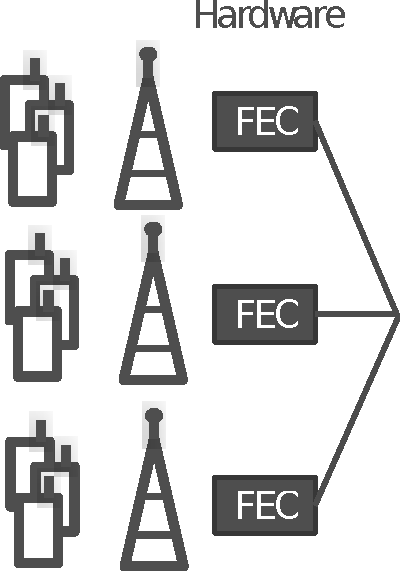
\includegraphics[scale=0.5]{main/ch2_fig/bs}
  \label{fig:bs}
  }
  \quad\quad
  \subfloat[Séparation BB / RF]{
  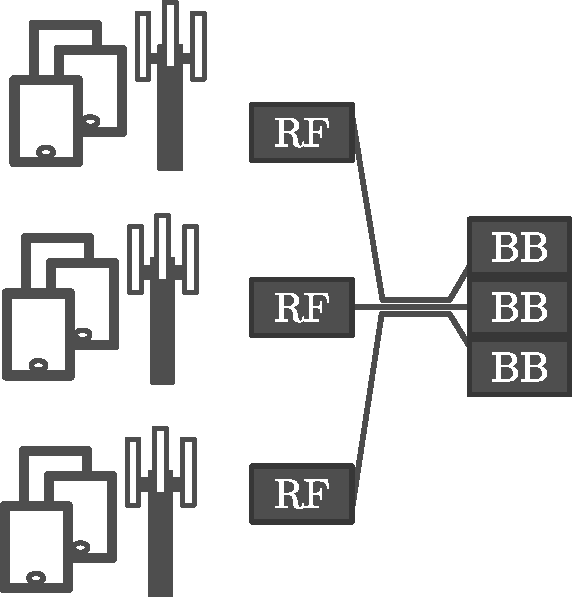
\includegraphics[scale=0.5]{main/ch2_fig/bs2}
  \label{fig:bbu}
  }
  \quad\quad
  \subfloat[Cloud-RAN]{
  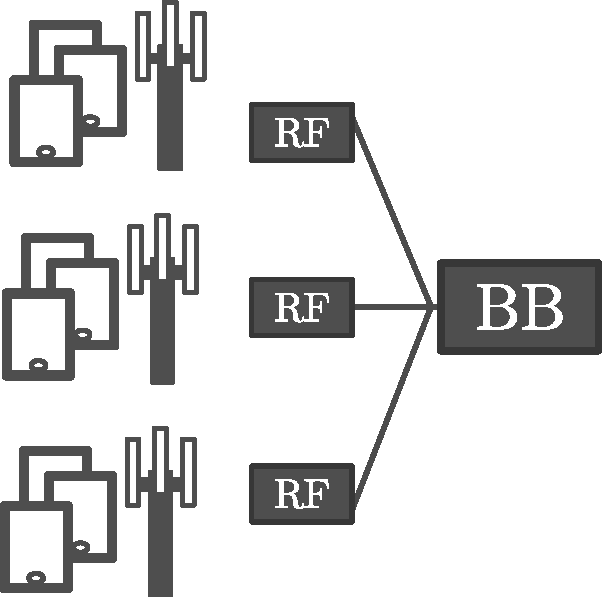
\includegraphics[scale=0.5]{main/ch2_fig/c-ran}
  \label{fig:c-ran}
  }
  \caption{\'Evolution de l'architecture des stations de base}
  \label{fig:bs_evo}
\end{figure}

Ce chapitre est divisé comme suit. Tout d'abord, la section~\ref{sec:art_scl} présente l'état de l'art des implémentations logicielles de l'algorithme SCL sur des processeurs à usage général. Dans cette même section, nous présentons les principales techniques permettant d'atteindre de hauts débits et de faibles latences. 
Nous décrivons ensuite les implémentations proposées qui ont la propriété d'être flexibles et génériques. Dans un souci de clarté, la section~\ref{sec:gen_scl} définit précisément ces concepts de généricité et de flexibilité qui sont au \coeur de l'étude. La section \ref{sec:opti_scl} détaille les optimisations d'implémentation que nous proposons. Ces dernières permettent d'atteindre des débits et des latences compétitifs tout en conservant des caractères génériques et flexibles. Enfin, la section~\ref{sec:exp_scl} compare les différentes implémentations proposées avec des implémentations de l'état de l'art.

\section{\'Etat de l'art sur les implémentations logicielles de l'algorithme SCL}
\label{sec:art_scl}
Les deux principales techniques d'implémentation logicielle permettant d'atteindre de hauts débits et de réduire la latence de décodage des codes polaires sont la vectorisation et le déroulage du code source. Cette section présente ces deux techniques d'implémentation logicielle.

\subsection{Vectorisation}


Les processeurs à usage général (GPPs : General Purpose Processors) actuels sont équipés d'unités de calcul vectoriel SIMD (Single Instruction Mutiple Data). Les architectures de processeurs x86-64 définissent par exemple des jeux d'instructions SIMD nommés SSE (Streaming SIMD Extension) et AVX (Advanced Vector Extensions). Ces jeux d'instructions contiennent des opérations de chargement et de sauvegarde. Ces opérations permettent d'accéder aux données en mémoire et de les déplacer dans le fichier de registres. Ils intègrent également des opérations de calcul, comme les additions, soustractions ou multiplications.
\begin{figure}[htp]
\lstset{language=C++,
        basicstyle=\footnotesize\ttfamily,
        keywordstyle=\bfseries\color{green!40!black},
        commentstyle=\itshape\color{purple!40!black},
        identifierstyle=\color{blue},
        stringstyle=\color{orange},
        morecomment=[l][\color{magenta}]{\#}
}
\begin{lstlisting}[language=C++, numbers=left, numbersep=0.3em, tabsize=2, basicstyle=\footnotesize\ttfamily]
class API_polar
{
  // l'usage de templates permet le support de différents formats
  // de données : virgule fixe, virgule flottante, nombre de bits
  template <typename R>
  // le type "Reg" permet l'accès aux registres vectoriels
  mipp::Reg<R> f_simd(const mipp::Reg<R> &la,
                      const mipp::Reg<R> &lb)
  {
    // toutes les opérations nécessaires aux fonctions polaires
    // sont vectorisées (abs, min, sign, neg)
    auto abs_la  = mipp::abs(la);
    auto abs_lb  = mipp::abs(lb);
    auto abs_min = mipp::min(abs_la, abs_lb);
    auto sign    = mipp::sign(la, lb);
    auto lc      = mipp::neg(abs_min, sign);

    return lc;
  }

  template <typename B, typename R>
  mipp::Reg<R> g_simd(const mipp::Reg<R> &la,
                      const mipp::Reg<R> &lb,
                      const mipp::Reg<B> &sa)
  {
    auto neg_la = mipp::neg(la, sa);
    // MIPP supporte également la surcharge d'opérateurs
    auto lc     = neg_la + lb;

    return lc;
  }

  \end{lstlisting}
  \caption{Implémentation logicielle des fonctions $f$ et $g$ utilisant la bibliothèque MIPP.}
  \label{fig:mipp}
  \end{figure}

Réduire le temps d'exécution des algorithmes de décodage de codes polaires à l'aide d'instructions SIMD est une technique classique utilisée dans de nombreuses implémentations de l'algorithme SC \cite{sarkis_fast_2014,giard_fast_2014,giard_low-latency_2016,sarkis_autogenerating_2014,gal_software_2014,cassagne_efficient_2015,cassagne_energy_2016,gal_multi-gb/s_2015} comme de l'algorithme SCL \cite{sarkis_fast_2016,sarkis_increasing_2014,shen_low-latency_2016}. Nous utilisons dans nos travaux une bibliothèque générique et portable implémentant les fonctions élémentaires des codes polaires \cite{cassagne_efficient_2015}. Elle est basée elle-même sur la bibliothèque MIPP \cite{cassagne2018mipp} qui est une encapsulation des instructions SIMD dont la description logicielle est écrite en langage C++.

L'utilisation de cette bibliothèque présente plusieurs avantages. D'une part le code source apparaît clair, lisible et compact, contrairement à ce qui serait obtenu en utilisant un langage assembleur. Un extrait du code est donné dans la Figure~\ref{fig:mipp}. D'autre part, le code source est portable puisqu'il est compatible avec différentes cibles architecturales (Intel x86, Xeon KNL et ARM) à travers l'utilisation de différents jeux d'instructions (SSE, AVX et NEON). Enfin, MIPP permet d'utiliser plusieurs formats de représentation des données, à savoir : la virgule flottante sur des mots de 32 ou 64 bits et virgule fixe sur des mots de 8, 16, 32 ou 64 bits. Plus le nombre de bits utilisés pour représenter une donnée est faible, plus le parallélisme résultant est important. Ainsi, le jeu d'instruction AVX2 permet de manipuler et de réaliser des opérations sur des registres de 256 bits. Si les données manipulées sont représentées sur 8 bits, alors le niveau de parallélisme est de 64. En clair, 64 opérations peuvent être alors réalisées en parallèle. Il est à noter que la versatilité de la bibliothèque MIPP est obtenue sans perte de performance de décodage comme démontré dans \cite{cassagne2018mipp}.

Comme évoqué dans la sous-section \ref{subsubsec:parallel}, dans le contexte du décodage de codes polaires, il existe deux stratégies principales de parallélisation. Le parallélisme est utilisé soit pour décoder plusieurs trames en parallèle (\textit{inter-trame}), soit pour accélérer le décodage de chaque trame prise individuellement (\textit{intra-trame}). Dans les travaux présentés ici, seule la stratégie \textit{intra-trame} est utilisée. En effet cette dernière permet d'obtenir des latences plus faibles que dans le cas d'une stratégie \textit{inter-trame}. Le principe de la stratégie \textit{intra-trame} est d'appliquer simultanément plusieurs fonctions polaires élémentaires ($f$, $g$ ou $h$) sur un ensemble de données contenues dans un \noeud de l'arbre. Il est également possible d'utiliser des instructions SIMD pour réaliser les opérations sur les données contenues dans les feuilles. En effet, que ce soit dans les feuilles de type \texttt{R1}, \texttt{REP} ou \texttt{SPC}, il est nécessaire d'effectuer des opérations de seuillage sur un nombre de LLR correspondant à la taille du \noeud. Ce seuillage est effectué en parallèle sur tous les LLR du \noeud considéré grâce à des instructions SIMD.

Toutefois, le parallélisme \textit{intra-trame} n'est exploitable que dans la partie supérieure de l'arbre. \`A ce niveau, les \noeuds contiennent un nombre de données supérieur au niveau de parallélisme des unités SIMD. Dans le bas de l'arbre, près des feuilles, la bibliothèque MIPP \cite{cassagne_efficient_2015} utilise automatiquement les versions séquentielles des implémentations des fonctions élémentaires. Dans le cas de l'algorithme CASCL sur un code polaire de taille (2048, 1723), l'augmentation du débit obtenu par l'utilisation des instructions AVX2 sur un processeur Intel i7 6600K est d'environ 20\% pour les décodeurs proposés.

\subsection{Déroulage du code source}
\label{subsec:unroll}
La seconde technique classique que nous retrouvons dans les travaux récents est le déroulage du code source \cite{sarkis_autogenerating_2014,giard_fast_2014,cassagne_efficient_2015,cassagne_energy_2016}. Il découle de l'observation faite sur les décodeurs implémentant l'algorithme SC que les différents tests nécessaires au parcours de l'arbre de décodage prennent un temps significatif. Le parcours de l'arbre étant une donnée statique de l'algorithme de décodage, il est ainsi possible d'éviter ces tests en \og déroulant \fg le code source avant la compilation. La Figure~\ref{fig:unrolling} est une illustration de ce déroulage. D'un côté, dans le code non déroulé de la Figure \ref{fig:alg_rolled}, des appels récursifs potentiellement coûteux de la fonction \textit{DecodeNode} sont réalisés. De plus, des branchements conditionnels sont nécessaires pour traiter des feuilles de types différents (\texttt{R0}, \texttt{R1}, \texttt{REP} ou \texttt{SPC}). Au contraire, dans l'implémentation de la Figure~\ref{fig:alg_unrolled}, ni appel récursif ni branchement conditionnel ne sont nécessaires. Seules les fonctions élémentaires polaires sont appelées.

Il est à noter que l'arbre de décodage que nous prenons en exemple, dans la Figure~\ref{fig:unrolled_tree}, n'est pas élagué. Lors du décodage d'un arbre élagué, le nombre de tests effectués au cours du parcours de l'arbre augmente en proportion du nombre total d'instructions. Cela résulte du fait que le nombre de fonctions polaires différentes augmente. En effet, les fonctions \texttt{REP} et \texttt{SPC} sont ajoutées ainsi que des versions différentes des fonctions $f$, $g$ et $h$ prenant en compte l'existence de \noeuds spécialisés dans l'arbre élagué, comme décrit dans \cite{sarkis_fast_2014,cassagne_efficient_2015}. Dans certains cas, le déroulage du code source permet d'augmenter jusqu'à un facteur 2 les débits de décodage \cite{sarkis_autogenerating_2014}. Cette technique de déroulage a été également étendue pour l'algorithme de décodage SCL \cite{sarkis_fast_2016}.

  \begin{figure}[t]
  \subfloat[Code non déroulé.]{
  \begin{minipage}{.35\linewidth}
  	\LinesNumberedHidden
    \begin{algorithm}[H]
      \SetAlgoLined
      \textit{DecodeNode}($\mathcal{N}_{0,0}$)\;
	  \SetKwProg{Fn}{Function}{}{}
	  \Fn{DecodeNode ($\mathcal{N}_{i,j}$)}{
	    \eIf{i<n}
	    {
	     $f(\mathcal{N}_{i,j})$\;
	     \textit{DecodeNode}($\mathcal{N}_{i+1,2j}$) \;
	     $g(\mathcal{N}_{i,j})$\;
	     \textit{DecodeNode}($\mathcal{N}_{i+1,2j+1}$) \;
	     $h(\mathcal{N}_{i,j})$\;
	    }
	    {
	      \eIf{$\mathcal{N}_{i,j}$\text est gelé}
	      {\texttt{R0}($\mathcal{N}_{i,j}$)\;}
	      {\texttt{R1}($\mathcal{N}_{i,j}$)\;}
	    }
      }
      \caption{Non Déroulé}%
    \end{algorithm}%
  \end{minipage}%
  \label{fig:alg_rolled}
  } 
  \quad\quad
  \subfloat[Code déroulé.]{
  \begin{minipage}{.16\linewidth}
    \LinesNumberedHidden
    \begin{algorithm}[H]
    \setstretch{1.045}
      \SetAlgoLined
	  $f(\mathcal{N}_{0,0})$\;
	  $f(\mathcal{N}_{1,0})$\;
	  \texttt{R0}($\mathcal{N}_{2,0}$)\;
	  $g(\mathcal{N}_{2,1})$\;
	  \texttt{R0}($\mathcal{N}_{2,1}$)\;
	  $h(\mathcal{N}_{1,0})$\;
	  $g(\mathcal{N}_{0,0})$\;
	  $f(\mathcal{N}_{1,1})$\;
	  \texttt{R1}($\mathcal{N}_{2,2}$)\;
	  $g(\mathcal{N}_{1,1})$\;
	  \texttt{R1}($\mathcal{N}_{2,3}$)\;
	  $h(\mathcal{N}_{1,1})$\;
	  $h(\mathcal{N}_{0,0})$\;
	  \mbox{}\\
      \caption{Déroulé}%
    \end{algorithm}%
  \end{minipage}%
  \label{fig:alg_unrolled}
  }
  \subfloat[Arbre décodé.]{
  \begin{minipage}{.35\linewidth}
  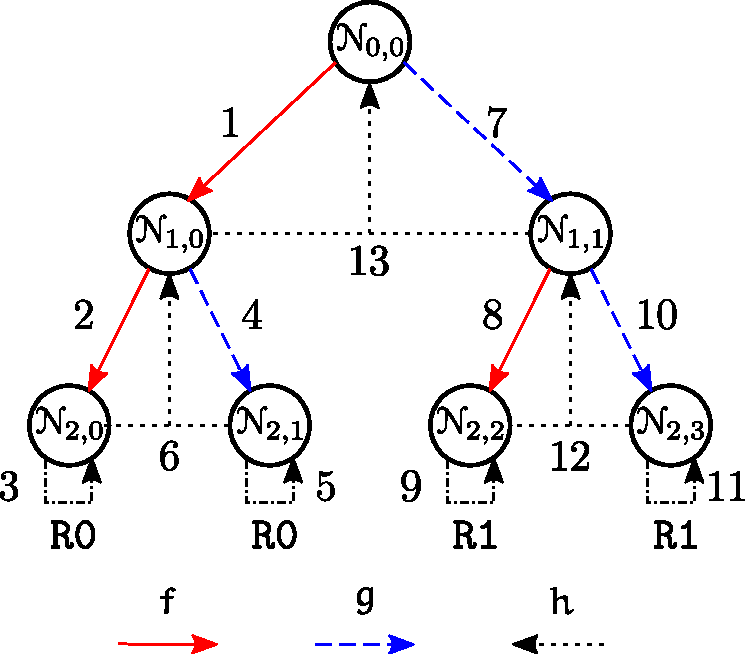
\includegraphics[width=\linewidth]{main/ch2_fig/unrolled_tree}
  \label{fig:unrolled_tree}
  \end{minipage}%
  }
  \caption{Déroulage du code source décrivant l'algorithme de décodage SC non élagué d'un code polaire (4,2) systématique.}
  \label{fig:unrolling}
\end{figure}

Les résultats d'implémentation logicielle au niveau des débits et latences des différents décodeurs reportés dans la littérature \cite{sarkis_increasing_2014,sarkis_fast_2016,shen_low-latency_2016} sont récapitulés et discutés dans la section \ref{sec:exp_scl}, dans le tableau \ref{tab:res} accompagnés des résultats des décodeurs proposés.

\section{Généricité et flexibilité d'un décodeur de codes polaires}
\label{sec:gen_scl}

\subsection{Définitions}
Les termes de généricité et de flexibilité pouvant donner lieu à diverses interprétations, nous proposons d'en donner une définition pour éviter toute ambiguïté.
Nous parlerons de la \textit{généricité} comme étant la capacité d'un décodeur à supporter n'importe quel encodage.
En effet, dans le contexte de communications mobiles, les paramètres de l'encodeur changent constamment pour s'adapter au canal. Pour ce faire, des méthodes adaptatives de modulation et de codage \cite{dahlman_4g:_2013} (AMC : Adaptive Modulation and Coding) sont appliquées. Ainsi, la taille du code polaire, le rendement de codage ou bien encore la position des bits gelés peuvent varier d'une trame à une autre. Par ailleurs, des patrons de poinçonnage sont souvent nécessaires. Enfin, des codes CRC sont concaténés aux codes polaires afin de détecter les erreurs et permettre des méthodes de transmission à demande de répétition automatique (ARQ : Automatic Repeat reQuest) ou leur évolution hybride (HARQ : Hybrid ARQ). Un décodeur générique devrait donc supporter toutes les combinaisons possibles de chacun de ces paramètres.

D'autre part, le terme \textit{flexibilité} s'appliquera au paramétrage de l'algorithme et des méthodes d'implémentation du décodeur, indépendamment du schéma de codage. Ces paramètres ne sont généralement pas imposés par la norme de communication. Dans le cas de l'algorithme SCL, les paramètres suivants sont concernés : les variantes de l'algorithme (FASCL, PASCL), le format de représentation des données (virgule flottante ou fixe, nombre de bits), la taille de la liste $L$ ou encore l'élagage de l'arbre de décodage. La flexibilité du décodeur amène des degrés de liberté à l'implémentation permettant des compromis entre performances de décodage, latence et débit, pour un schéma d'encodage donné.

Comme nous allons le détailler dans les sections suivantes, tous les paramètres de généricité et de flexibilité cités sont supportés dans les implémentations de décodeurs proposées. Ils sont déterminés de manière dynamique à l'aide de fichiers de configuration ou des arguments de ligne de commande, lus lors de l'exécution. Aucune compilation du code source n'est nécessaire en cas de changement d'un paramètre. De ce choix découle le fait que nous n'utilisons pas la technique de déroulage présentée dans sous-section \ref{subsec:unroll}. En effet, cette technique implique la génération d'un code source pour chaque combinaison de paramètres comme proposé dans \cite{sarkis_autogenerating_2014} pour l'algorithme SC.

\subsection{Généricité}

\begin{figure}[t]
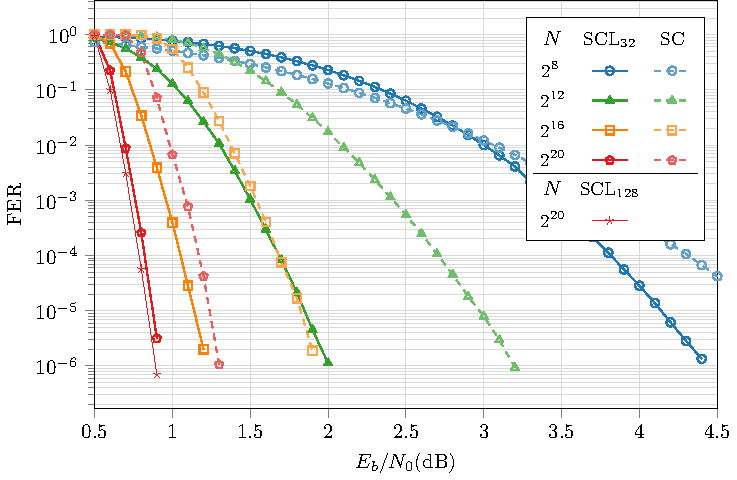
\includegraphics[width=\textwidth]{main/ch2_fig/curves/code/tikz/code}
\caption{Performances de décodage des algorithmes SC et CASCL pour des très grandes tailles de code, $R=1/2$, CRC $c=32$ (GZip)}
\label{fig:large_scl}
\end{figure}

Les implémentations logicielles de décodeur proposées s'appliquent à n'importe quelle taille de mot de code. De plus, les débits des décodeurs étant compétitifs, il est possible d'explorer de grandes tailles de code conjointement à des profondeurs de liste importantes, comme montré dans la Figure~\ref{fig:large_scl}. Dans ce cas, $N$ prend des valeurs allant de $2^8$ à $2^{20}$ et le rendement du code polaire est $R=1/2$. Le CRC utilisé est défini dans le norme GZip : sa longueur est $c=32$ et son polynôme \texttt{0x04C11DB7}. 
Des simulations de performances de décodage de l'algorithme CASCL pour des codes polaires de grande taille ($N \geq 2^{14}$) sont rares dans la littérature. La seule référence disponible présente les performances de décodage de l'algorithme CASCL pour un code polaire ($32768$,$29504$) avec $L=4$.
L'algorithme SCL a été proposé pour améliorer les performances de décodage des codes polaires pour de petites tailles ($N<2^{12}$). Néanmoins, le fort débit du décodeur logiciel proposé permet de montrer que son utilisation pour des codes polaires de grande taille apporte également un gain significatif au niveau des performances de décodage. Dans le cas où $N=2^{12}$, l'utilisation de l'algorithme CASCL avec une taille de liste $L=32$ apporte un gain d'environ 1.2 dB lorsque le FER est égal à $10^{-5}$. Cependant, ce gain diminue lorsque $N$ augmente : 0.75 dB pour $N=2^{16}$ et 0.5 dB pour $N=2^{20}$. Des simulations ont également été réalisées pour une profondeur de liste $L=128$. Elles montrent que le gain par rapport à $L=32$ n'est pas significatif.

\subsection{Flexibilité}
Les paramètres de flexibilité sont eux aussi configurables lors de l'exécution du programme. Ils permettent divers compromis entre la latence, le débit et les performances de correction. Ainsi, l'algorithme de décodage peut être ajusté pour un code polaire donné. Dans la suite de cette section, ces paramètres de flexibilité sont détaillés et leurs effets analysés.

\subsubsection{Profondeur de la liste}
\begin{figure}[t]
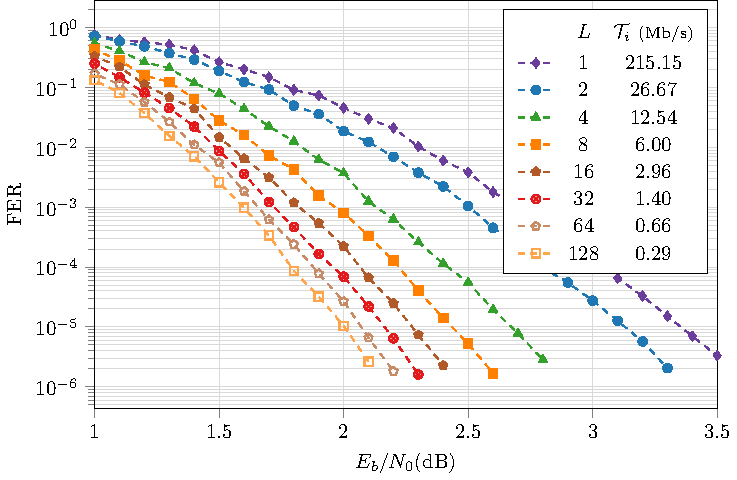
\includegraphics[width=\textwidth]{main/ch2_fig/curves/L/tikz/L}
\caption{Performances de décodage et débits de l'algorithme CASCL pour différentes valeurs de $L$ d'un code polaire ($2048,1024$) concaténé à un CRC $c=32$ (GZip).}
\label{fig:scl_l_thr}
\end{figure}
La profondeur de la liste impacte directement le pouvoir de correction et la complexité calculatoire de l'algorithme. La Figure~\ref{fig:scl_l_thr} représente les performances au niveau FER et les débits obtenus pour l'algorithme de décodage CASCL d'un code polaire ($2048$,$1024$). La complexité calculatoire augmente linéairement. Le débit est divisé approximativement par deux lorsque la profondeur de liste $L$ est doublée. Le seul cas ne respectant pas cette tendance est celui pour lequel $L=1$ qui correspond à l'algorithme SC. Ce dernier est bien plus rapide puisqu'il ne nécessite pas d'effectuer les calculs associés à l'algorithme SCL comme le tri, la génération des candidats, le calcul du CRC. Le FER évolue également avec $L$. \`A partir de $L\geq4$ et $E_b/N_0=2dB$, les performances au niveau FER diminuent continûment, de $4.10^{-3}$ à $10^{-5}$.

\subsubsection{Paramétrage fin de l'élagage}
L'élagage tel que défini dans la sous-section~\ref{subsec:pruning} est paramétrable très finement dans les implémentations de décodeurs polaires proposées. Tout d'abord, chaque type de \noeud (\texttt{R0}, \texttt{R1}, \texttt{REP} et \texttt{SPC}) peut être activé ou désactivé séparément. Cette caractéristique est utile pour analyser l'impact de l'utilisation de chaque type de \noeud sur le débit de décodage.

\`A ce stade, il est important de faire la distinction entre le débit codé et le débit d'information. Soit $\mathcal{T}_F$, le nombre de mots de code décodés par seconde. Dans ce cas, la valeur du débit d'information est $\mathcal{T}_i=K\mathcal{T}_F$, soit le nombre de bits d'informations décodés par seconde, tandis que la valeur du débit codé est $\mathcal{T}_c=N\mathcal{T}_F$.

Pour explorer l'impact de l'utilisation des types de \noeuds sur le débit, il apparaît plus pertinent d'utiliser le débit codé. En effet, si le débit d'information était utilisé dans la Figure~\ref{fig:nodes}, le rendement du code \og biaiserait \fg les débits. En effet, les débits des codes à haut rendement seraient supérieurs à ceux des codes à faible rendement.
\begin{figure}[t]
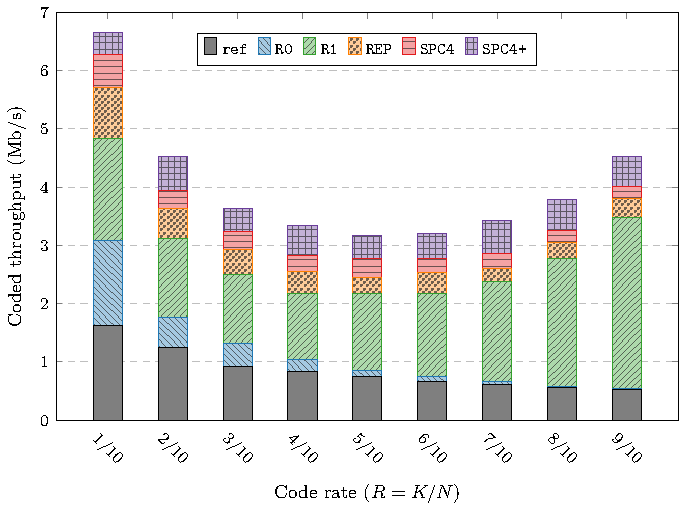
\includegraphics[width=\textwidth]{main/ch2_fig/curves/tree/tikz/tree}
\caption{Impact de l'activation des \noeuds d'élagage de l'algorithme CASCL, $N=2048$, $L=32$, $c=32$.}
\label{fig:nodes}
\end{figure}

\begin{figure}[t]
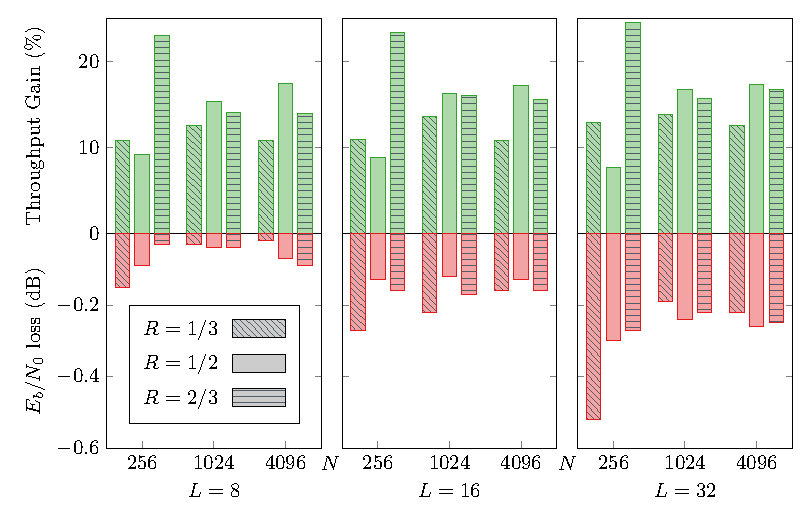
\includegraphics[width=\textwidth]{main/ch2_fig/curves/thr_spc/tikz/thr_spc_diff}
\caption{Effets de l'utilisation des \noeuds \texttt{SPC4+} dans l'algorithme CASCL pour un FER de $10^{-5}$}
\label{fig:spc_impact}
\end{figure}

Le débit codé de l'algorithme non élagué (\texttt{ref}) diminue lorsque le rendement augmente. Cela s'explique par le fait que les feuilles de rendement 1, plus nombreuses dans des codes à haut rendement, nécessitent plus de temps pour être décodées que les feuilles de rendement 0. En effet, dans l'algorithme SCL, le traitement d'une feuille de rendement 0 correspond à la mise à jour de métriques. Par ailleurs, le traitement d'une feuille de rendement 1 correspond à la génération de candidats, à la mise à jour de leurs métriques, au tri de celles-ci et à des duplications d'arbres de décodage.

Dans la Figure \ref{fig:nodes}, les aires hachurées en diagonales (\raisebox{-\mydepth}{
\includegraphics[height=\myheight]{main/ch2_fig/hach1}},\raisebox{-\mydepth}{
\includegraphics[height=\myheight]{main/ch2_fig/hach2}}) représentent l'amélioration des performances de décodage lorsque les \noeuds \texttt{R0} et \texttt{R1} de tailles supérieures à un sont utilisés pour l'élagage. De manière attendue, l'élagage \texttt{R1} favorise une augmentation plus significative du débit pour les codes à haut rendement. Inversement, l'élagage \texttt{R0} s'avère plus efficace pour des codes à faible rendement. Une même tendance est observée pour l'élagage des \noeuds \texttt{REP}. Ces derniers sont plus efficaces pour des codes de faibles rendements. En effet, les \noeuds \texttt{REP} sont plus abondants dans les codes à faibles rendements. En revanche, la tendance est moins claire pour les \noeuds \texttt{SPC}.

Il est observé dans \cite{sarkis_fast_2014} que lorsque la taille des \noeuds \texttt{SPC} n'est pas limitée à 4, les performances de décodage peuvent être dégradées. Dans les implémentations logicielles proposées, le choix a été fait de donner la possibilité de paramétrer finement la taille des \noeuds activés pour chaque type de \noeuds. En conséquence, leur taille est limitée à 4 dans les aires étiquetées \texttt{SPC4} dans la Figure \ref{fig:nodes}. Les aires étiquetées \noeuds \texttt{SPC4+} correspondent aux débits atteints lorsque la taille des \noeuds \texttt{SPC} n'est plus limitée à 4.

Dans nos expérimentations, la dégradation au niveau des performances de décodage due à l'utilisation des \noeuds \texttt{SPC4+} n'est pas systématique mais dépendante des caractéristiques du code polaire considéré. La Figure~\ref{fig:spc_impact} illustre le compromis entre le débit du décodeur et les performances de décodage lorsque les \noeuds \texttt{SPC4+} sont utilisés. La partie supérieure représente le débit du décodeur et la partie inférieure indique la dégradation induite pour les différents codes polaires considérés. Les augmentations de débits sont comprises entre 8\% et 20\% selon les cas, c'est-à-dire selon la profondeur de la liste, de la taille du mot de code et du rendement. La partie inférieure de la Figure \ref{fig:spc_impact} illustre pour sa part la dégradation des performances de décodage. Pour une profondeur de liste $L=8$, en dehors d'une configuration particulière ($N=256$, $R=1/3$), la dégradation du SNR pour un FER de $10^{-5}$ est inférieure à 0.1 dB. Si $L=32$ alors la dégradation est généralement légèrement supérieure à 0.2 dB. Encore une fois, le cas du code polaire ($N=256$, $R=1/3$) est problématique avec une dégradation d'environ 0.5 dB.

En conclusion, l'élagage de l'arbre permet des augmentations significatives du débit des décodeurs logiciels de l'algorithme SCL. Toutefois le traitement des \noeuds \texttt{SPC4+} décrit dans \cite{sarkis_fast_2016} peut provoquer une dégradation des performances de décodage qui dépend des paramètres de l'algorithme. Des tests complémentaires seraient nécessaires pour quantifier exhaustivement leur impact. La forte généricité et la grande flexibilité du décodeur logiciel proposé facilitent l'exploration de ce compromis entre performance de décodage et débit. Il est important de noter que l'activation des \noeuds d'élagage est effectuée dynamiquement. Aussi, il serait possible de développer un décodeur logiciel qui adapterait dynamiquement son élagage, en temps réel, en fonctions des contraintes systèmes.

\subsubsection{Représentation en virgule fixe}

Il existe deux formats de représentation des nombres en base 2 : la représentation en virgule flottante et la représentation en virgule fixe. La représentation en virgule flottante offre une plus grande dynamique. Quant à la représentation en virgule fixe, elle simplifie les opérations arithmétiques. L'avantage des décodeurs de canal est que les données manipulées sont des données de type probabiliste. \`A ce titre, ces algorithmes sont souvent robustes vis-à-vis d'une diminution du nombre de bits utilisés pour représenter les données et par conséquent d'une représentation en virgule fixe.
L'avantage de représenter les données à l'aide d'un nombre réduit de bits est que cela permet aux unités SIMD d'effectuer davantage d'opérations en parallèle. 
L'objectif est donc de réduire le nombre de bits afin d'augmenter le parallélisme et par conséquence les performances de débit et de latence.

Des implémentations logicielles quantifiées de l'algorithme SC ont déjà été proposées \cite{giard_low-latency_2016} dans la littérature.
 Cependant, les décodeurs proposés constituent, à la connaissance de l'auteur, la première implémentation logicielle de l'algorithme SCL permettant de représenter les LLR et les métriques de chemin sur 8 ou 16 bits.
Pour que la représentation en virgule fixe n'introduise pas de dégradation, des précautions doivent être prises.
Tout d'abord, pour des représentations sur 8 bits, les LLR et les métriques de chemin sont saturés entre -127 et +127 après chaque opération.
De plus, les métriques de chemin sont normalisées après chaque opération de duplication et de sélection de candidats. Cela signifie que la valeur la plus faible des métriques de chemin est soustraite à chacune d'entre elles.
La Figure~\ref{fig:bfer_rep} montre les performances de l'algorithme CASCL pour différentes représentations des LLR : 8 bits à virgule fixe, 16 bits à virgule fixe et 32 bits à virgule flottante.
Les courbes pour 32 bits et 16 bits sont confondues et montrent que la représentation sur 16 bits ne dégrade pas les performances. En revanche, des dégradations apparaissent pour la courbe pour 8 bits, étiquetée \texttt{REP2+}.
Après analyse, il s'avère que ces dégradations sont dues au décodage des \noeuds de répétition.
En effet, lors de ce traitement, comme détaillé en sous-section \ref{subsec:pruning}, il faut sommer tous les LLR du \noeud considéré.
Or pour un \noeud de répétition de grande taille, cette addition sur 8 bits peut induire un débordement.
La Figure \ref{fig:bfer_rep} montre que lorsque les \noeuds de répétition de taille supérieure à 8 sont désactivés (\texttt{REP8-}), ces débordements n'ont plus lieu et les performances sont similaires à celles d'un décodage effectué au format 32 bits à virgule flottante.

\begin{figure}
\centering
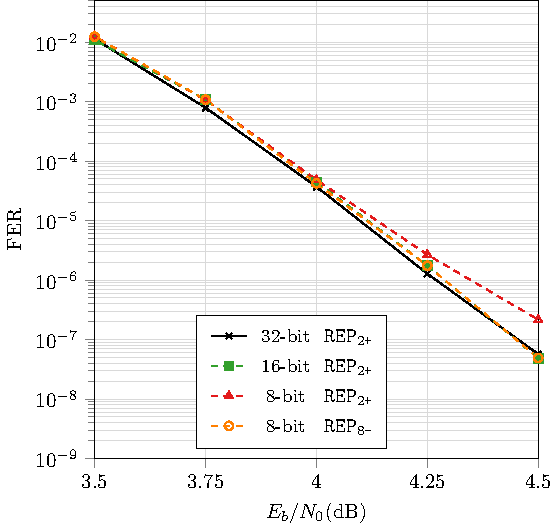
\includegraphics{main/ch2_fig/curves/bfer/tikz/bfer_rep}
\caption{Impact de l'utilisation des \noeuds de répétition sur des implémentations quantifiées.}
\label{fig:bfer_rep}
\end{figure}
  \begin{table}[b]
    \renewcommand{\arraystretch}{1.1}
    \centering
    \caption{Comparaison de débits et latences des algorithmes SCL adaptatifs pour des représentations à virgule flottante (32 bits) et virgule fixe (16 et 8 bits). Code polaire ($2048$,$1723$), $L=32$, CRC $c=32$ (GZip)}
    \label{tab:quantif}
    {\small\resizebox{\linewidth}{!}{
    \begin{tabular}{r | c | c || c | c || c | c || c | c}
      \multirow{2}{*}{\textbf{Décodeur}} & \multirow{2}{*}{\textbf{Quantif.}} & \multirow{2}{*}{$\bm{\mathcal{L}_{PC}}$} & \multicolumn{2}{c ||}{\textbf{3.5 dB}} & \multicolumn{2}{c ||}{\textbf{4.0 dB}} & \multicolumn{2}{c}{\textbf{4.5 dB}} \\
      \cline{4-9}
      & & & $\bm{\mathcal{L}_{moy}}$ & $\bm{\mathcal{T}_i}$ & $\bm{\mathcal{L}_{moy}}$ & $\bm{\mathcal{T}_i}$ & $\bm{\mathcal{L}_{moy}}$ & $\bm{\mathcal{T}_i}$ \\
      % \hline
      \hline
      \multirow{3}{*}{PA-SSCL} & 32-bit &  635 & 232.3 &   7.6 & 41.7 &  42.1 & 7.4 & 237.6 \\
      %\cline{3-9}
                               & 16-bit &  622 & 219.6 &   8.0 & 40.1 &  43.8 & 6.6 & 267.5 \\
      %\cline{3-9}
                               &  8-bit &  651 & 232.4 &   7.6 & 41.2 &  42.6 & 6.5 & 268.3 \\
      \hline
      \multirow{3}{*}{FA-SSCL} & 32-bit & 1201 &  67.2 &  26.1 &  8.5 & 207.8 & 5.1 & 345.5 \\
      %\cline{3-9}
                               & 16-bit & 1198 &  68.7 &  25.6 &  7.7 & 225.7 & 4.3 & 408.7 \\
      %\cline{3-9}
                               &  8-bit & 1259 &  71.8 &  24.4 &  7.7 & 227.3 & 4.1 & 425.9 \\
    \end{tabular}
    }}
  \end{table}

Dans le tableau \ref{tab:quantif} sont listés la latence \og pire cas \fg ($\mathcal{L}_{PC}$), la latence moyenne ($\mathcal{L}_{moy}$) et le débit d'information moyen ($\mathcal{T}_i$, en Mb/s) des algorithmes adaptatifs, PASCL et FASCL, pour les différentes représentations de l'information. Le processeur sur lequel les tests ont été réalisés est un processeur Intel i7 6600K. Dans le cas de la représentation sur 8 bits, les \noeuds répétitions de taille supérieure à 8 sont désactivés afin d'effectuer les mesures de vitesse pour performances de décodage identiques. Les représentations à virgule fixe réduisent dans la majorité des cas la latence moyenne, surtout dans les régions à fort SNR. Ceci est dû au fait que l'accélération apportée par la représentation en virgule fixe sur une nombre réduit de bits est plus importante pour l'algorithme SC que pour l'algorithme SCL. Or, dans le cas des algorithmes adaptatifs, plus le SNR est élevé, plus il est probable que le décodage SC suffise et qu'il n'y ait pas besoin de réaliser les décodages SCL. Ainsi, un débit de 425.9 Mb/s est atteint pour une représentation sur 8 bits des LLR dans le cas de l'algorithme FASCL. Cela correspond à une augmentation de 80 Mb/s en comparaison avec la représentation sur 32 bits. Les décodeurs décrits montrent donc qu'il est possible d'implémenter les différents algorithmes à liste en représentant les données sur 8 bits sans dégrader les performances. Cette exploitation de la représentation en virgule fixe permet d'accélérer significativement le décodage des  implémentations logicielles des algorithmes à liste.

\begin{figure}[t]
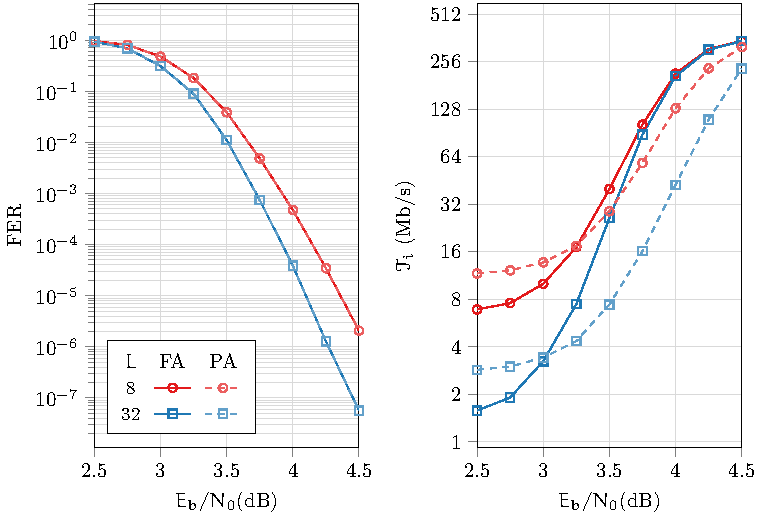
\includegraphics{main/ch2_fig/curves/ascl/tikz/ascl}
\caption{Performances de décodage et débits des algorithmes de décodage PASCL et FASCL pour un code polaire ($2048$,$1723$), $L=32$, et CRC $c=32$ GZip.}
\label{fig:ascl_perfs}
\end{figure}


\subsubsection{Les différentes variantes algorithmiques implémentées}
La Figure~\ref{fig:ascl_perfs} montre les deux versions adaptatives de l'algorithme SCL, à savoir les algorithmes partiellement et complètement adaptatifs (PASCL et FASCL). Des débits différents sont observés suivant le rapport signal à bruit $E_b/N_0$ considéré. Pour de faibles valeurs de SNR, l'algorithme PASCL est plus avantageux. En revanche, l'algorithme FASCL prend l'avantage pour des valeurs intermédiaires, avant que les débits de chaque version se rapprochent pour les valeurs de $E_b/N_0$ les plus élevées.
L'explication de cette observation est la suivante : à faible SNR, la probabilité d'échec de décodage est très forte. La plupart du temps, l'algorithme adaptatif doit déclencher un décodage avec $L=L_{max}$ (ici $L_{max}=32$). Pour l'algorithme PASCL, dans ce cas précis où le décodage avec $L=32$ est nécessaire, deux décodages successifs seront déclenchés : le décodage SC puis le décodage SCL avec $L=32$. Pour l'algorithme FASCL, des exécutions intermédiaires de l'algorithme seront effectuées, pour $L=\{2,4,8,16\}$. En résumé, dans le cas le plus fréquent à faible SNR, l'algorithme PASCL est plus rapide que l'algorithme FASCL.
\`A fort SNR, le cas le plus probable est une réussite du décodage. Lorsque l'algorithme SC est suffisant pour décoder la trame, les algorithmes FASCL et PASCL auront des performances similaires. C'est pourquoi les débits des implémentations des deux algorithmes sont proches pour les valeurs les plus fortes de $E_b/N_0$. Pour des valeurs intermédiaires de SNR, le FASCL présente des débits supérieurs à ceux de l'algorithme PASCL. En effet, l'exécution de l'algorithme SCL avec des valeurs intermédiaires de $L$ est alors pertinent. Cependant, dans tous les cas et comme décrit dans la sous-section \ref{subsubsec:adaptive}, la latence \og pire cas \fg, autrement dit le temps maximum nécessaire pour le décodage d'une trame, est plus élevée pour l'algorithme FASCL. Ce fait est vérifié par la mesure comme reporté dans le Tableau~\ref{tab:quantif}.

La section \ref{sec:gen_scl} a permis de définir les concepts de généricité et de flexibilité du décodeur. Des contributions propres aux décodeurs proposés et liées à leur flexibilité ont également été introduites :

\begin{itemize}
  \item la représentation sur 8 et 16 bits en virgule fixe des données pour les algorithmes à liste,
  \item la configuration dynamique de l'élagage de l'arbre de décodage,
  \item le support de l'algorithme FASCL.
\end{itemize}

Cependant, ces implémentations doivent être compétitives par comparaison avec les décodeurs de la littérature du point de vue du débit et de la latence. Pour ce faire, des améliorations permettant d'atteindre de hauts débits et de faibles latences sont présentées dans la section suivante.

\section{Optimisations de l'implémentation logicielle des décodeurs à liste}
\label{sec:opti_scl}
Cette section \ref{sec:opti_scl} présente trois contributions originales. La première porte sur l'utilisation nouvelle d'un algorithme de tri des métriques et des LLR. La seconde concerne l'accélération du contrôle de redondance cyclique. Enfin, la gestion des sommes partielles est l'objet d'une contribution propre.

\subsection{Algorithme de tri}
Des algorithmes de tri partiel sont appliqués durant plusieurs étapes lors de l'exécution de l'algorithme SCL. Ainsi, les $L$ métriques de chemin les plus faibles doivent être identifiées pour sélectionner les candidats lors des étapes de duplication (étapes (i+1) et (i+3) de la Figure~\ref{fig:scl}). De plus, les 2 LLR ayant les valeurs absolues les plus faibles doivent être identifiés lors du traitement des \noeuds \texttt{R1}. Enfin, les 4 LLR les plus faibles doivent être retenus lors du traitement d'un \noeud \texttt{SPC}. 


Dans \cite{sarkis_fast_2016}, la méthode de tri des LLR dans les \noeuds \texttt{REP} et \texttt{SPC} n'est pas précisée.
Schreier \cite{schreier_tournament_1932} donne une méthode pour identifier les deux plus petits (ou les deux plus grands) éléments d'un ensemble. Cette technique est également détaillée dans \cite{knuth_art_1973}. 
Il a été prouvé que cette méthode est la méthode optimale en termes de nombres de comparaisons deux-à-deux à effectuer.
Ce nombre est égal à $N+\log_2(N)-2$

\begin{figure}[t]
\centering
\subfloat[Identification du plus petit élément.]{
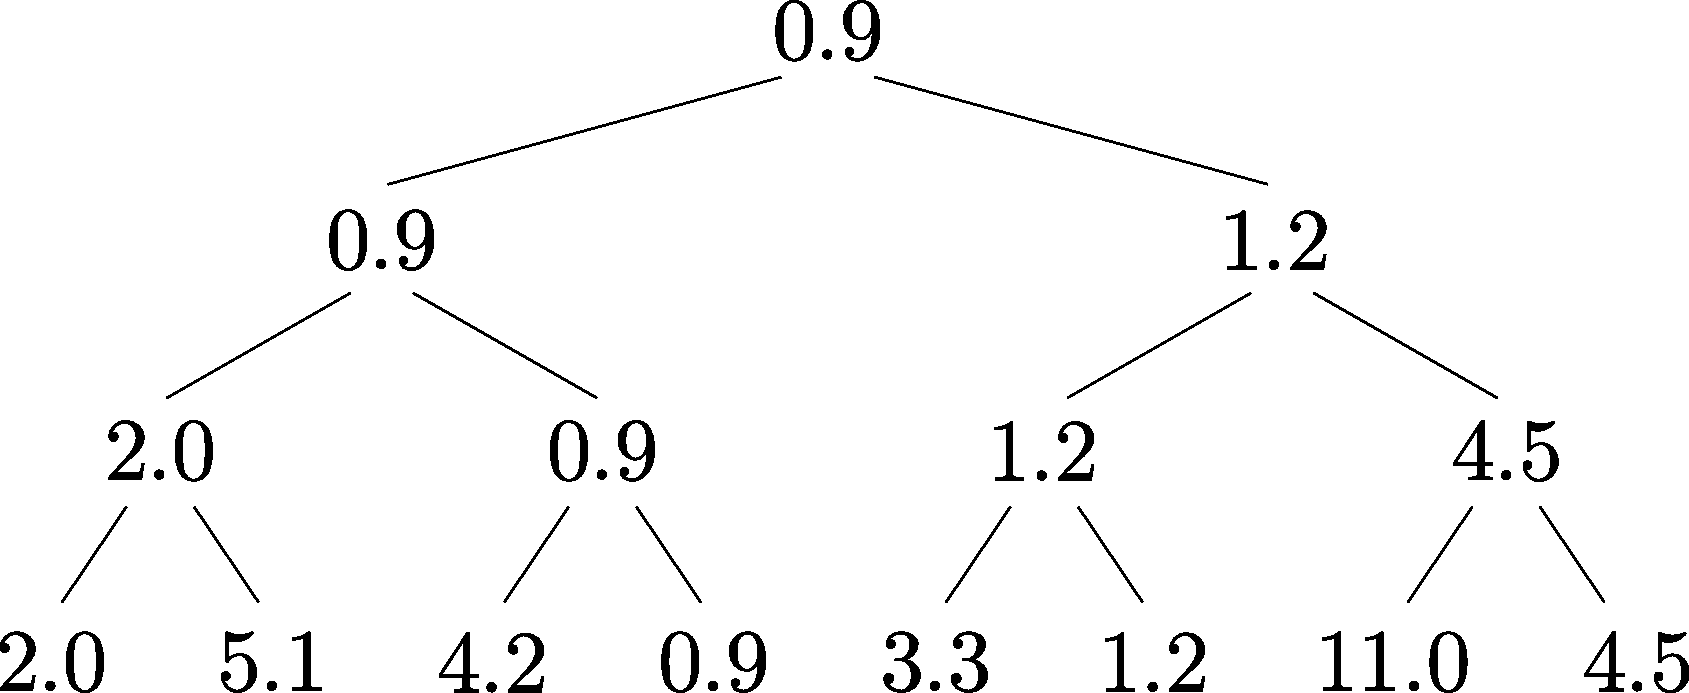
\includegraphics[width=0.75\textwidth]{main/ch2_fig/sorting_a}
\label{fig:sorting_a}
}
\\
\subfloat[Identification du second plus petit élément.]{
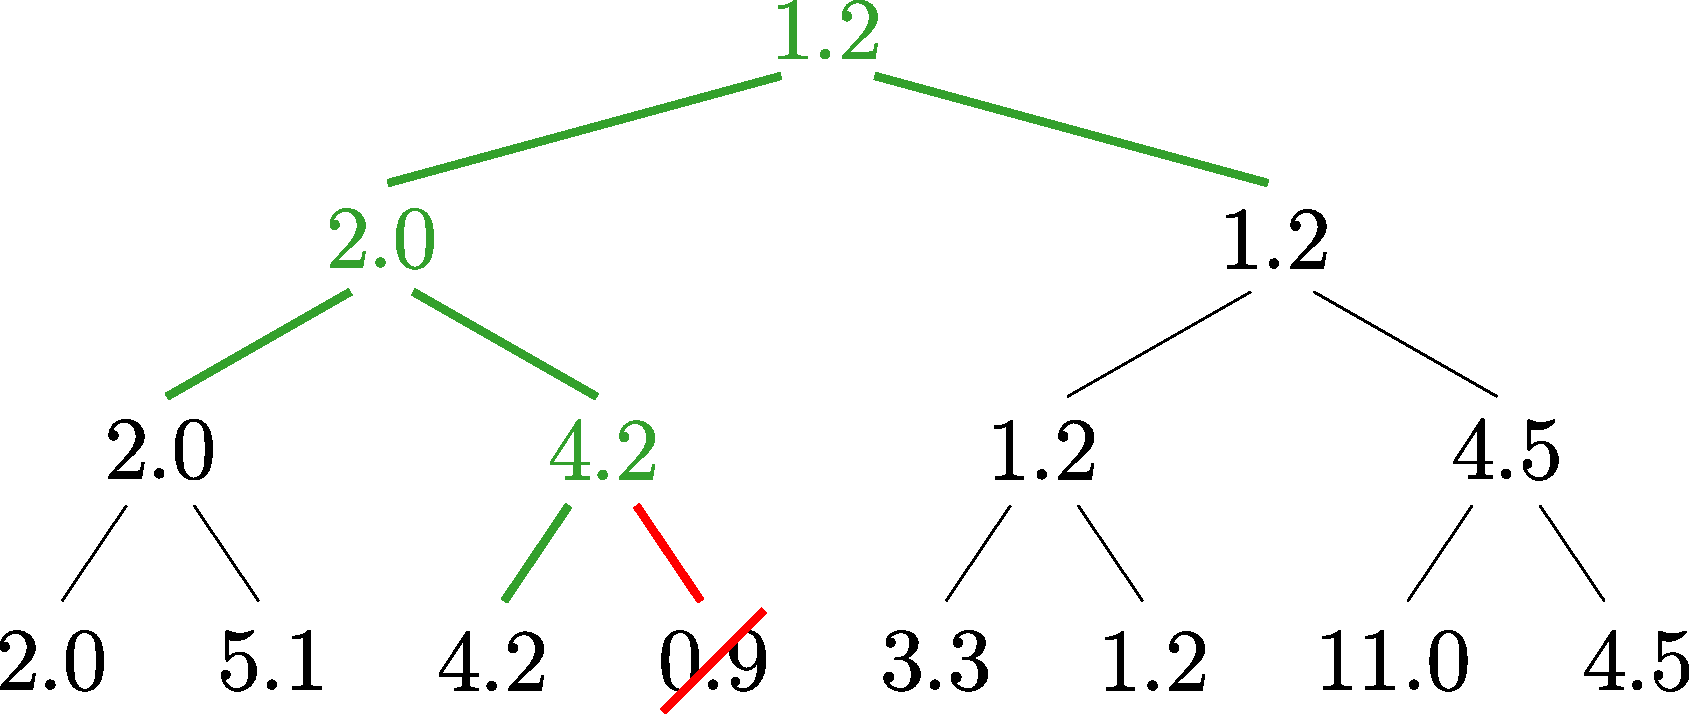
\includegraphics[width=0.75\textwidth]{main/ch2_fig/sorting_b}
\label{fig:sorting_b}
}
\caption{Méthode de Schreier}
\label{fig:schreier_sort}
\end{figure}
Elle nécessite deux étapes complémentaires, présentées en Figure~\ref{fig:schreier_sort}. La première étape est l'identification du plus petit élément par la traversée d'un arbre binaire. Durant la seconde étape, cet élément est éliminé, et la branche sur laquelle il se trouvait est rejouée. Le second élément le plus petit est ainsi identifié.


Cette méthode a été testée expérimentalement et ses performances ont été comparées à d'autres algorithmes potentiels : \textit{Batcher's merge exchange}, tri par bulle, tri \textit{quick-sort}, tri par tas implémenté dans la bibliothèque standard. Les mesures ont été réalisées sur un processeur Intel i7 4790HQ, pour différents rendements, tailles de codes et profondeur de liste. La méthode de Schreier s'est révélée dans tous les cas le plus rapide. Elle l'était également dans les cas testés pour les \noeuds de type \texttt{SPC}. En effet, l'utilisation d'autres algorithmes de tri n'apporte pas de gain significatif.

Le tri des métriques dans \cite{sarkis_fast_2016} est effectué à l'aide d'un réseau de tri partiels (PSN : Partial Sorting Network) décrit dans \cite{furtak2007using}. Les unités de calcul SIMD sont utilisées pour accélérer l'exécution de ce tri. 
Dans un souci de simplicité de la description logicielle, le choix a donc été fait de n'utiliser que la méthode de Schreier pour réaliser les différents tris nécessaires pour l'exécution de l'algorithme SCL.
Dans cette étude, nous n'avons pas implémenté les PSN pour le tri des métriques. En effet, pour que ce réseau de tri soit générique vis à vis de $L$ ainsi que de l'élagage de l'arbre, une méthode devrait être conçue afin de créer un PSN pour n'importe quelle profondeur de liste $L$, et pour chaque type de \noeud différent. Nous pensons que l'utilisation de PSNs pourrait augmenter le débit de nos décodeurs. Toutefois, ce travail n'a pas encore été réalisé, et nous le réservons pour de futurs travaux.
Par défaut, la méthode de Schreier est également utilisée pour le tri des métriques. Les mêmes algorithmes alternatifs ont été testés mais aucune amélioration significative n'a permis d'amélioration du débit.

\subsection{Accélération du contrôle de redondance cyclique}

Par profilage de l'exécution d'un décodeur SCL adaptatif, il est possible d'observer que beaucoup de cycles d'exécution sont alloués aux vérifications de CRC.
En effet, durant chaque décodage (y compris le premier décodage SC), il est nécessaire de réaliser une vérification du CRC.
De plus, la complexité calculatoire d'une vérification de CRC est en $O(N)$ tandis que celle du reste de l'algorithme SCL est en $O(N\log N)$.
En conséquence, pour les valeurs de N considérées ($N<8192$), le temps nécessaire à la vérification du CRC n'est pas négligeable vis à vis de celui nécessaire pour le décodage de code polaire proprement dit.

C'est pourquoi des méthodes d'implémentation efficaces doivent être utilisées afin de réduire le temps de vérification du CRC.
Pour ce faire, nous proposons que les bits soient empaquetés pour être traités 32 par 32.
\`A l'initialisation, les sommes partielles sont chacune stockées sur un entier.
Pour vérifier le CRC, 32 sommes partielles sont lues puis stockées dans un seul entier de 32 bits.
Une table de conversion est utilisée pour stocker des séquences calculées à l'avance du CRC.
La lecture de ces séquences permet de réduire la complexité calculatoire globale.

\begin{figure}[t]
  \centering
  \subfloat[Extraction séquentielle]{
  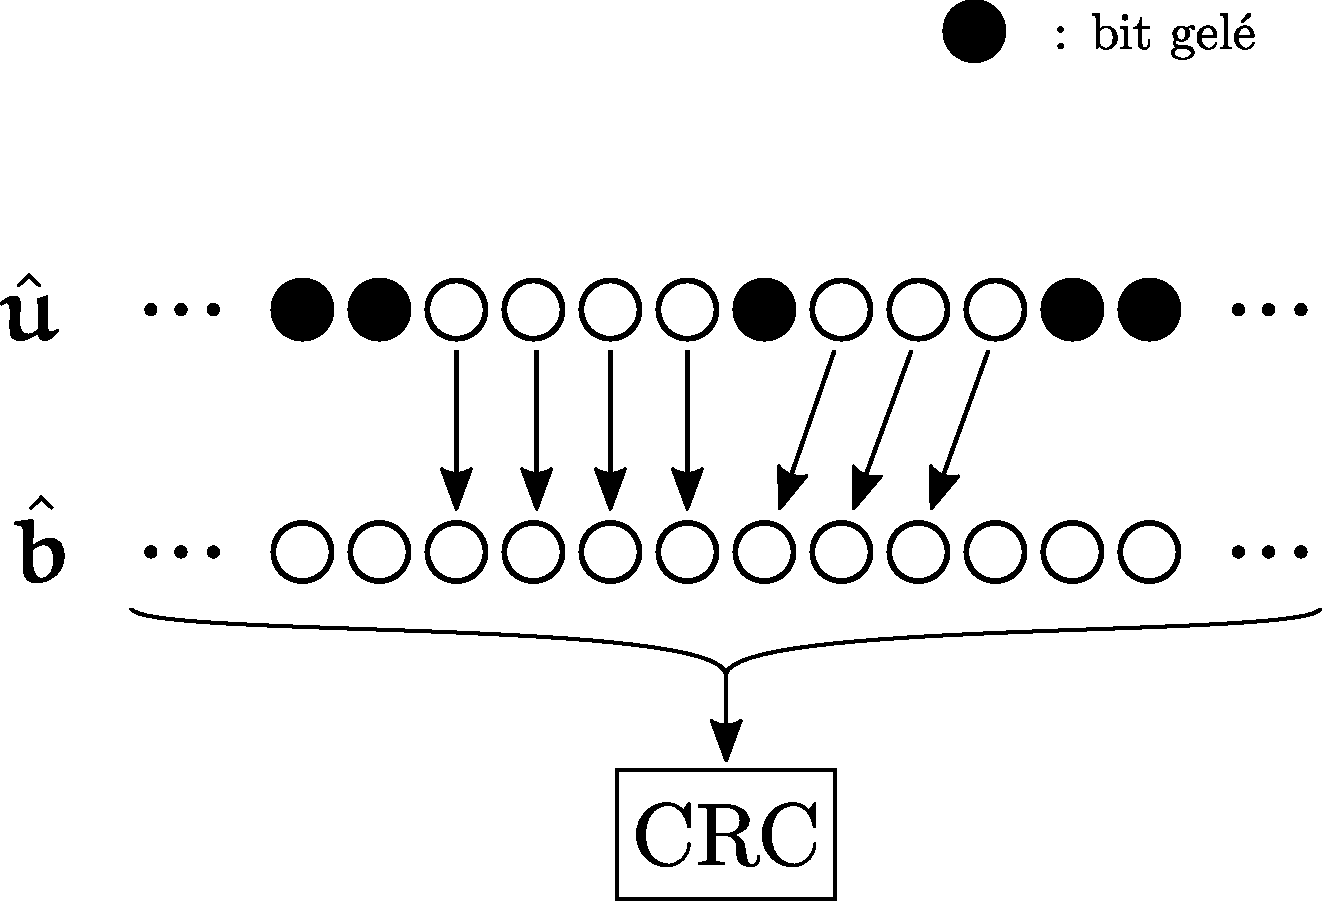
\includegraphics[height=120pt]{main/ch2_fig/extract1}
  \label{fig:extract1}
  }\quad
  \subfloat[Extraction parallèle]{
  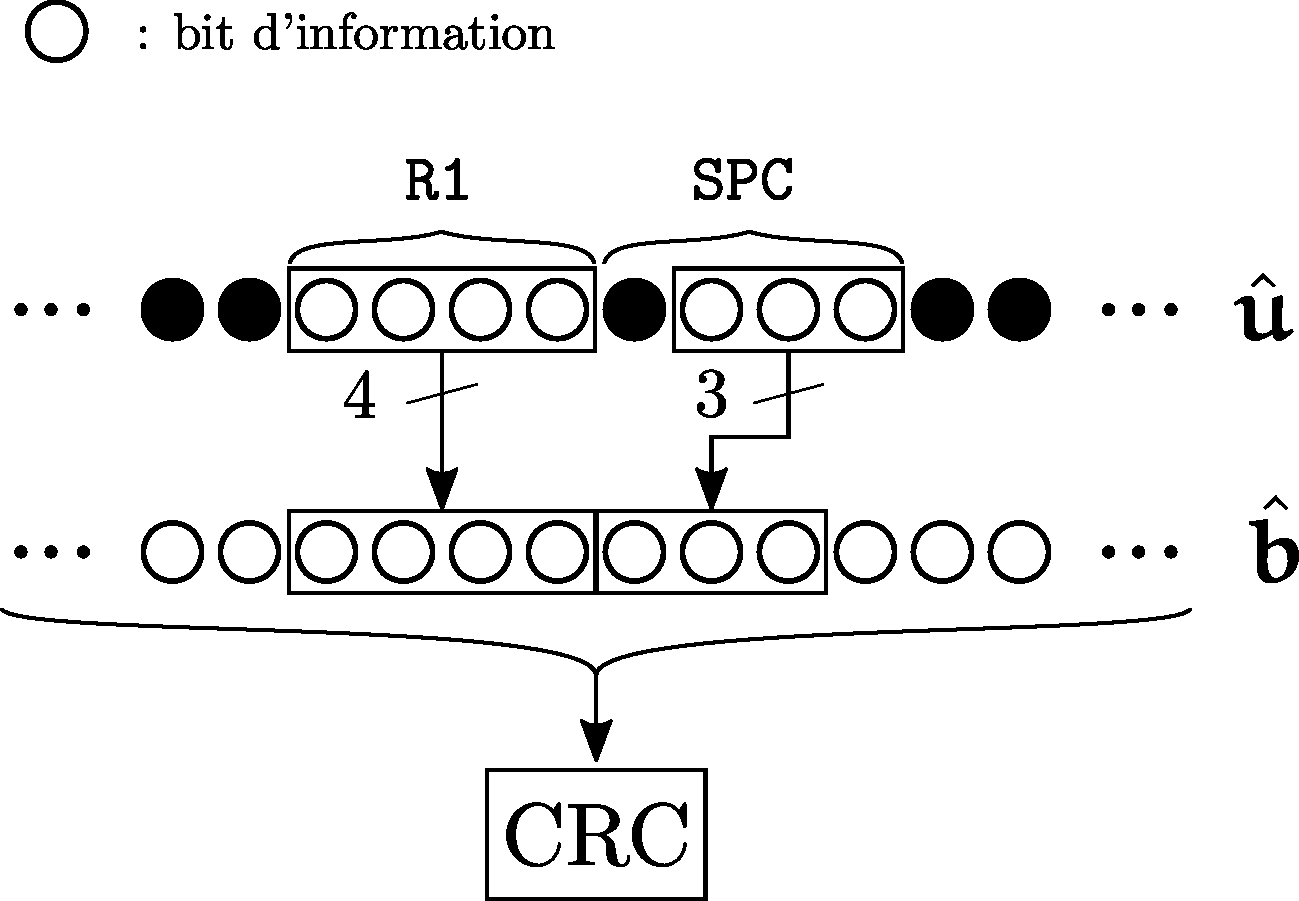
\includegraphics[height=120pt]{main/ch2_fig/extract2}
  \label{fig:extract2}
  }
  \caption{Extraction des bits d'information avant vérification du CRC}
  \label{fig:extract}
\end{figure}

Après chaque décodage SC ou SCL au sein des décodeurs adaptatifs, des mots de code candidats $\mathbold{\hat{u}}$ de $N$ bits sont produits.
Toutefois, le CRC est calculé sur les $K$ bits d'information de $\mathbold{\hat{b}}$ parmi les $N$ bits du mot de code.
Il est donc nécessaire de réaliser l'extraction des bits d'information.
L'implémentation naïve représentée dans la Figure~\ref{fig:extract1} consiste à réaliser cette extraction bit par bit.
Pour chaque bit, un test est réalisé pour savoir s'il s'agit d'un bit gelé ou d'un bit d'information.
Le profilage des décodeurs montre que cette opération d'extraction représente une portion non négligeable du temps total de traitement du CRC.
Or, il est possible de l'accélérer en utilisant l'emplacement des bits gelés et la connaissance des \noeuds d'élagage.
En effet, la présence d'un \noeud de type \texttt{R1} de taille $4$ correspond à la présence de $4$ bits d'information consécutifs dans le vecteur $\mathbold{\hat{u}}$ comme représenté en Figure~\ref{fig:extract2}.
La fonction (\texttt{std::copy}) de la bibliothèque standard C++ permet de réaliser une extraction parallèle de plusieurs bits.
Cette technique peut être étendue aux \noeuds \texttt{SPC} à condition d'exclure le bit gelé du \noeud en question.

Au cours de l'exécution des algorithmes adaptatifs, une vérification du CRC doit être effectuée une fois à la fin du décodage SC, et $L$ fois à la fin de chaque décodage SCL, afin de tester chaque candidat. En conséquence, l'accélération des vérifications de CRC est capital pour ces algorithmes adaptatifs.
Les mesures effectuées le vérifient. Pour l'algorithme FASCL sur un code polaire (2048,1723) associé un CRC de taille $c=32$ à $E_b/N_0 = 4.5dB$, le gain de performance d'exécution lié à l'utilisation des techniques présentées ci-dessus est de 63\%, portant le débit de 262 Mb/s à 426 Mb/s.

\subsection{Gestion des sommes partielles}
La gestion des sommes partielles dans les décodeurs proposés est détaillée dans cette sous-section.
Les sommes partielles sont des décisions dures. Cela signifie que leurs valeurs donc binaires. Cependant, dans les implémentations logicielles proposées, afin d'utiliser efficacement les instructions SIMD, les LLR et les sommes partielles sont stockés sur des entiers de même dimension, notée $Q$, en octets. Selon la représentation choisie, 32, 16 ou 8 bits, $Q$ peut donc prendre respectivement les valeurs 4, 2 ou 1. 
Dans les précédentes implémentations logicielles de l'algorithme SCL \cite{sarkis_fast_2016,sarkis_increasing_2014,shen_low-latency_2016}, un emplacement mémoire de $Q$ octets est alloué à chaque niveau de l'arbre de décodage comme décrit dans \cite{tal_list_2011}. La taille de l'emplacement mémoire associé à un niveau de l'arbre est égal à la taille des \noeuds du niveau en question. Soit $n=\log_2(N)$, le nombre total de niveaux est $n+1$ et la taille d'un \noeud au niveau $l$ est égale à $2^{n-l}$. L'empreinte mémoire pour les sommes partielles d'un arbre de décodage est, quant à elle, égale à : 
\begin{equation}
\sum^n_{l=0}2^{n-l}=2N-1
\end{equation}
Pour l'algorithme SCL dans lequel L arbres de décodage sont nécessaires, l'empreinte mémoire totale est donc $L(2N-1)$. Cependant, dans l'algorithme SC, les sommes partielles d'un \noeud donné de l'arbre de décodage ne sont utilisées qu'une seule fois au cours du décodage. Par conséquent, ces emplacements mémoire peuvent être réutilisés. Ainsi, l'empreinte mémoire est réduite de $2N-1$ à $N$ dans l'algorithme SC \cite{leroux_hardware_2011}. De même, il est possible de réduire cette empreinte mémoire de $L(2N-1)$ à $LN$ pour l'algorithme SCL.

Lors des étapes de duplication et de sélection de l'algorithme SCL, étapes $(i+1)$ et $(i+3)$ de la Figure \ref{fig:scl}, il est nécessaire d'affecter les sommes partielles d'un arbre de décodage original à un nouvel arbre. Deux méthodes sont envisageables pour réaliser cette affectation. La première, notée $SCL_{cpy}$, consiste à systématiquement copier les $N$ sommes partielles sauvegardées dans l'emplacement mémoire du premier arbre de décodage vers l'emplacement mémoire du second. La seconde, présentée dans \cite{tal_list_2011}, est de réaliser cette affectation à l'aide de pointeurs. Ainsi, tant que les sommes partielles de chaque arbre ne diffèrent pas, elles utilisent le même emplacement mémoire. Cette méthode est notée $SCL_{ptr}$.

\begin{figure}
\centering
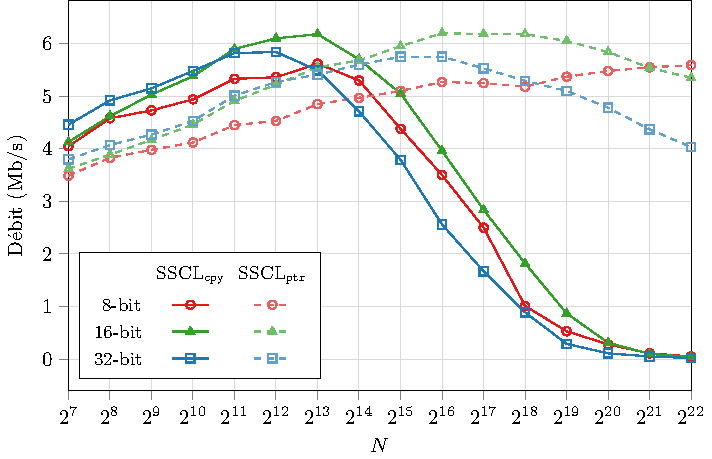
\includegraphics{main/ch2_fig/curves/thr/tikz/thr}
\caption{Comparaison des débits associés aux méthodes $SCL_{cpy}$ et $SCL_{ptr}$ pour différentes valeurs de $N$.}
\label{fig:scl_mem}
\end{figure}

La méthode $SCL_{ptr}$ semble plus efficace puisqu'elle évite des copies inutiles. Cependant, nos expérimentations ont montré que les calculs qui sont nécessaires à la gestion des pointeurs pénalisent cette méthode pour des codes de petite et moyenne tailles. La Figure~\ref{fig:scl_mem} représente les débits des implémentations de l'algorithme SCL associés aux deux méthodes, pour différentes valeurs de $N$, un rendement constant, $R=1/2$ et une profondeur de liste $L=32$. Ces courbes montrent que la méthode $SCL_{cpy}$ permet d'atteindre des débits plus élevés pour $N<8192$. En revanche, la méthode $SCL_{ptr}$ est plus avantageuse pour des tailles de codes supérieures. La Figure~\ref{fig:scl_mem} montre également l'impact du format utilisé pour la représentation des LLR et des sommes partielles. Pour de très grandes valeurs de $N$, la représentation sur 8 bits est plus efficace, puisqu'elle occupe moins d'espace mémoire et que les échecs d'accès à la mémoire cache sont plus rares. 

Trois optimisations originales permettant d'augmenter le débit et de réduire la latence des implémentations des algorithmes de décodage de codes polaire à liste sont détaillées dans la Section \ref{sec:opti_scl} : nouvel algorithme de tri, accélération du traitement du CRC, et nouvelle méthode de gestion des sommes partielles.




\section{Expérimentations : mesures et comparaisons}
\label{sec:exp_scl}

Les débits et les latences des implémentations proposées sont détaillées dans cette section. Tous les résultats proposés ont été obtenus grâce à l'outil AFF3CT \cite{aff3ct_aff3ct:_2016}. Le code source de ce logiciel est ouvert et disponible en ligne. Ainsi, tous les résultats sont facilement reproductibles. La cible matérielle est un CPU Intel i5-6600K d'architecture Skylake. Le jeu d'instruction SIMD AVX2 est exploité. Sa fréquence pour les résultats reportés est 3.9 GHz. La compilation a été effectuée sur un OS Linux avec le compilateur C++ de GNU (version 5.4.0). Les options de compilation qui ont été appliquées sont les suivantes : \texttt{-Ofast -march=native -funroll-loops}.

\subsection{Algorithme complètement adaptatif}
L'algorithme FASCL permet d'atteindre les débits les plus élevés. Comme il est montré dans le Tableau~\ref{tab:quantif}, l'implémentation de cet algorithme avec une représentation sur 8 bits des LLR et des sommes partielles permet d'atteindre un débit de 425 Mb/s pour un code polaire (2048,1723) et le CRC GZip de taille 32 bits lorsque $E_b/N_0=4.5dB$. Ce débit est pratiquement deux fois supérieur à celui obtenu avec l'algorithme PASCL. Le rapport signal à bruit pour lequel la différence entre PASCL et FASCL est la plus grande (380\%), est dans le domaine où le FER est compris entre $10^{-3}$ et $10^{-5}$. Il s'agit du domaine ciblé pour les communications sans fils comme le norme LTE ou le futur réseau 5G. Dans ces conditions, le débit de l'algorithme FASCL est d'approximativement 230Mb/s tandis que celui de PASCL est d'approximativement 40 Mb/s. Toutefois, rappelons que la latence dans le pire cas est plus élevée dans le cas de l'algorithme FASCL.

    \begin{table}[t]
      \centering
      \caption{Comparaison des débits et des latences des décodeurs proposés avec ceux de l'état de l'art. Représentation des LLR et sommes partielles sur 32 bits. Code polaire (2048,1723), $L=32$, CRC GZip $c=32$.}
      \label{tab:res}
      {\small\resizebox{\linewidth}{!}{
      \begin{tabular}{r|l|c|c|c c c}
        \multirow{2}{*}{\textbf{Cible}} & \multirow{2}{*}{\textbf{Algorithme}} & \multirow{2}{*}{\textbf{Version}}  & \multirow{1}{*}{\textbf{$\bm{\mathcal{L}_{PC}}$}} & \multicolumn{3}{c}{$\bm{\mathcal{T}_i}$ (Mb/s)} \\
        \cline{5-7}
        &                        &   & ($\mu s$)                          & \textbf{3.5 dB} & \textbf{4.0 dB} & \textbf{4.5 dB} \\
        \hline
        \parnoteclear
        i7-4790K & CASCL \parnote{{\footnotesize Version non élaguée de l'algorithme CASCL.}\label{pn:note}}  & \cite{shen_low-latency_2016}      & 1572                           & 1.10            & 1.10            & 1.10            \\
        \hline
        i7-2600  & CASCL\textsuperscript{1} & \cite{sarkis_increasing_2014}     & 23000                          & 0.07            & 0.07            & 0.07            \\
        i7-2600  & CASCL\textsuperscript{1} & \cite{sarkis_fast_2016}           & 2294                           & 0.76            & 0.76            & 0.76            \\
        i7-2600  & CASCL\textsuperscript{1} & Ce travail                        & 4819                           & 0.37            & 0.37            & 0.37            \\
        i5-6600K & CASCL\textsuperscript{1} & Ce travail                        & 3635                           & 0.48            & 0.48            & 0.48            \\
        \hline
        i7-2600  & CASCL & \cite{sarkis_increasing_2014}    & 3300                           & 0.52            & 0.52            & 0.52            \\
        i7-2600  & CASCL & \cite{sarkis_fast_2016}          & 433                            & 4.0             & 4.0             & 4.0             \\
        i7-2600  & CASCL & Ce travail                       & 770                            & 2.3             & 2.3             & 2.3             \\
        i5-6600K & CASCL & Ce travail                       & 577                            & 3.0             & 3.0             & 3.0             \\
        \hline
        i7-2600  & PASCL & \cite{sarkis_increasing_2014}    & $\approx$ 3300                 & 0.9             & 4.90            & 54.0            \\
        i7-2600  & PASCL & \cite{sarkis_fast_2016}          & $\approx$ 433                  & 8.6             & 33.0            & 196.0           \\
        i7-2600  & PASCL & Ce travail                       & 847                            & 5.5             & 31.1            & 168.4           \\
        i5-6600K & PASCL & Ce travail                       & 635                            & 7.6             & 42.1            & 237.6           \\
        \hline
        i7-2600  & FASCL & Ce travail                       & 1602                           & 19.4            & 149.0           & 244.3           \\
        i5-6600K & FASCL & Ce travail                       & 1201                           & 26.1            & 207.8           & 345.5           \\
      \end{tabular}
      }}
      \parnotes
    \end{table}

\subsection{Comparaison avec l'état de l'art}

Les débits et les latences des décodeurs proposés sont listés et comparés avec ceux de certains décodeurs de l'état de l'art dans le tableau \ref{tab:res}. Pour tous les décodeurs, les \noeuds SPC4+ ne sont pas utilisés afin de ne pas impacter les performances de décodage. La latence donnée dans le Tableau \ref{tab:res} est la latence \og pire cas \fg et le débit est le débit d'information moyen. La première version, CASCL, est l'implémentation de l'algorithme CASCL sans aucun élagage tandis que les versions notées CASSCL, FASSCL et PASSCL utilisent l'élagage de l'arbre. Le débit du décodeur CASSCL proposé (2.3 Mb/s) est seulement divisé par deux par comparaison avec l'implémentation spécifique déroulée de l'algorithme CASSCL décrite en \cite{sarkis_fast_2016} (4.0 Mb/s). Elle est approximativement 4 fois plus rapide que l'implémentation générique proposée en \cite{sarkis_increasing_2014} (0.52 Mb/s) et 2 fois plus rapide que celle proposée en \cite{shen_low-latency_2016}. Ce résultat est obtenu grâce aux améliorations algorithmiques proposées dans la section \ref{sec:opti_scl}. De plus, les implémentations proposées présentent une flexibilité et une généricité bien plus grandes que celles proposées dans \cite{sarkis_increasing_2014,shen_low-latency_2016}. En effet, les représentations quantifiées, la possibilité de définir des patrons de poinçonnage et la possibilité d'utiliser les algorithmes adaptatifs n'étaient pas offertes. En utilisant la même cible matérielle (i7-2600), l'implémentation de l'algorithme PASSCL présente des débits proches de l'implémentation spécifique déroulée de \cite{sarkis_fast_2016}. Enfin, le débit obtenu pour l'algorithme FASSCL est lui bien meilleur (jusqu'à 244 Mb/s pour $E_b/N_0=4.5dB$).

\subsubsection{Performances sur différentes cibles matérielles}
  \begin{table}[t]
    \centering
    \caption{Comparaison des débits, du nombre de cycles d'horloge nécessaires pour décoder une trame, et de l'énergie dépensée par bit décodé, pour des décodeurs proposés sur différentes cibles matérielles. Représentation en virgule fixe sur 8 bits , $E_b/N_0 = 4.5dB$, CRC GZip $c=32$.}
    \label{tab:port}
    {\small\resizebox{\linewidth}{!}{
    \begin{tabular}{r|c|c|c c c c| c c c| c c c}
      \multirow{3}{*}{\centering \textbf{Target}}  & \multirow{3}{*}{\begin{minipage}{0.5in}\centering \textbf{Freq. (MHz)}\end{minipage}} & \multirow{3}{*}{\centering \textbf{Algo.}}  & & \multicolumn{3}{c|}{$\bm{\mathcal{T}_i}$ \textbf{(Mb/s)}} & \multicolumn{3}{c|}{\textbf{\# Cycles par trame}} & \multicolumn{3}{c}{$\bm{\mathcal{E}_b}$ \textbf{(nJ/bit)}} \\
      \cline{4-13}
       & & & & \textbf{3.5} & \textbf{4.0} & \textbf{4.5} & \textbf{3.5} & \textbf{4.0} & \textbf{4.5} & \textbf{3.5} & \textbf{4.0} & \textbf{4.5} \\
       & & & & \textbf{dB}  & \textbf{dB}  & \textbf{dB}  & \textbf{dB}  & \textbf{dB}  & \textbf{dB}  & \textbf{dB}  & \textbf{dB}  & \textbf{dB}  \\
      \hline
      \hline
      \multirow{3}{*}{\begin{minipage}{0.5in}\centering i7 4790\end{minipage}}     & \multirow{3}{*}{\begin{minipage}{0.5in}\centering 3592\end{minipage}} 
        & CASCL &                     &  2.34  & 2.38   & 2.24   & 2645 & 2600 & 2763 & 6325 & 6218 & 6607 \\
      & & PASCL &                     &  5.80  & 33.88  & 207.96 & 1067 & 183  & 30   & 2552 & 437  & 71   \\
      & & FASCL &                     &  19.43 & 194.66 & 372.30 & 319  & 32   & 17   & 762  & 76   & 40   \\

      \hline
      \multirow{3}{*}{\begin{minipage}{0.5in}\centering Ryzen 2700X\end{minipage}} & \multirow{3}{*}{\begin{minipage}{0.5in}\centering 4230\end{minipage}} 
        & CASCL &                     &  2.68  & 2.72   & 2.56   & 2675 & 2635 & 2800 & 5149 & 5074 & 5391 \\
      & & PASCL &                     &  6.55  & 38.76  & 237.78 & 1094 & 185  & 30   & 2107 & 356  & 58   \\
      & & FASCL &                     &  20.93 & 209.37 & 406.15 & 342  & 34   & 18   & 659  & 66   & 34   \\

      \hline
      \multirow{3}{*}{\begin{minipage}{0.5in}\centering Cortex A73\end{minipage}} & \multirow{3}{*}{\begin{minipage}{0.5in}\centering 2360\end{minipage}} 
        & CASCL &                     &  1.23  & 1.28   & 1.20   & 3310 & 3175 & 3382 & 1475 & 1415 & 1507 \\
      & & PASCL &                     &  3.08  & 18.90  & 100.75 & 1319 & 215  & 40   & 588  & 96   & 18   \\
      & & FASCL &                     &  10.64 & 83.58  & 137.37 & 382  & 49   & 30   & 170  & 22   & 13   \\

      \hline
      \multirow{3}{*}{\begin{minipage}{0.5in}\centering Cortex A15\end{minipage}} & \multirow{3}{*}{\begin{minipage}{0.5in}\centering 2000\end{minipage}} 
        & CASCL &                     &  0.74  & 0.74   & 0.70   & 4639 & 4639 & 4923 & 3365 & 3365 & 3571 \\
      & & PASCL &                     &  1.81  & 11.06  & 61.86  & 1899 & 312  & 56   & 1378 & 226  & 40   \\
      & & FASCL &                     &  6.23  & 52.77  & 88.31  & 553  & 65   & 39   & 401  & 47   & 28   \\

      \hline
      \multirow{3}{*}{\begin{minipage}{0.5in}\centering Cortex A53\end{minipage}} & \multirow{3}{*}{\begin{minipage}{0.5in}\centering 1840\end{minipage}} 
        & CASCL &                     &  0.48  & 0.48   & 0.45   & 6560 & 6560 & 7064 & 1353 & 1353 & 1457 \\
      & & PASCL &                     &  1.17  & 7.32   & 42.77  & 2701 & 433  & 74   & 557  & 89   & 15   \\
      & & FASCL &                     &  4.45  & 39.70  & 68.32  & 712  & 80   & 46   & 147  & 16   & 10   \\

      \hline
      \multirow{3}{*}{\begin{minipage}{0.5in}\centering Cortex A7\end{minipage}} & \multirow{3}{*}{\begin{minipage}{0.5in}\centering 1400\end{minipage}} 
        & CASCL &                     &  0.28  & 0.29   & 0.27   & 8615 & 8318 & 8934 & 1071 & 1034 & 1111 \\
      & & PASCL &                     &  0.71  & 4.26   & 21.89  & 3397 & 566  & 110  & 423  & 70   & 14   \\
      & & FASCL &                     &  2.41  & 19.40  & 30.93  & 1001 & 124  & 78   & 124  & 15   & 10   \\

    \end{tabular}
    }}
  \end{table}

La description logicielle des décodeurs proposés est portable, grâce en particulier à l'utilisation du langage C++11 et de la bibliothèque MIPP \cite{cassagne2018mipp} pour ce qui concerne les instructions SIMD. Ainsi, en plus d'être efficace comme nous l'avons déjà vu sur des architectures de processeur de type x86, le décodeur bénéficie également d'optimisations pour l'exécution sur des processeurs du marché de l'électronique embarquée, à savoir des architectures ARM. Des résultats d'exécution sur plusieurs cibles sont récapitulés dans le Tableau~\ref{tab:port}. Les métriques prises en compte sont le débit d'information ($\bm{\mathcal{T}_i}$), le nombre de cycles d'horloge nécessaire pour décoder une trame et l'énergie dépensée par bit d'information décodé ($\bm{\mathcal{E}_b}$). Le Tableau~\ref{tab:port}  présente des résultats d'exécution sur un seul \coeur de processeur, sans utiliser le mode multifil simultané (SMT : Simultaneous MultiThreading).

Les deux premières cibles matérielles considérées sont deux processeurs à usage général pour station de travail, un Intel i7 4790 et un AMD Ryzen 2700X. Leurs architectures respectives sont de type x86-64 et tous deux possèdent les instructions SIMD AVX2. Les fréquences affichées sont celles mesurées au moment de l'exécution du programme, tout comme la puissance nécessaire pour le calcul de ($\bm{\mathcal{E}_b}$). Le logiciel utilisé pour ces mesures est HWiNFO \cite{noauthor_hwinfo_nodate}. La puissance mesurée est celle du \coeur de processeur seulement, excluant la consommation d'énergie de la mémoire principale et de la mémoire cache de niveau 3.

Par ailleurs, les résultats d'exécution des implémentations logicielles sur quatre versions différentes de processeurs ARM sont présentés. Les architectures ARM sont avantageuses du point de vue de la consommation énergétique pour l'algorithme de décodage SC \cite{cassagne_energy_2016}. Nous effectuons ici des mesures afin de vérifier que c'est aussi le cas pour l'algorithme SCL. Deux cartes d'évaluation ont été utilisées pour cela. La carte Hikey960 embarque la puce Kirin960 de Hisilicon. Il s'agit d'une puce à 8 \coeurs, 4 Cortex A73 et 4 Cortex A53 qui correspondent à la microarchitecture ARMv8-A. La valeur de puissance consommée n'est pas mesurée, car aucun capteur ne permet une telle mesure sur cette carte. Nous utilisons donc les valeurs de consommation données par le constructeur \cite{humrick_hisilicon_nodate}. La carte Odroid XU4 embarque la puce Samsung Exynos 5422 à 4 \coeurs Cortex A15 et 4 \coeurs Cortex A7 de microarchitecture ARMv7-A. La puissance considérée pour chacun des \coeurs est issue de \cite{holmgren_energy_nodate,benmoussa_performance_nodate}. Tous les \coeurs ARM possèdent le jeu d'instruction SIMD NEON.

Grâce à une fréquence de fonctionnement plus élevée, les processeurs de station de travail atteignent de plus hauts débits que les processeurs ARM. Nous observons également que malgré des fréquences de fonctionnement proches, le Cortex A73 présente un débit bien plus important que le Cortex A15. Cela est sans doute lié au changement de microarchitecture entre les deux générations. En effet, il y a une diminution d'environ 30\% du nombre de cycles nécessaires pour décoder une trame. Un écart du même ordre de grandeur est observé entre les Cortex A53 et A7, qui sont des \coeurs à faible consommation énergétique.

Du point de vue du nombre de cycles d'horloge nécessaires au décodage d'une trame, il est important d'observer que le Cortex A73 est compétitif par rapport aux processeurs de station de travail, le i7 et le Ryzen. En conséquence, puisque sa puissance est bien inférieure ($\approx 2 W$ en charge contre $\approx 15 W$), l'efficacité énergétique est elle 3 à 4 fois supérieure. Les Cortex A7 et A53 sont proches en termes d'efficacité énergétique tandis que le Cortex A15 s'avère être en retrait.



\section{Conclusion}

L'infrastructure Cloud-RAN et plus généralement l'attrait grandissant pour le domaine des radios logicielles (SDR : Software Defined Radio) motivent l'étude et le développement de descriptions logicielles de décodeurs canal comme celles décrites dans ce chapitre.

Voici résumées les différentes contributions originales proposées.
\begin{enumerate}[label=(\roman*)]
  \item Au contraire des implémentations des algorithmes à liste logicielles précédentes, celles-ci sont les premières à permettre une représentation en virgule fixe sur une nombre réduit de bits des LLR.
  \item Deux méthodes différentes de gestion des sommes partielles sont présentées. Leurs avantages et inconvénients sont étudiés.
  \item Une méthode d'extraction des bits d'information, nécessaire avant les vérifications de CRC dans les différents algorithmes, est présentée. Elle permet d'augmenter significativement le débit des décodeurs.
  \item Un algorithme de tri \cite{schreier_tournament_1932} très adapté aux algorithmes considérés est utilisé pour la première fois.
  \item Contrairement aux implémentations à haut débit et faible latence proposées dans les travaux précédents, les décodeurs proposés supportent l'algorithme FASCL.
  \item Un type d'élagage était présenté dans des travaux précédents comme dégradant fortement les performances de décodage. Le paramétrage fin de l'élagage dans les décodeurs proposés a permis de montrer que ce fait est discutable suivant le code polaire considéré.
  \item Les implémentations sur architecture ARM des algorithmes de décodage de codes polaires à liste sont les premières de la littérature.
\end{enumerate}
Ces contributions ont fait l'objet d'un article en cours de revue \citemine{leonardon_fast_2017} pour publication dans le \textit{Journal of Signal Processing Systems}.


Des architectures programmables permettant l'implémentation efficace d'algorithmes de décodage de codes polaires sont détaillées dans la suite de ce manuscrit. L'objectif recherché est de conserver  la souplesse et la flexibilité apportée par une description logicielle des algorithmes de décodage, tout en améliorant le débit, la latence, et surtout l'efficacité énergétique des décodeurs résultants.             % Second thème (Doctorat) ou "Résultats théoriques et expérimentaux" (Maîtrise).
%!TEX root = ../my_thesis.tex
\chapter{Processeurs personnalisés à faible consommation pour le décodage SC} % (fold)
\label{chap:tensilica}

\vspace*{\fill}
\minitocTITI
\vspace*{\fill}
\newpage

\section*{Introduction}
Les implémentations logicielles des fonctions de traitement du signal dans les infrastructures de communication radio sont encouragées pour tendre vers un réseau virtualisé de type Cloud-RAN. De telles implémentations sont présentées pour les algorithmes de décodage polaire à liste dans le chapitre précédent. De hauts débits peuvent être atteints, et la flexibilité et la généricité de ces décodeurs est très importante. En utilisant des processeurs visant des systèmes électroniques embarqués, ces implémentations peuvent également gagner en efficacité énergétique.

Toutefois, les processeurs à usage général incluent de nombreuses unités matérielles destinées à réaliser efficacement de nombreuses et diverses applications. Mais ces unités matérielles ne sont pas utilisées dans certaines de ces applications. Par exemple, dans les algorithmes de décodage de canal, toutes les unités de calcul à point flottant sont inutiles puisqu'une représentation des données interne par virgule fixe est suffisante. Ces unités matérielles consomment de l'énergie inutilement. Le profilage d'un décodeur polaire montre que la majeure partie du temps d'exécution est passé à réaliser un ensemble restreint de fonctions élémentaires. De plus, une part significative des instructions exécutées correspond à des opérations de sauvegarde et de chargement de données dans les registres.

Ces observations poussent à envisager la conception d'un processeur programmable qui exclurait les unités matérielles inutiles des processeurs à usage général, tout en intégrant des unités de calculs spécialisées dans la réalisation efficace des fonctions élémentaires de décodage de codes polaires. Ce type de processeurs entre dans la catégorie des processeurs à jeu d'instructions spécifique à l'application (ASIP: Application Specific Instruction-set Processor).

Les Chapitres \ref{chap:tensilica} et \ref{chap:tta} de ce manuscrit présentent deux architectures de processeurs ASIP spécialisées dans le décodage de code polaire. Ces deux architectures ont été conçues selon des méthodologies de conception différentes. Dans la section \ref{sec:asips}, le concept d'ASIP est introduit, et la méthodologie utilisée pour la première architecture est décrite. Dans la section \ref{tensilica_design}, la conception de l'ASIP est détaillée. Enfin les résultats d'implémentation et les performances de l'architecture en termes de débit, latence, complexité et consommation énergétiques sont présentés et discutés dans la section \ref{sec:tensilica_res}.


\section{Les processeurs à jeu d'instructions spécifique à l'application}
\label{sec:asips}

L'architecture ASIP que nous avons développée est basée sur une processeur de type RISC (Reduced Instruction Set Computer). Dans une première sous-section, les principes des architectures RISC sont présentés. Le concept d'ASIP sera ensuite introduit ainsi que leurs deux grandes méthodologies de conception. Le flot de conception de l'outil logiciel utilisé pour concevoir notre ASIP sera ensuite présenté.

\subsection{Les processeurs RISC}
\label{subsec:risc}
\begin{figure}[t]
\centering
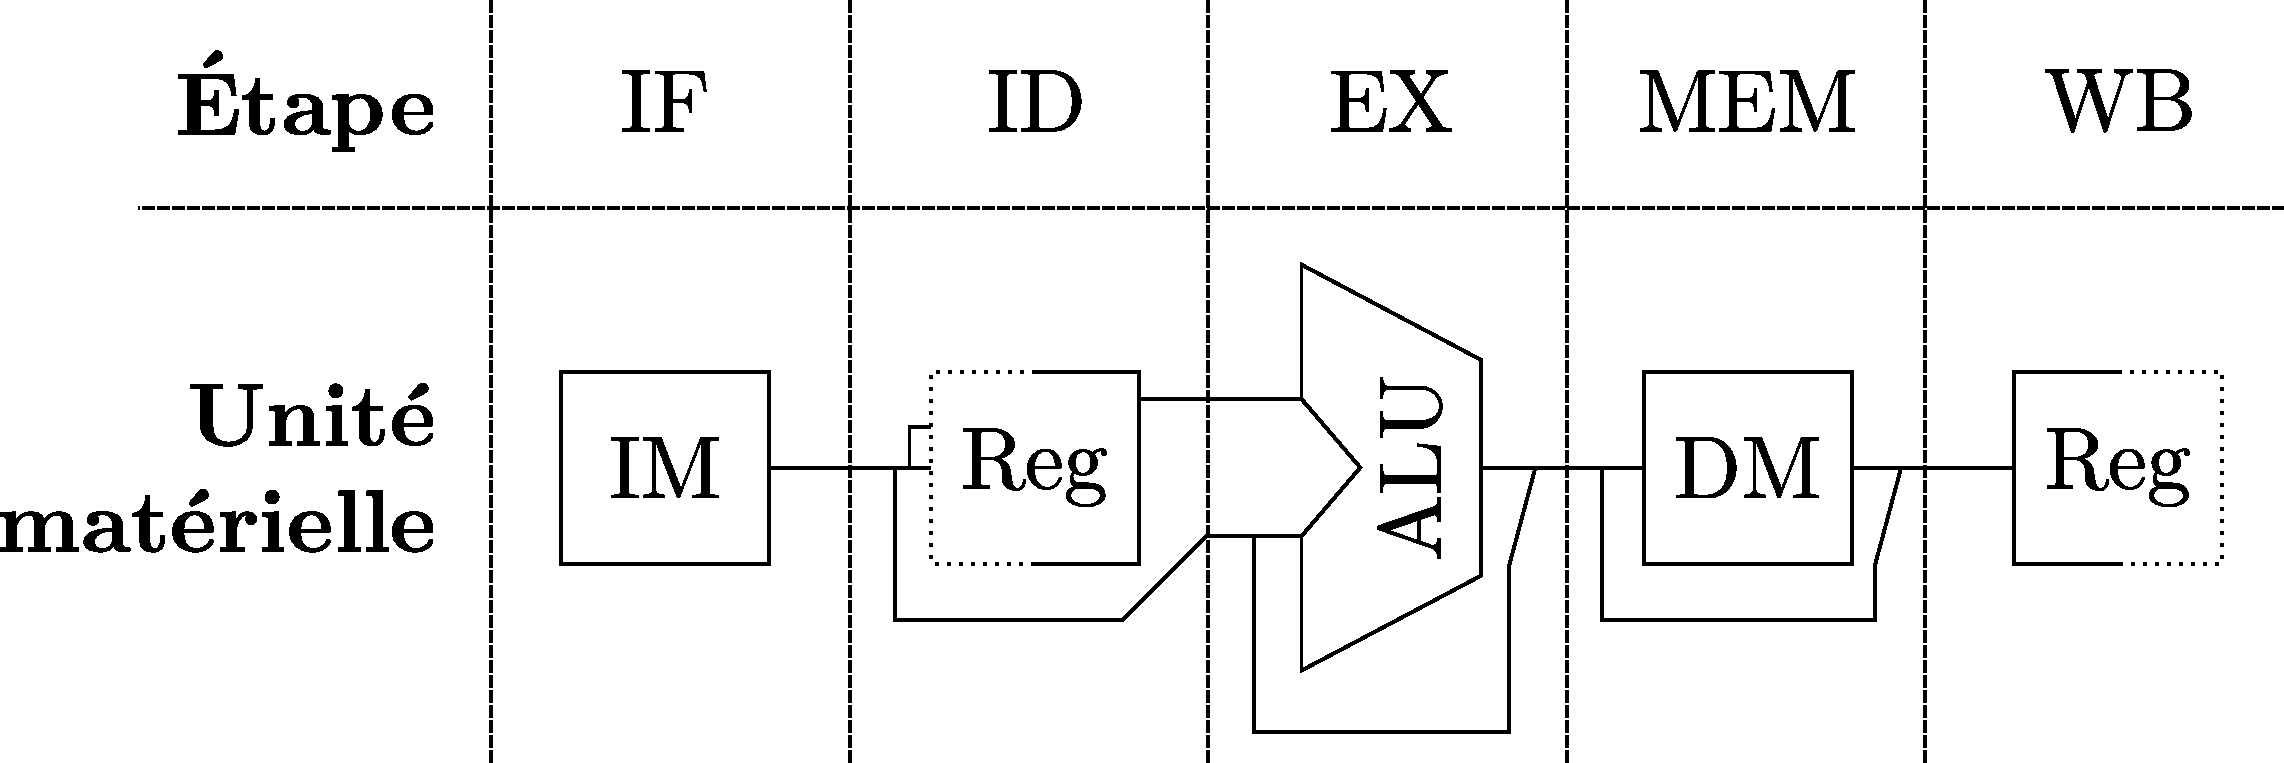
\includegraphics[width=\textwidth]{main/ch3_fig/stages}
\caption{\'Etages d'un processeur RISC}
\label{fig:risc}
\end{figure}

Dans le domaine de l'embarqué, les processeurs utilisés sont souvent de type RISC. Cette classe de processeurs a été introduite dans \cite{hennessy2011computer}. Par une analyse statistique et quantitative des applications traitées par les architectures de processeurs, les auteurs ont abouti à une microarchitecture de processeurs composée de 5 étages. Une unité matérielle est associée à chacun des étages, comme montré dans la figure \ref{fig:stages}.

\begin{itemize}
  \item Le premier étage est l'étage de \textbf{chargement de l'instruction} (IF : Instruction Fetch) depuis la \textit{mémoire d'instruction} (IM : Instruction Memory). A chaque coup d'horloge, une nouvelle instruction est chargée dans un registre spécialisé, nommé registre d'instruction. L'adresse en mémoire de l'instruction à lire est déterminée par le pointeur d'instruction, registre incrémenté automatiquement à chaque coup d'horloge. L'instruction contient l'opération qui sera effectuée par le processeur dans les étages suivants. Il peut s'agir d'instructions arithmétiques et logiques, d'instructions de chargement et de sauvegarde depuis et vers la mémoire, ou bien d'instructions de branchement et de sauts, afin de se déplacer dans la mémoire d'instructions. Elle contient également des informations sur les registres qui doivent être lus ou écrits, ainsi que des adresses mémoire dans le cas d'opérations de chargement ou de sauvegarde.

  \item Le deuxième étage est le \textbf{décodage de l'instruction} (ID : Instruction Decode) et de lecture du \textit{fichier de registre} (RF : Register File) spécifié(s) par l'instruction. Divers signaux de contrôle, qui seront utilisés dans les étages suivants, sont générés, selon l'instruction décodée.

  \item Le troisième étage est l'étage d'\textbf{exécution} (EX : Execution) dans lequel l'unité arithmétique et logique (ALU : Arithmetical and Logical Unit) effectue des opérations arithmétiques (+,-,*,/) et logiques (AND, OR, XOR,...). Ces opérations peuvent servir a effectué des calculs d'adresse relative ou a réaliser des opérations sur deux entrées. Ces deux entrées peuvent être deux registres ou bien un registre et une valeur immédiate intégrée dans l'instruction elle-même.

  \item Le quatrième étage est l'étage d'\textbf{accès à la mémoire}. S'il s'agit d'un chargement, une donnée est lue dans la \textit{mémoire de donnée} (DM : Data Memory) à l'adresse spécifiée par un des registres. S'il s'agit d'une sauvegarde, la valeur d'un deuxième registre est écrite dans la DM.

  \item Le cinquième est l'étape d'\textbf{écriture différée} (WB : write-back). Cette étage permet d'écrire le résultat dans le fichier de registre, que ce soit le résultat d'une opération effectuée par l'ALU ou bien une donnée lue dans la DM.
\end{itemize}

\begin{figure}[t]
\centering
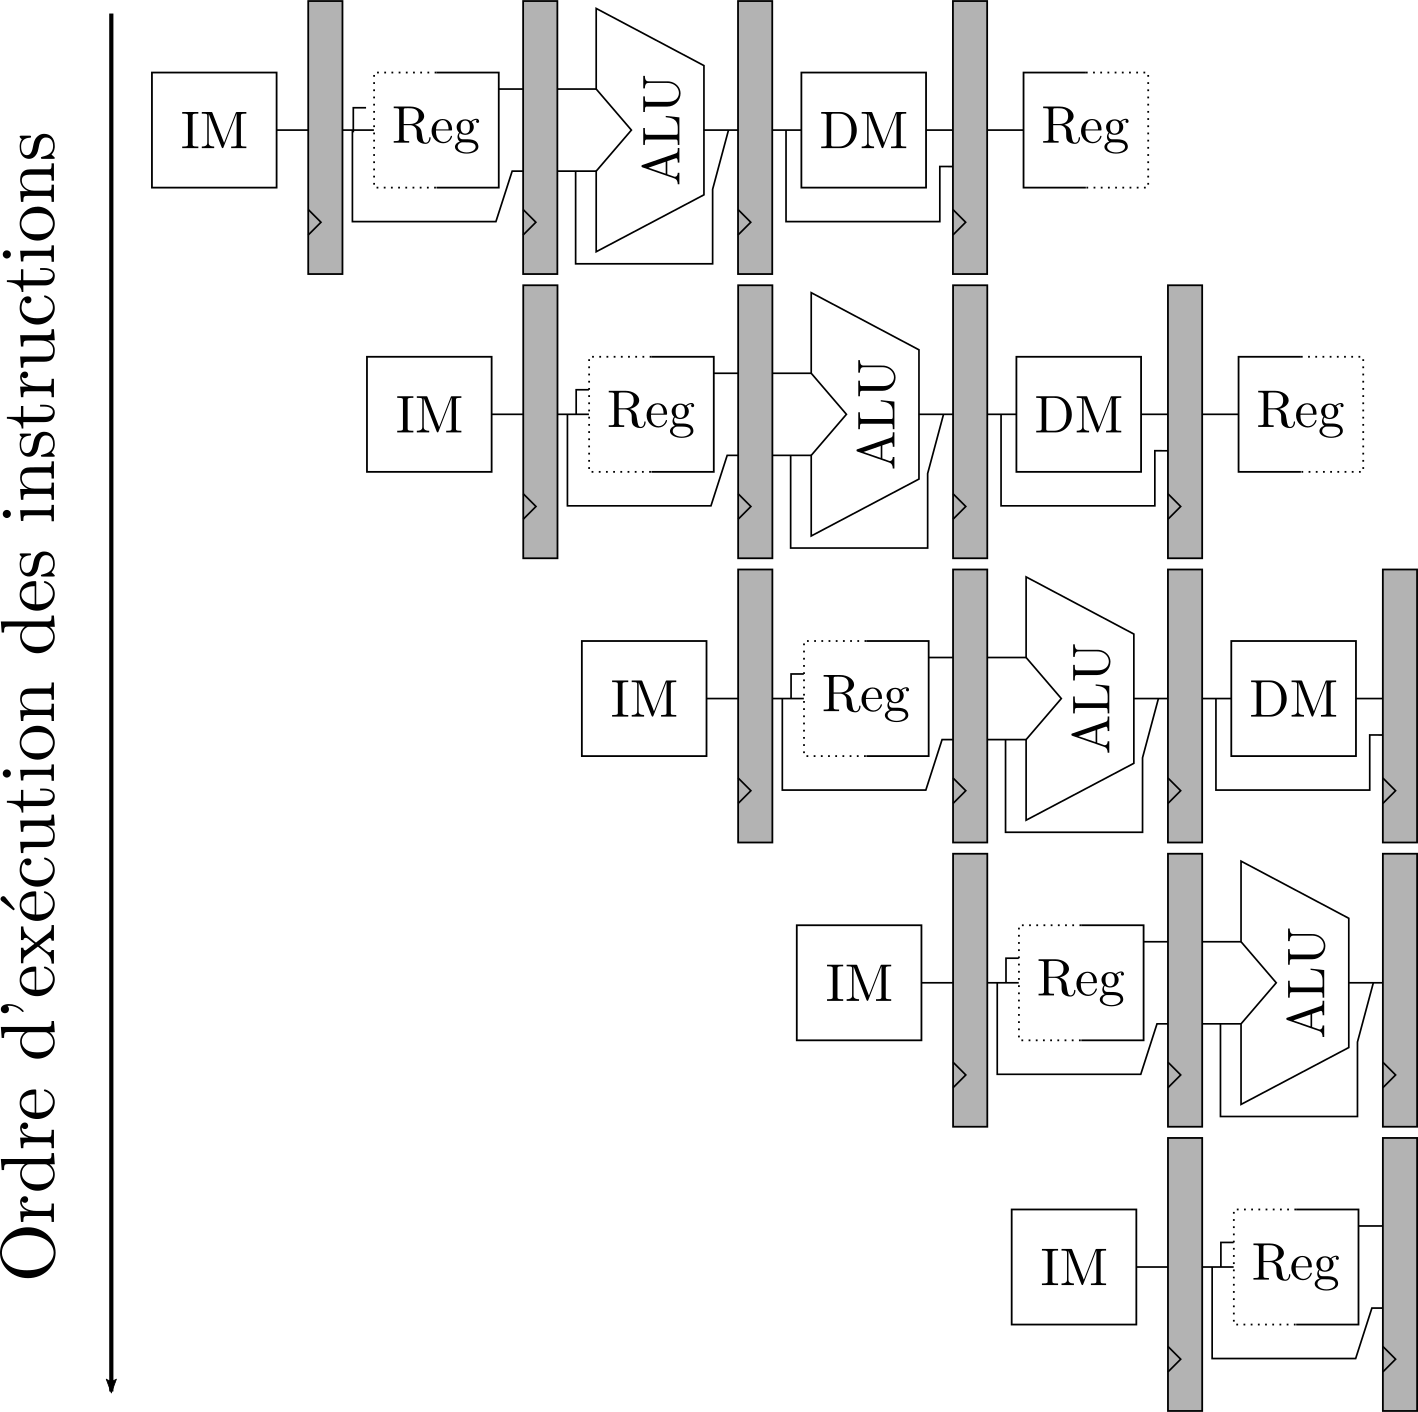
\includegraphics[width=0.75\textwidth]{main/ch3_fig/pipelines}
\caption{Pipeline à 5 étages}
\label{fig:pipelines}
\end{figure}


L'ajout de registres de pipeline représentés dans la Figure~\ref{fig:pipelines} permet d'isoler chacun des étages. Ainsi à chaque cycle d'horloge, représenté ici par les lignes horizontales, une instruction est transmise d'un étage au suivant. Si une instruction est initiée à chaque coup d'horloge, alors la performance du processeur sera 5 fois supérieure à celle d'un processeur sans registre de pipeline.

Voici donc les grandes lignes de l'architecture RISC définie dans \cite{hennessy2011computer} et qui fait figure de référence dans le domaine. En effet, ce même pipeline à cinq étages, à quelques différences près mais dont la structure est proche, se retrouve dans de nombreux processeurs du marché. L'architecture de base des processeurs Tensilica proposés dans ce chapitre est une architecture de type RISC.

\subsection{Les processeurs à jeu d'instructions spécifique à l'application}

Les méthodologies de conception des ASIP peuvent être divisées en deux famille. La première famille correspond à un flot de conception basé sur la spécification complète du processeur, représentée dans la Figure \ref{fig:methodo_adl}. Le modèle du processeur est décrit dans un langage de description architectural (ADL : Architecture Description Language) \cite{mishra2011processor}. Ces langages de description permettent de définir précisément l'architecture d'un processeur. Ils peuvent être de différents types. Les ADLs structurels décrivent les composants des processeurs ainsi que leurs interconnexions. Les ADLs comportementaux décrivent quand à eux le comportement du jeu d'instructions du processeur. Des langages de description mixtes permettent quant à eux de décrire simultanément la structure et le comportement du langage. Le flot de conception utilisé pour concevoir le processeur décrit dans le Chapitre \ref{chap:tta} utilise de tels langages de description afin de générer le modèle matériel du processeur.


\begin{figure}[]
  \centering
  \subfloat[Flot basé sur la spécification complète du processeur.]{
  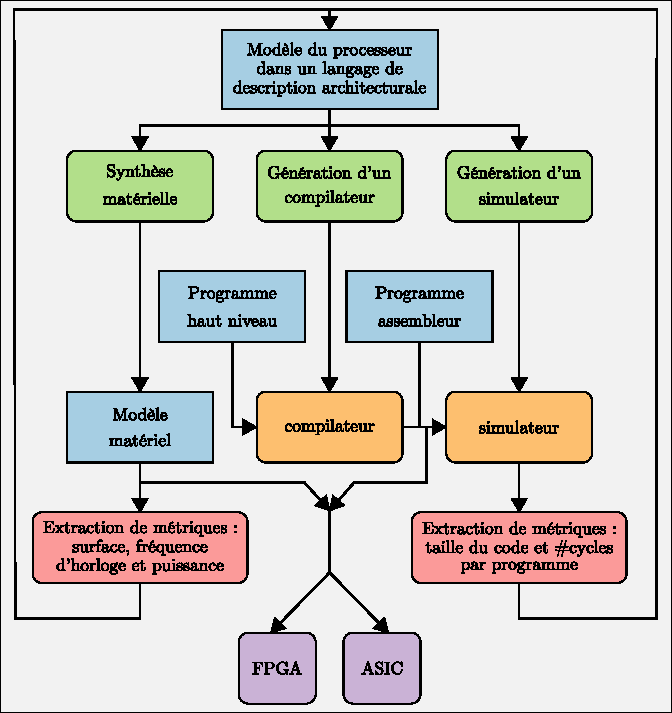
\includegraphics[scale=0.83]{main/ch3_fig/methodo_a}
  \label{fig:methodo_adl}
  }
  \\
  \subfloat[Flot basé sur la particularisation d’un processeur de base]{
  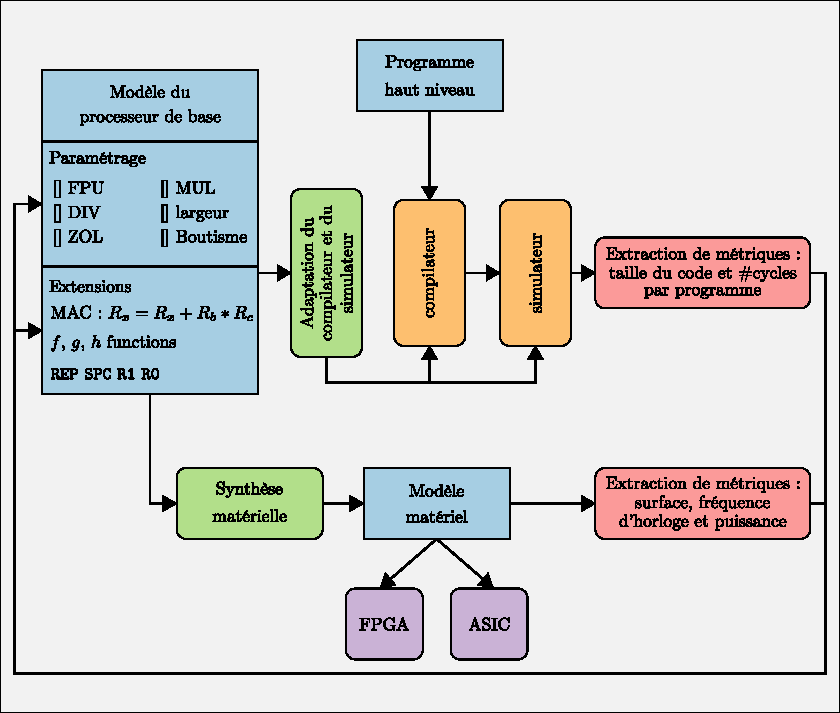
\includegraphics[scale=0.83]{main/ch3_fig/methodo_b}
  \label{fig:methodo_tensilica}
  }
  \caption{Méthodologies de conception des ASIP}
  \label{fig:asip_methods}
\end{figure}


La deuxième famille de méthodologies représentée dans la Figure \ref{fig:methodo_tensilica} correspond à l'approche utilisée par les outils Tensilica, utilisés pour concevoir l'ASIP proposé dans ce chapitre. Une architecture de base, peu complexe en terme d'aire occupée et à faible consommation constitue la brique de base du processeur. Dans le cas des outils Tensilica, l'architecture de base est un processeur RISC doté d'un pipeline de 5 étages tels que présenté dans la sous-section \ref{subsec:risc}. Afin de spécialiser le processeur, deux axes de de conception sont disponibles. Premièrement, le pipeline de base, dont les principales unités matérielles ont été désignées dans la figure \ref{fig:risc} sont paramétrable. Leurs caractéristiques (profondeur et largeur de la file de registre, intergace avec les mémoires...) sont modifiables. Des fonctions peuvent être ajoutées ou enlevées, comme il est montré en Figure \ref{fig:methodo_tensilica} : unité de traitement des points flottants (FPU : Floating Point Unit) unité d'accélération des multiplications (MUL) ou des divisions (DIV)... Le deuxième axe est la possibilité d'étendre le jeu d'instructions. Grâce à un langage de description matériel propre à Tensilica (TIE : Tensilica Instruction Extension) \cite{tie2017reference}. Il est possible dans notre cas d'un processeur spécialisé dans le décodage de codes polaires d'ajouter des unités matérielles accélérant les fonctions élémentaires $f$, $g$, $h$.

Un des objectifs de la conception de processeurs par les méthodologies des conceptions que nous venons de présenter est de réduire de temps de mise sur le marché des systèmes conçus. Pour cela, des étapes clés pour la conception des processeurs sont automatisées. En effet, les suites logicielles de conception d'ASIPs permettent la génération automatique du compilateur, du simulateur, d'un outil de profilage et d'un outil de débogage. 

La génération du compilateur est critique. En effet, l'effort à déployer pour créer un compilateur associé à un processeur spécifique est considérable. En revanche, les compilateurs associés aux outils de conception d'ASIPs sont \og reciblables \fg. Ils sont capables de s'adapter à des modifications de l'architecture du processeurs. Un bon compilateur saura s'adapter aux changements de structure du processeurs et proposer des optimisations spécifiques à la structure. Il doit également être capable de s'adapter au nombre de registres, et de les utiliser efficacement. Nous verrons dans le cas de notre processeur spécialisé dans le décodage de codes polaires que l'augmentation du nombre de registres à usage général augmentera le débit de décodage. Le compilateur doit également être capable de gérer des modifications du pipeline et de permettre du parallélisme d'instructions.

Le simulateur et le profileur générés permettent la validation fonctionnelle de l'architecture et du programme associé. Le nombre de cycles nécessaires à l'exécution du programme est obtenue grâce au simulateur. Le profileur donne des informations importantes sur la durée de l'exécution de sous-parties du programme afin de cibler les sections les plus consommatrices de temps. Ces métriques déterminent les modifications futures à apporter pour créer un nouveau modèle du processeur. L'outil de conceptions d'ASIP générera alors de nouveaux compilateur, simulateur et profileur pour extraire les nouvelles métriques. Des itérations successives de ce flot permettent d'améliorer progressivement les performances de l'architecture et du programme considérés. Ce processus serait difficilement réalisable sans une telle suite d'outils automatisés.

Une fois l'architecture du processeur déterminée, le modèle matériel du processeur est généré. Ce modèle matériel peut être synthétisé et implémenté sur différentes cibles, ASIC ou FPGA. Il est alors possible d'extraire les métriques d'implémentations : fréquence de fonctionnement, surface occupée, puissance consommée. De nouveau, des itérations sont possibles afin d'améliorer progressivement les performances.
Pour le processeur Tensilica conçu dans le cadre de cette étude, la génération du modèle matériel n'a pas été possible par défaut de licence suffisante de l'outil de conception d'ASIPs. Seules des estimations de fréquences, de surface et de puissance sont produites par l'outil. Cette absence de modèle matériel a été une des raisons pour lesquelles nous avons cherché à utiliser par la suite d'autres méthodologies de conception telles que celle décrite dans le Chapitre \ref{chap:tta}.

\section{Un ASIP dédié au décodage de codes polaires}
\label{subsec:sota_sc}
\subsection{Paramétrage du processeur de base}
\subsubsection{Architecture de base}
La philosophie de conception de l'ASIP proposé est de réaliser l'ensemble des fonctions élémentaires polaires à l'aide d'unités matérielles spécialisées, tandis que les opérations de contrôle sont effectuées par les unités matérielles de base du processeur XTensa. Ce processeur de base est donc dépourvu de tout accélérateur matériel de calcul. Il n'y a pas d'unité de calcul flottant, d'unité MAC (Multiple and Accumulate), d'unité accélérant les divisions ou les multiplications.

\begin{figure}
\centering
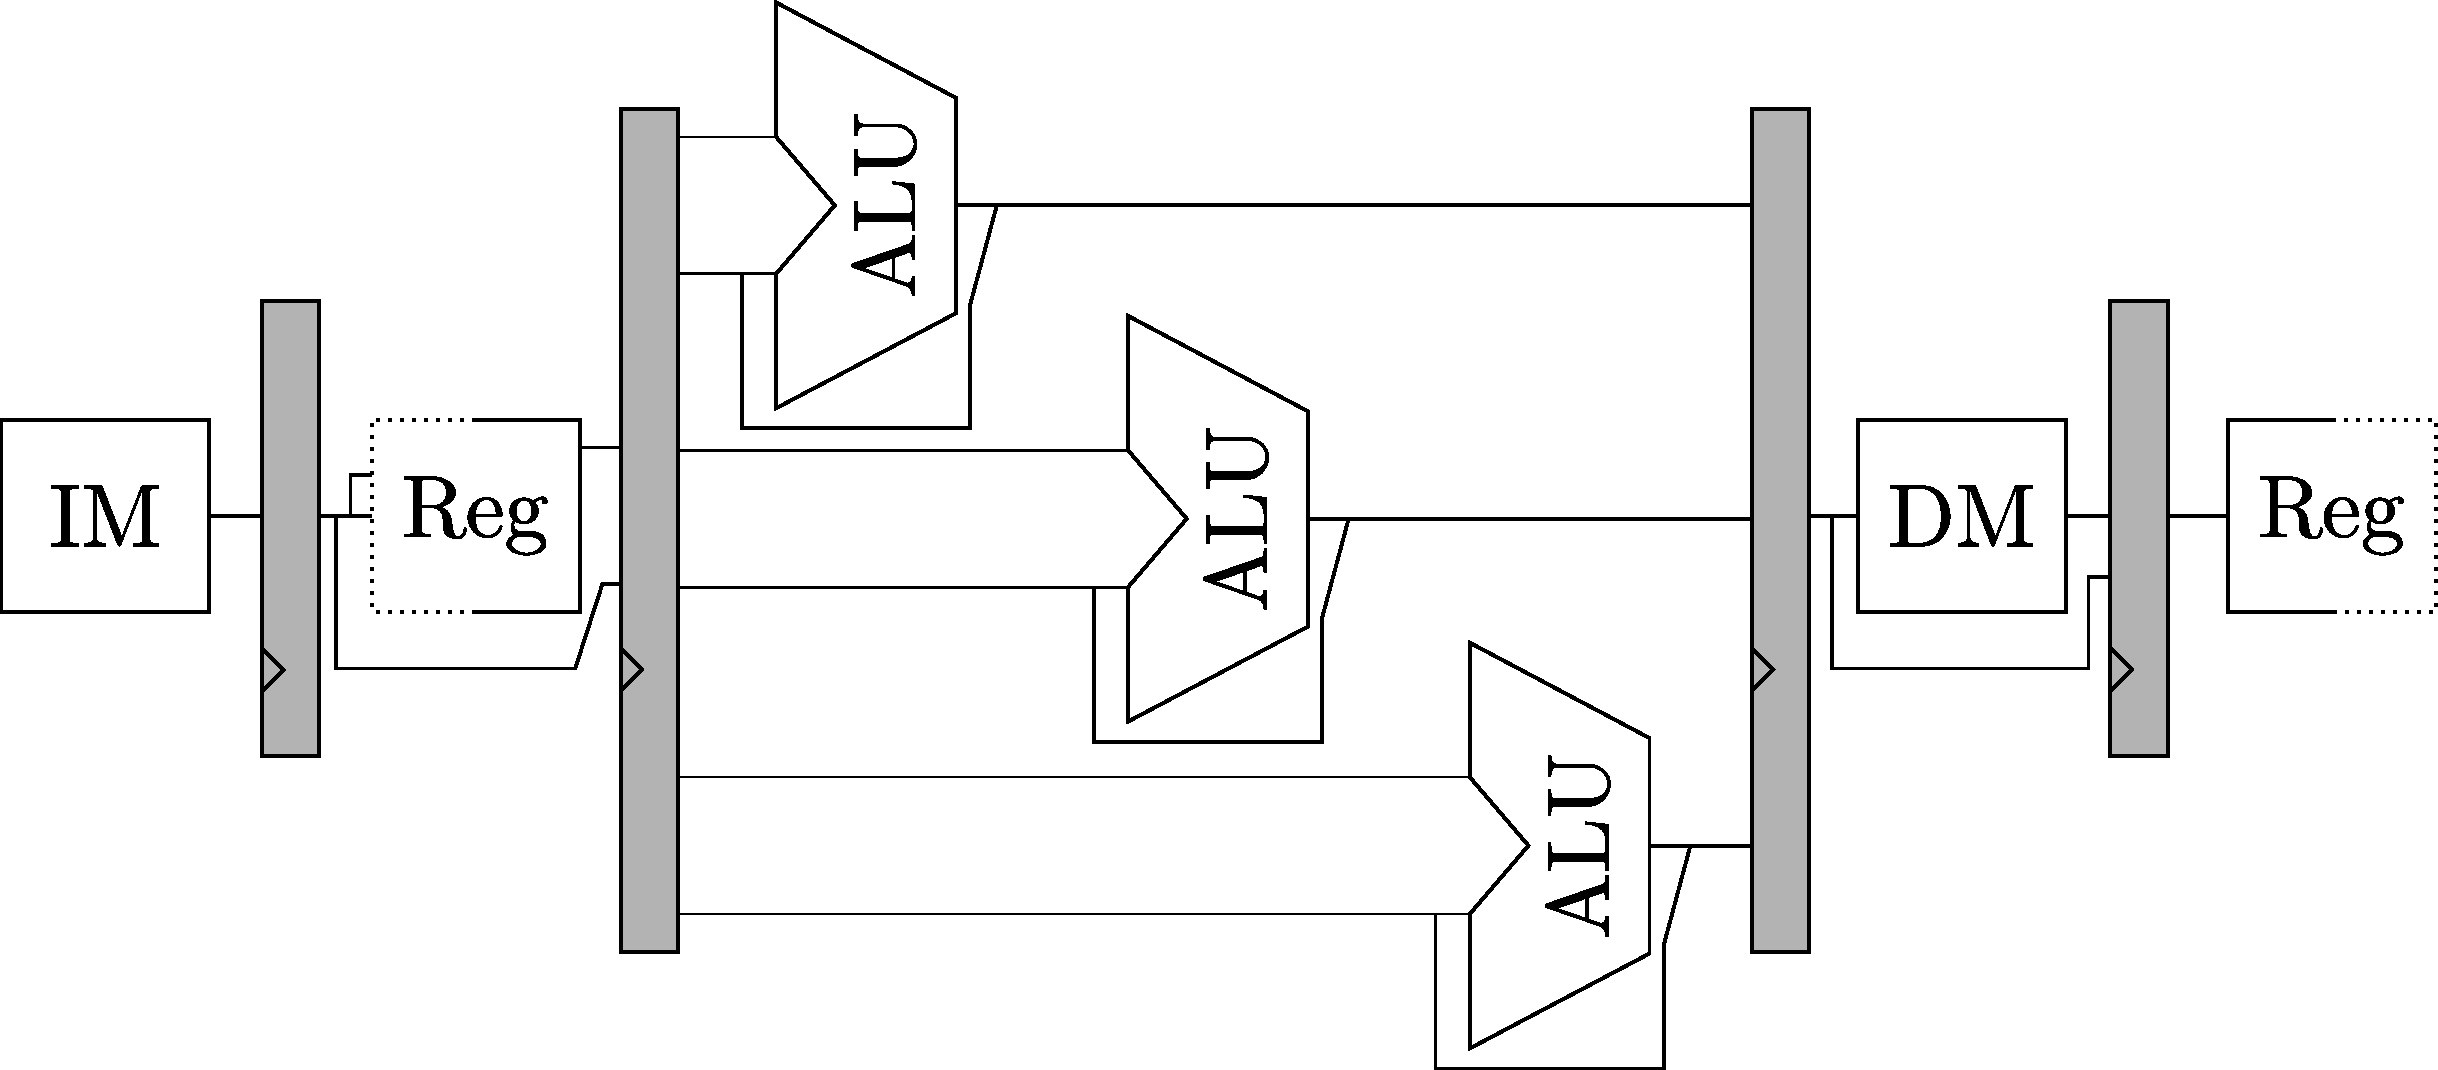
\includegraphics[width=\textwidth]{main/ch3_fig/flix}
\caption{Fonctionnalité FLIX.}
\label{fig:flix}
\end{figure}

La fonctionnalité FLIX de Tensilica correspond à la possibilité d'ajouter des ALUs supplémentaires au pipeline principal. Cela permet au processeur d'exécuter plusieurs instructions en parallèle. Il est possible de configurer les instructions réalisées par chaque pipeline. Notre choix s'est porté sur une configuration nommée FLIX3 prédéfinie par l'outil de conception. Ainsi, trois instructions faisant partie du jeu d'instruction de base peuvent être appliquées sur trois données de 32 bits simultanément. Ce parallélisme d'instructions permet de réaliser plus rapidement les fonctions de contrôle et de calcul d'adresse. La fonctionnalité FLIX est représentée en Figure \ref{fig:flix}.
La profondeur du fichier de registre a été augmentée de 32 à 64 données de 32 bits. En effet cela permet de tirer meilleure partie de l'augmentation du parallélisme d'instructions.

\subsubsection{Quantification des données}
Il est démontré dans \cite{sarkis_fast_2014} que des LLRs représentés sur 6 bits permettent d'égaler les performances de décodage d'implémentations en virgule flottante. Cependant, il est plus simple dans une implémentation logicielle de représenter ces données sur 8 bits puisque les langages de programmation définisse de tels types de données. Comme montré dans \cite{leroux_hardware_2011}, à un niveau $d$ de l'arbre de décodage doivent être stockés $2^{n-d}$ LLRs. La taille de la mémoire permettant de stocker les LLRs est donc de $2^{n+1}-1$ octets.

Les sommes partielles sont des valeurs binaires. Cependant, encore une fois, la manipulation des sommes partielles dans le langage de description logicielle est plus aisée si l'on utilise un entier de 8 bits pour représenter chaque somme partielle. Il serait cependant possible d'utiliser un entier pour représenter 8 sommes partielles, ce qui réduirait l'empreinte mémoire de celles-ci. Cela nécessiterait cependant des opérations de masquage supplémentaires et plus d'irrégularités dans les accès aux données.

\subsubsection{Configuration de la mémoire cache}
\begin{figure}
\centering
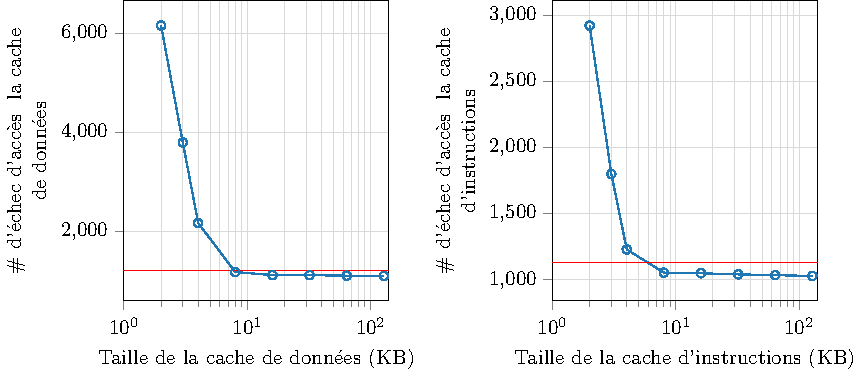
\includegraphics[width=\textwidth]{main/ch3_fig/curves/memory/tikz/memory}
\caption{Nombre d'échecs d'accès à la mémoire cache en fonction de la taille de la mémoire pour le décodage SC d'un code polaire de taille $N=1024$.}
\label{fig:tensilica_mem}
\end{figure}

Le choix a été fait d'augmenter au maximum le parallélisme des instructions élémentaires nécessaires au décodage de codes polaires. La taille maximum des registres du processeur XTensa, qui est donc la taille utilisée dans l'ASIP proposé, est de 512 bits. Afin de pouvoir charger et sauvegarder des données depuis et vers la mémoire cache en un seul cycle d'horloge, la largeur d'une ligne de mémoire cache est également de 512 bits. La taille de ces mémoires ainsi que leur associativité est également configurable. Des expérimentations ont été réalisées afin de sélectionner ces valeurs. Dans tous les cas testés, un associativité à 4 voies pour les mémoires d'instructions et de données est permet les meilleures performances.

Le scenario envisagé pour la conception du processeur est celui des canaux de contrôle du standard 5G tel que défini dans \cite{3gpp_ts_2017}. La taille plus grand code polaire à décoder est $N=1024$. Les mémoires du processeur ont donc été dimensionnées en conséquence.
Bien que le plus petit nombre d'échec d'accès à la mémoire cache soit atteint pour la taille de cache la plus grande (128 kilooctets), une mémoire d'instruction de 8 kilooctets ainsi qu'une mémoire de données de 8 kilooctets sont suffisantes pour atteindre un nombre d'échecs de cache seulement 10 \% plus grand que la valeur optimale. Les mesures réalisées sont reportées dans la Figure \ref{fig:tensilica_mem}

\subsection{Ressources calculatoires utilisées dans les implémentations matérielles de l'état-de-l'art.}
\label{subsec:hard_sc}

\begin{figure}[t]
\centering
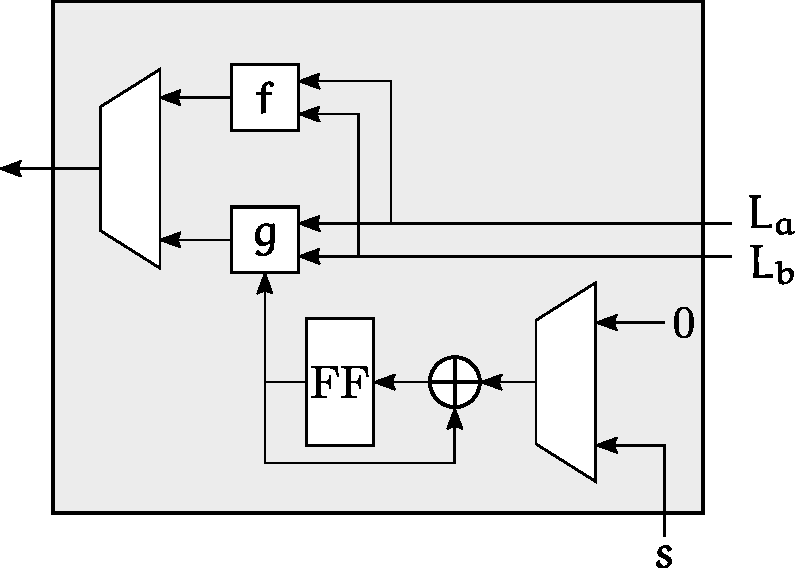
\includegraphics[scale=0.75]{main/ch3_fig/PE}
\caption{Unité matérielle élémentaire (PE : Processing Element).}
\label{fig:pe}
\end{figure}


Les instructions spécialisées choisies pour étendre le jeu d'instructions de l'ASIP s'inspirent des unités de traitement développées dans la littérature pour les circuits dédiés au décodage de codes polaires SC. Dans \cite{leroux_hardware_2011} plusieurs architectures furent proposées. La première architecture proposée est l'architecture \og papillon \fg. Lors du décodage, la fonction $f$ doit être appliqué $N/2$ fois à chaque niveau de l'arbre, et la fonction $g$ également. Au total, il est nécessaire d'appliquer $\frac{N}{2} \log N$ fois les fonctions $f$ et $g$. 

Pour cela, des unités matérielles élémentaires (PE : Processing Elements) sont utilisées.
Un PE permet de réaliser un calcul de $f$ et un calcul de $g$. Un tel élément est représenté dans la figure \ref{fig:pe}.
Dans l'architecture \og papillon \fg, un PE est associé à chaque application des fonctions $f$ et $g$.
Il y a donc au total $\frac{N}{2} \log N$ PEs.
L'application de l'ensemble des fonctions $f$ ou des fonctions $g$ d'un \noeud de l'arbre est alors effectué en un cycle d'exécution.

Cependant, cette architecture est sous-optimale en termes de complexité.
L'ordonnancement de l'algorithme de décodage SC possède les propriétés suivantes :
\begin{itemize}
  \item Le nombre maximum de fonctions polaires élémentaires réalisées simultanément sur un \noeud est $\frac{N}{2}$,
  \item deux \noeuds successifs ne peuvent pas être traités simultanément.
\end{itemize}
En conséquence, les ressources de calculs alloués au traitement d'un \noeud de l'arbre peuvent être utilisé pour le traitements des \noeuds suivants.
Le niveau de parallélisme le plus élevé est $\frac{N}{2}$, donc $\frac{N}{2}$ PEs suffisent pour décoder l'ensemble de l'arbre sans modifier la latence de décodage.
Dans l'architecture \og ligne \fg, $\frac{N}{2}$ PEs sont donc partagées pour le traitement de tous les \noeuds de l'arbre. Sa latence est la même que celle de l'architecture \og papillon \fg.

Dans \cite{leroux_semi-parallel_2013} il est proposé de réduire le nombre de PEs grâce à l'introduction d'une architecture semi-parallèle, de manière similaires à des implémentations précédentes de décodeurs LDPC \cite{1049697}. Dans le décodeur \og ligne \fg, les $\frac{N}{2}$ ne sont toutes utilisées simultanément que deux fois par mot de code décodé. Cela signifie que le taux d'utilisation des PEs est très faible. Il est donc possible de réduire le nombre de PEs sans impacter significativement le débit.
Cette réduction modifie légèrement l'algorithme. En effet les \noeuds nécessitant un nombre d'exécutions de fonctions polaires supérieures à $P$ nécessiteront plus d'un cycle d'horloge à décoder. Le rapport du nombre de PEs d'une architecture semi-parallèle sur le nombre de PEs d'une architecture \og ligne \fg est $N/2P$. Par exemple, pour $N=1024$ et $P=64$, le nombre de PEs est réduit d'un facteur $16$, tandis que le débit est réduit de $2\%$. Pour $N=2^{20}$ et $P=64$, le nombre de PEs est réduit d'un facteur $8192$, et le débit est réduit de moins de $10\%$. L'architecture semi-parallèle s'avère donc très pertinente.

L'architecture proposée dans \cite{sarkis_fast_2014} reprend le principe de l'architecture semi-parallèle. Cependant, les PEs sont modifiés pour intégrer des unités matérielles de traitement des \noeuds spécialisés \texttt{R1}, \texttt{SPC} et \texttt{REP}. Les PEs contiennent également une unité particulière \texttt{REP-SPC} permettant d’accélérer le traitement de deux \noeuds \texttt{REP} et \texttt{SPC} voisins. Ce motif particulier avait été repéré comme apparaissant régulièrement dans le cas traité. Les unités \texttt{REP-SPC} ne sont pas utilisées dans le processeur proposé car ils n'apportent pas de gain significatif pour les tailles de codes considérées ($N<1024$). 

Le dernier type de calcul nécessaire dans l'algorithme de décodage SC est la propagation des sommes partielles (fonction $h$). Dans les implémentations dédiées, les sommes partielles sont sockées dans des registres. Un réseau de portes \textit{ou-exclusif} routées sur ces registres permettent leurs mise à jours instantanées à chaque traitement d'une feuille de l'arbre de décodage. Ce réseau ne fait pas partie des PEs. Dans l'ASIP proposé, les sommes partielles sont stockées dans la mémoire de données, comme les LLRs, afin de les rendre accessibles par le processeur comme toute autre variable. La fonction $h$ fait donc partie des instructions spécialisées conçues pour étendre le jeu d'instructions de l'ASIP proposé.



% Les latences et le nombre de PEs nécessaire pour chaque architecture sont présentées dans le tableau \ref{tab:archis_sc}.

 % \begin{table}[h]
 %    \renewcommand{\arraystretch}{1.1}
 %    \centering
 %    \caption{Latence et nombre de PEs des trois architectures SC.}
 %    \label{tab:archis_sc}
 %    {\small\resizebox{\linewidth}{!}{
 %    \begin{tabular}{l | c  c }
 %    \textbf{Architecture}  & \textbf{Nombre de PEs} & \textbf{Latence (\# cycles)} \\
 %    \cmidrule(lr){1-1}
 %    \cmidrule(lr){2-2}
 %    \cmidrule(lr){3-3}
 %    \og papillon \fg       & $\frac{N}{2} \log N$   & $2N-2$
 %    \og ligne \fg          & $N/2$                  & $2N-2$
 %    \og semi-parallèle \fg & $P$                    & $2N + 
 %    \end{tabular}
 %    }}
 %  \end{table}


\subsection{Instructions spécialisées \textit{multi-registres}}
\label{subsec:multi_reg}

\begin{figure}
\centering
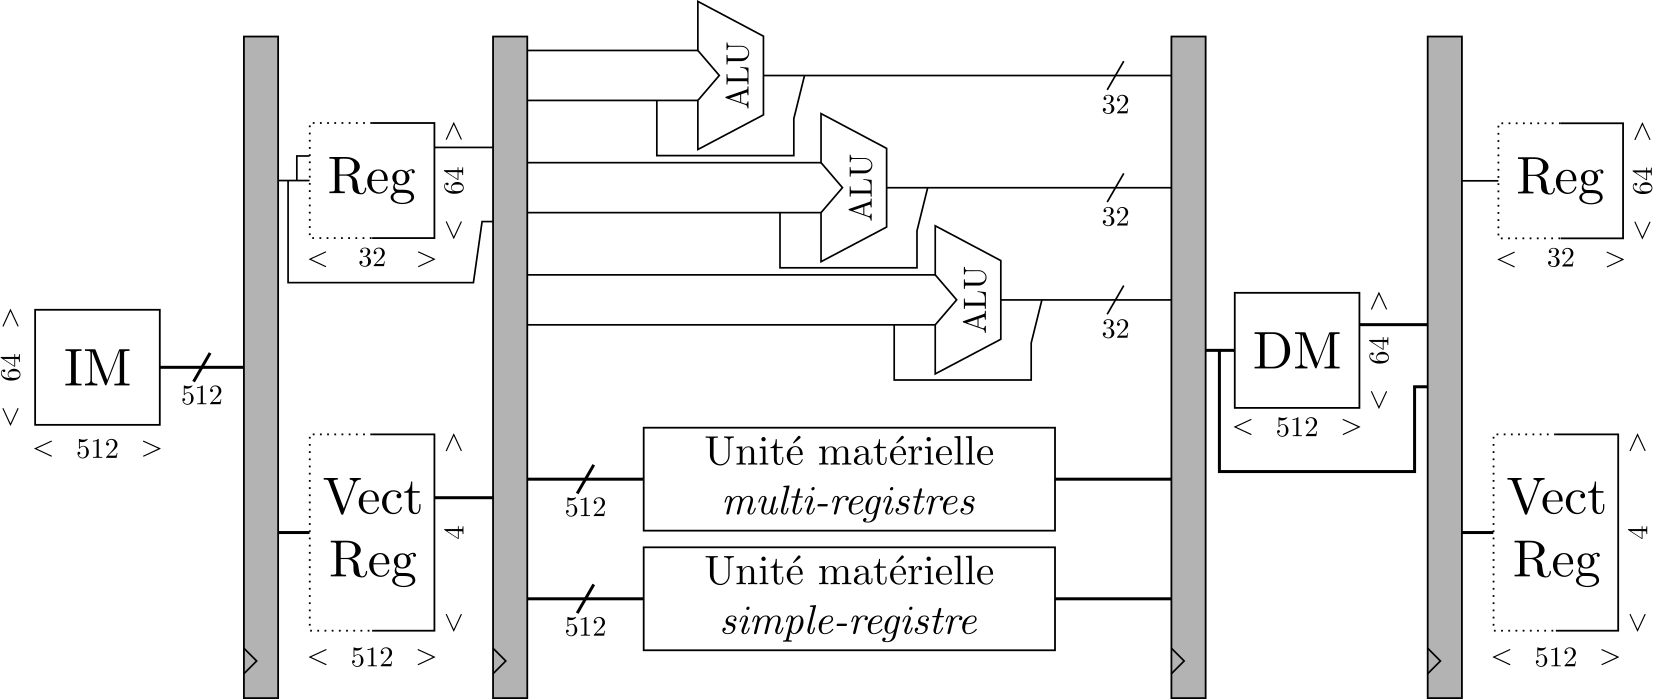
\includegraphics[width=\textwidth]{main/ch3_fig/full_tensilica}
\caption{Architecture de l'ASIP proposé.}
\label{fig:full_tensilica}
\end{figure}

Les instructions spécialisées réalisent des fonctions équivalentes à celles des PEs des architectures matérielles qui ont été présentées dans la sous-section \ref{subsec:hard_sc}. Les fonctions réalisées dans les PEs des architectures que nous venons de présentées sont implémentées dans les instructions spécialisées du processeur proposé : $f$, $g$, \texttt{R1}, \texttt{R0}, \texttt{REP} et \texttt{SPC}. Tout comme dans l'architecture semi-parallèle, le niveau parallélisme $P$ de ces instructions est fixé.

Deux types d'instructions spécialisées ont été conçues et ajoutées au processeur proposé comme montré dans \ref{fig:full_tensilica}. Les premières sont les instructions \textit{multi-registres} et les secondes les instructions \textit{simple-registre}. Leur niveau parallélisme est fixé ($P=64$). Un fichier de registre vectoriel permet de stocker des données de 512 bits. Les instructions \textit{multi-registres} lisent et écrivent dans ce fichier de registre vectoriel.

Ces instructions spécialisées sont donc décrites à l'aide du langage TIE de Tensilica.
L'implémentation de la fonction $f$ est représentée dans la Figure~\ref{fig:f_tie}. Les deux entrées sont les LLRs notés $L_a$ et $L_b$ et la sortie est notée $f(L_a,L_b)$. Ces deux entrées et la sortie correspondent à des registres du fichier de registre vectoriel. Pour rendre claire l'illustration, le niveau parallélisme dans la Figure~\ref{fig:f_tie} a été réduit à $P=4$. Souvent, pour réduire le chemin critique, les LLRs sont représentés en \og signe-amplitude \fg : un bit est utilisé pour le signe, et le reste pour la valeur absolue, toujours positive. Dans notre implémentation, les valeurs négatives sont représentées en complément à deux, car il s'agit du mode de représentation utilisé dans les processeurs XTensa.
La fonction $g$ est représentée dans la Figure~\ref{fig:g_tie}. Elle consiste en une addition simple avec une inversion de signe selon la valeur de la somme partielle $s_a$.
La fonction $h$ n'est pas représentée, il s'agit simplement d'un \textit{ou-exclusif} entre les sommes partielles d'entrées. Les fonctions \texttt{R0} et \texttt{R1} sont également très simples est leur représentation graphique n'est pas utile, puisqu'il s'agit d'une mise à zéro dans le premier cas, et d'un seuillage dans le deuxième, c'est à dire une simple copie du bit de poids fort.
\begin{figure}[t]
  \centering
  \subfloat[Fonction $f$]{
  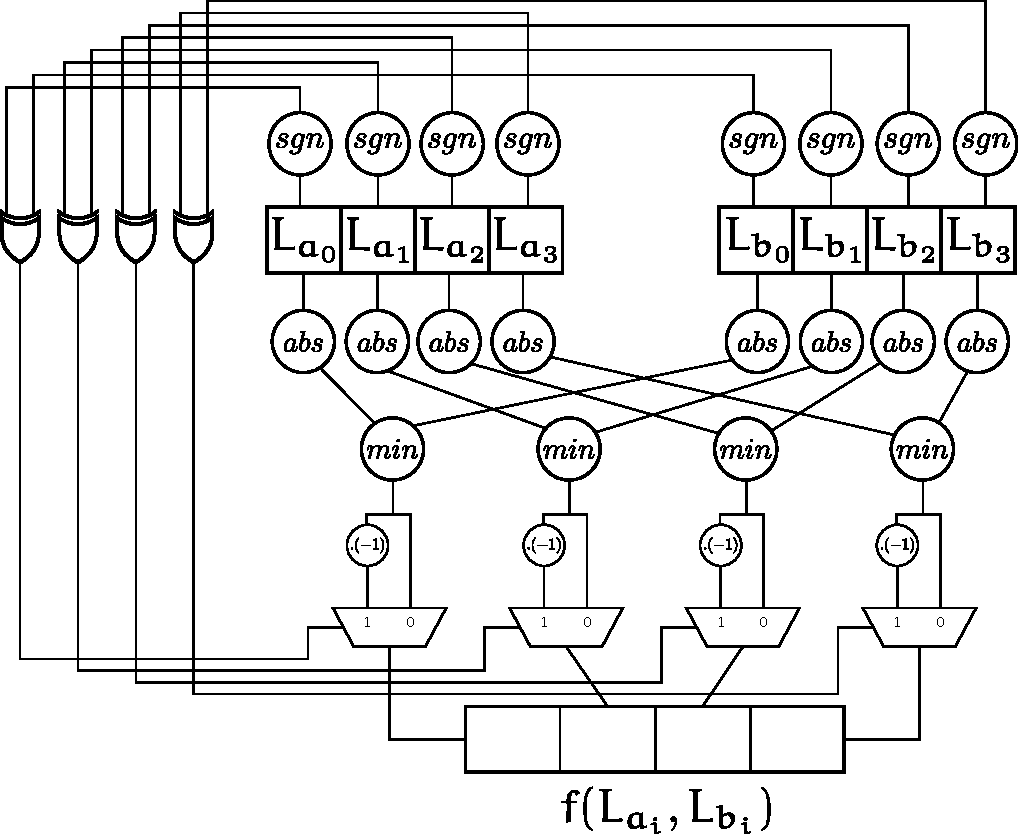
\includegraphics[scale=0.45]{main/ch3_fig/f_tie}
  \label{fig:f_tie}
  }
  \subfloat[Fonction $g$]{
  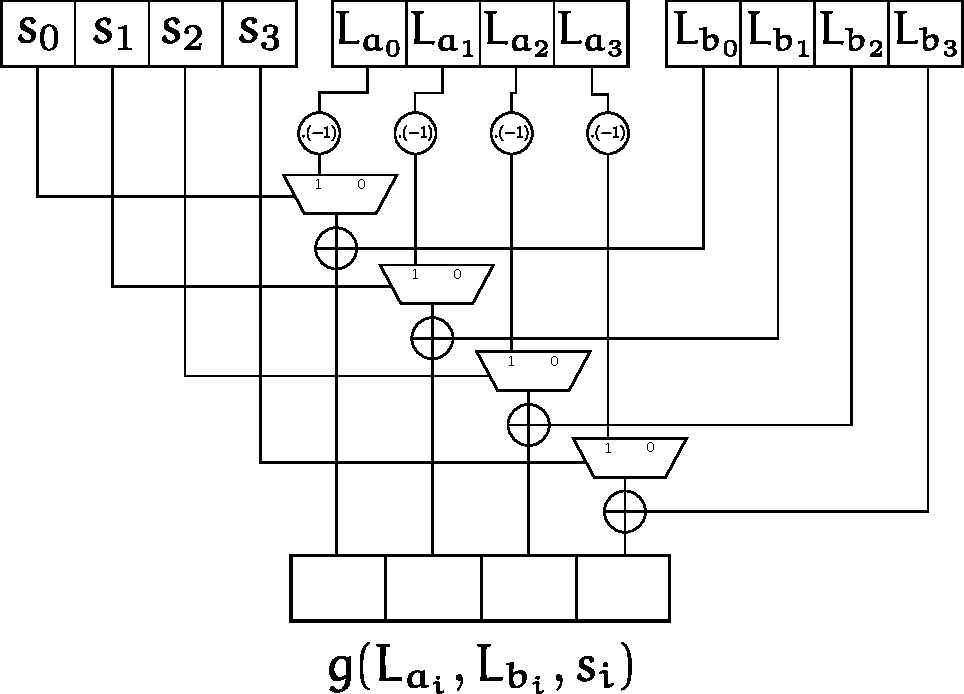
\includegraphics[scale=0.45]{main/ch3_fig/g_tie}
  \label{fig:g_tie}
  }
  \\\quad\quad\quad\quad\quad\quad
  \subfloat[Fonction \texttt{REP}]{
  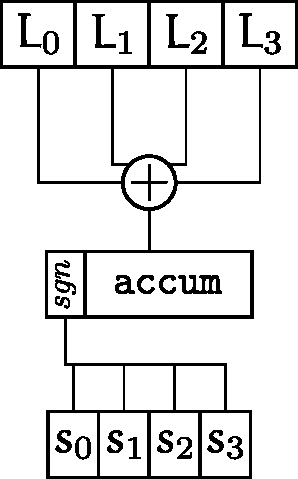
\includegraphics[scale=0.45]{main/ch3_fig/rep_tie}
  \label{fig:rep_tie}
  } \quad\quad\quad\quad\quad\quad\quad\quad\quad\quad
  \subfloat[Fonction \texttt{SPC}]{
  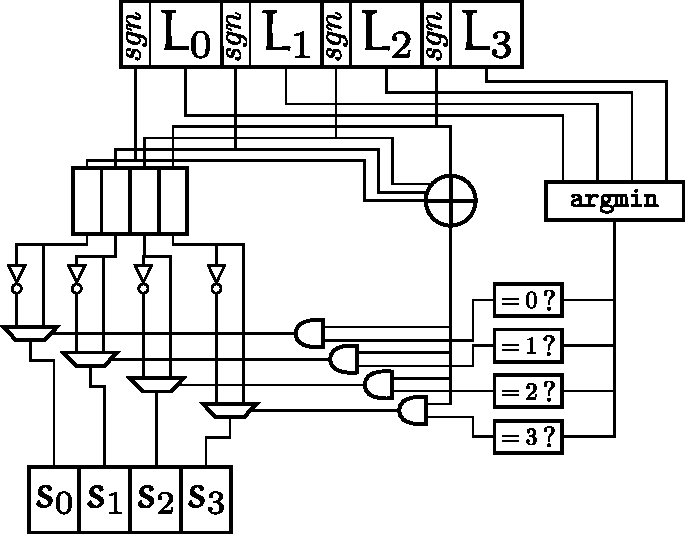
\includegraphics[scale=0.45]{main/ch3_fig/spc_tie}
  \label{fig:spc_tie}
  }
  \caption{Implémentations matérielles des instructions spécialisées.}
\end{figure}

Comme présenté dans la sous-section~\ref{subsec:pruning}, le traitement d'un \noeud de répétition consiste en l'addition de tous les LLRs d'entrée pour former la variable notée \og \texttt{accum} \fg dans la Figure~\ref{fig:rep_tie}. Puis de la détection du signe de cette variable, qui détermine le vecteur $s$ en sortie. Un arbre binaire est parcouru afin de réaliser l'addition nécessaire. Pour éviter tout débordement, la taille du registre de stockage de la variable \texttt{accum} est de 32 bits.

L'unité matérielle de traitement des \noeuds \texttt{SPC} est représentée dans la Figure~\ref{fig:spc_tie}

\subsection{Instructions spécialisées \textit{simple-registre}}

Dans les implémentations logicielles classiques, la séquence d'opérations nécessaire à l'exécution des fonctions élémentaires polaires est la suivante : i) chargement depuis la mémoire cache vers les registres des variables d'entrée (LLRs et / ou sommes partielles), ii) calcul du résultat de la fonction élémentaire, en une ou plusieurs étapes, dont la sortie est stockée dans un registre, iii) sauvegarde de cette variable de sortie dans la mémoire cache du processeur.

\`A l'inverse, dans les implémentations matérielles présentées dans la sous-section \ref{subsec:hard_sc}, le chemin de données part de la sortie de la mémoire, passe par les fonctions combinatoires réalisant les fonctions polaires élémentaires, et finit à l'entrée de la mémoire. Ce chemin de données est parcouru en un seul coup d'horloge. La méthode présentée dans cette sous-section, nommée \textit{simple-registre}, est conçue dans le but de reproduire le fonctionnement des implémentations matérielles de code polaire dans notre processeur.

\begin{figure}[t]
  \centering
  \subfloat[Unité matérielle \textit{simple-registre}.]{
  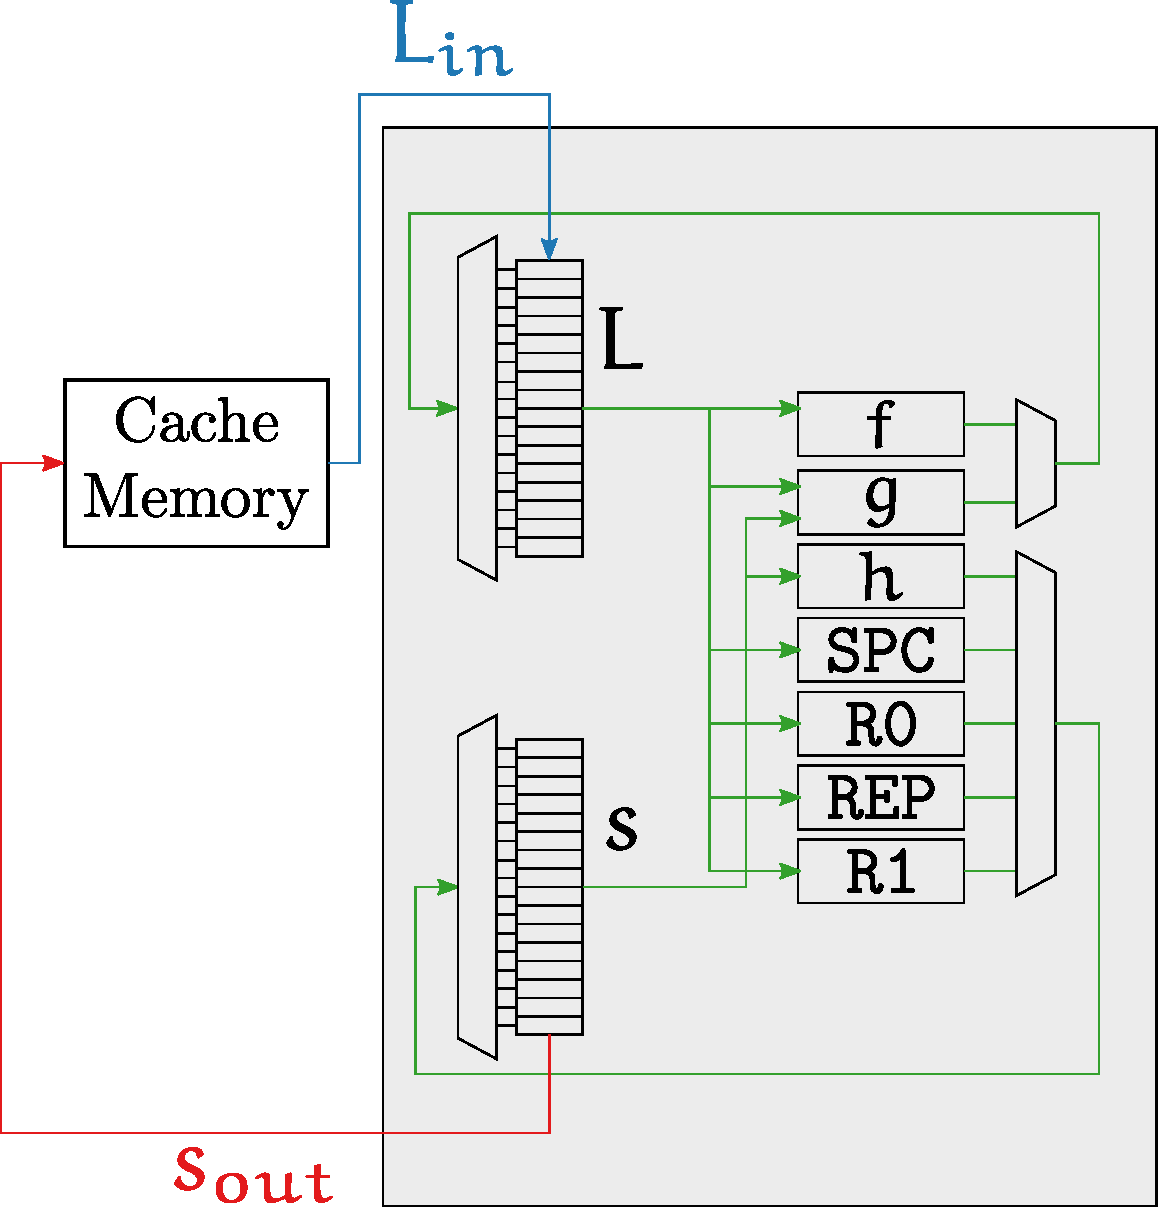
\includegraphics[scale=0.3]{main/ch3_fig/in_register_unit}
  \label{fig:in_register_unit}
  }\quad\quad\quad
  \subfloat[Un sous-arbre décodé grâce aux instructions \textit{simple-registre}.]{
  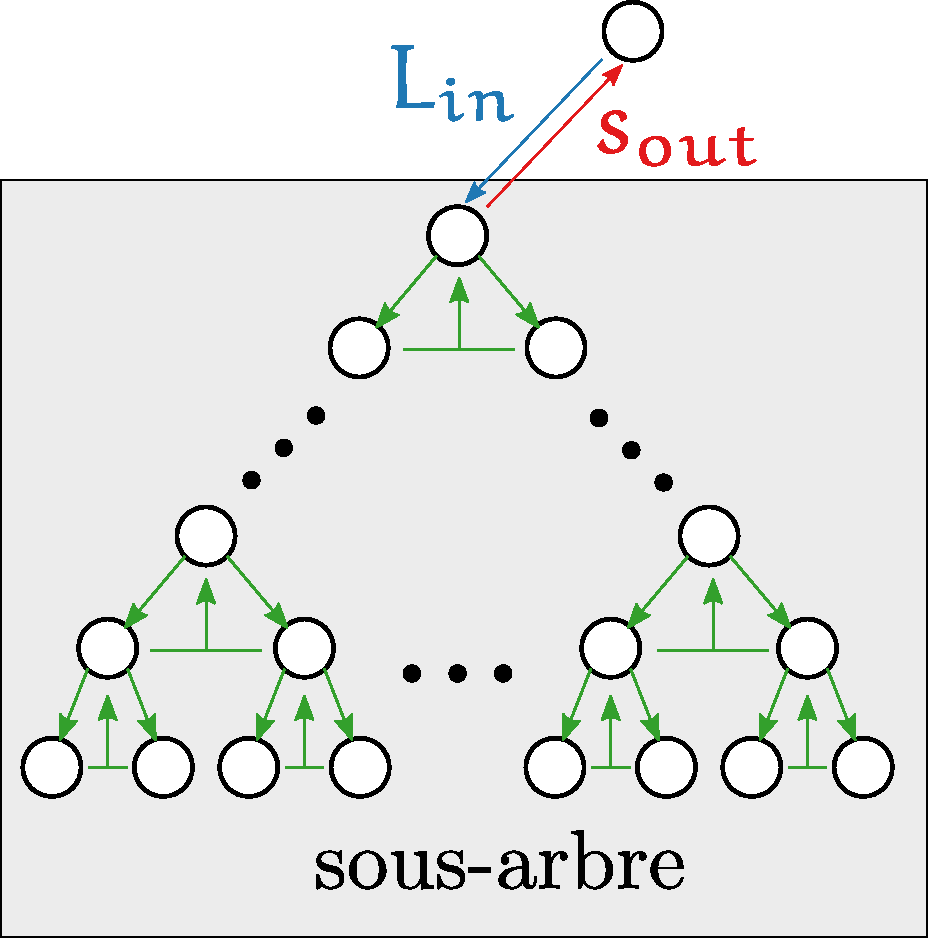
\includegraphics[scale=0.3]{main/ch3_fig/in_register_tree}
  \label{fig:in_register_tree}
  }
  \caption{Instructions \textit{simple-registre}.}
  \label{fig:simple-registre}
\end{figure}

La méthode \textit{simple-registre} est appliquée sur les sous-arbres de décodage dont le \noeud racine contient 64 LLRs. La Figure \ref{fig:in_register_tree} illustre un tel sous-arbre.
Ces 64 LLRs sont notés $\mathbold{L_{in}}$.
Lorsque le programme a généré les LLRs de la racine de ce sous-arbre, ceux-ci sont stockés dans un registre dédié.
Ce registre est noté $\mathbold{L}$ dans la Figure~\ref{in_register_tree} qui représente l'unité matérielle qui réalise les instructions \textit{simple-registre}.
Le décodage du sous-arbre se fait ensuite intégralement dans les registres, sans passer par la mémoire cache.
Les sommes partielles notées $\mathbold{s{out}}$ constituent la sortie de l'unité matérielle.
Cette méthode reproduit le fonctionnement des implémentations matérielles de l'algorithme SC : l'exécution d'une fonction élémentaire quelconque, comprenant la lecture et l'écriture de la donnée depuis le registre, est effectuée en un seul cycle d'horloge.

% \begin{figure}[htp]
% \centering
% 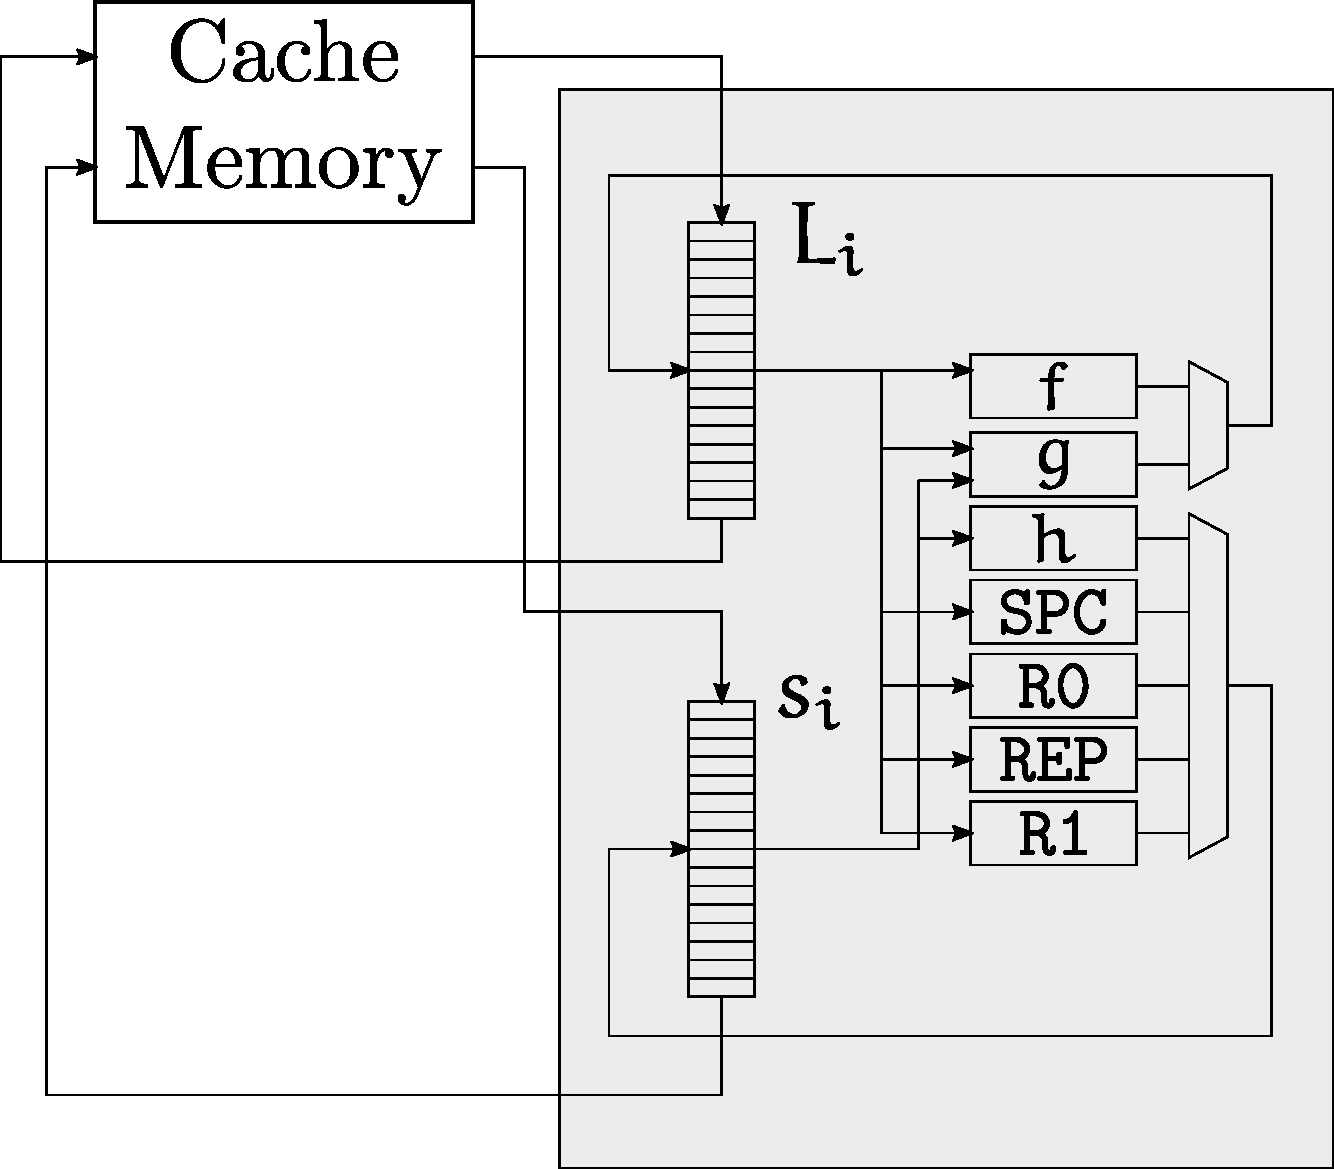
\includegraphics[width=0.7\textwidth]{main/ch3_fig/in_register}
% \caption{Instructions \textit{simple-registre}}
% \label{fig:simple-registre}
% \end{figure}




Elle résout également un problème récurrent des implémentations logicielles utilisant du parallélisme : l'alignement des données. En effet, pour pouvoir appliquer une fonction vectorielle des données de deux registres vectoriels, il est nécessaire de les aligner, ce qui nécessite d'effectuer des opérations supplémentaires. Dans l'implémentation \textit{simple-registre}, l'alignement est prévu en amont et implémenté dans l'unité matérielle. Aucune instruction supplémentaire n'est nécessaire. 

\subsection{Description logicielle}
L'ASIP ainsi proposé permet donc l'exécution efficace de l'algorithme de décodage de codes polaires SC. Le décodage est décrit de manière logicielle, en langage C augmenté des instructions spécialisées. Un extrait du code source est donné dans la Figure~\ref{fig:f_code}. Tout d'abord, les fichiers d'en-tête produits par les outils de conception définissent des types associés aux fichiers de registres vectoriels (\texttt{VR512}). Afin de charger une donnée en mémoire cache vers ces registres vectoriels, il est nécessaire de créer des pointeurs vers ces variables de type (\texttt{VR512}). Les données sont ensuite chargées vers deux de ces registres vectoriels. La fonction spécialisée, ici la fonction \texttt{custom\_f\_64} est ensuite appliquée. Le résultat doit ensuite être stockée dans la mémoire cache.
\begin{figure}[hb]
\lstset{language=C++,
        basicstyle=\footnotesize\ttfamily,
        keywordstyle=\bfseries\color{green!40!black},
        commentstyle=\itshape\color{purple!40!black},
        identifierstyle=\color{blue},
        stringstyle=\color{orange},
        morecomment=[l][\color{magenta}]{\#}
}
\begin{lstlisting}[language=C++, numbers=left, numbersep=0.3em, tabsize=2, basicstyle=\footnotesize\ttfamily]
inline void f_64(signed char* la, 
                 signed char* lb, 
                 signed char* lc)
{
  p512_a = (VR512*) la; // transtyper de char* vers VR512
  p512_b = (VR512*) lb; // transtyper de char* vers VR512
  p512_c = (VR512*) lc; // transtyper de char* vers VR512

  v512_a = *p512_a; // chargement des donnees vers VR512
  v512_b = *p512_b; // chargement des donnees vers VR512
  
  // execution de l'instruction specialisee
  v512_c = custom_f_64(v512_a, v512_b); 
  
  // sauvegarde du resultat en cache
  *p512_c = v512_c;     
}
\end{lstlisting}
\caption{Description logicielle de l'exécution d'une instruction spécialisée.}
\label{fig:f_code}
\end{figure}

Lors du développement, il est apparu qu'il était difficile de réduire le temps passé à réaliser les opérations liées au parcours de l'arbre et aux différents tests. L'utilisation de l'option FLIX3 a permis de réduire ce temps, mais pas suffisamment. La technique de déroulage présentée en sous-section~\ref{subsec:unroll} permet de réduire ce temps. Dérouler le code signifie sacrifier en flexibilité. En effet, il faut générer une version différente du code pour un ensemble donné de paramètres.


\begin{figure}[htp]
\lstset{language=C++,
        basicstyle=\footnotesize\ttfamily,
        keywordstyle=\bfseries\color{green!40!black},
        commentstyle=\itshape\color{purple!40!black},
        identifierstyle=\color{blue},
        stringstyle=\color{orange},
        morecomment=[l][\color{magenta}]{\#}
}
\begin{lstlisting}[language=C++, numbers=left, numbersep=0.3em, tabsize=2, basicstyle=\footnotesize\ttfamily]
// fonction polaire spécialisée
void u_f_64(struct polar_operation& op)
{
    for(int i = 0; i < op.n_elmts; i+=64)
      F_64(op.arg0 + i, op.arg1 + i, op.arg2 + i);
}

// fonction polaire générique
typedef void (*polar_func)(struct polar_operation&);

// structure passée en argument de la fonction générique
struct polar_operation
{
  polar_func   p_func; // pointeur vers la fonction polaire spécialisée 

  signed char* arg0; // les arguments des fonctions polaires spécialisées
  signed char* arg1; // ces arguments sont souvent des adresses
  signed char* arg2;
  signed char* arg3;

  int          n_elmts; // le nombre d'éléments traités en parallèle
  int          off_s; // un offset nécessaire pour l'accès aux PSs
};

// le tableau polar_op_vec est initialisé lors de la construction
// du décodeur il contient la séquence des "polar operation"
std::vector<struct polar_operation> polar_op_vec;

// boucle principale du décodage
virtual void decode()
{
  const int n_op = polar_op_vec.size();
  for (int i = 0; i < n_op; i++)
  {
    // chaque fonction du tableau "polar_op_vec" est appelée
    polar_op_vec[i].p_func(polar_op_vec[i]); 
  }
}
\end{lstlisting}
\caption{Description logicielle du pseudo-déroulage.}
\label{fig:tensilica_code}
\end{figure}
Une alternative est utilisée dans l'implémentation proposée. Tout d'abord, toutes les fonctions élémentaires pour le décodage de code polaires possèdent le même prototype de fonctions dans la description logicielle. Le type de fonction à appliquer ($f$, $g$, $h$, \texttt{R0}, \texttt{R1}, \texttt{SPC}, \texttt{REP}) est passé en paramètre de la fonction, accompagné des adresses auxquelles accéder aux données à lire et écrire. De cette manière, il est possible de créer, un tableau contenant les pointeurs des fonctions à appeler. L'algorithme permettant de déterminer la séquence de fonctions à exécuter prend comme entrée le tableau de bits gelés correspondant au code polaire traité.



\section{Expérimentations et mesures}
\label{sec:tensilica_res}

\subsection{Mesure du gain lié à la spécialisation du processeur.}

Les codes polaires considérés ont été construits selon le document spécifiant les techniques de modulation et de codage pour le standard 5G \cite{3gpp_ts_2017-1}. 
La version académique des outils de design de Tensilica ne permettent pas d'effectuer une synthèse logique du processeur ou d'accéder à sa description RTL. Seules des estimations de la fréquence, de la consommation et de l'aire occupée sont données. Nous avons sélectionné la technologie HPM 28nm de TSMC pour ces estimations.

Le Tableau \ref{tab:evolution_tensilica} présente l'impact des améliorations principales effectuées sur le processeur de base. Un code polaire (32768,29492) est décodé. Les mémoires de données et d'instructions sont dimensionnées pour ce code. La première implémentation logicielle de l'algorithme SC sur l'architecture de base du processeur XTensa LX7 nécessitait 7.3 millions de cycles pour décoder un mot de code. Nous voyons que l'architecture spécialisée pour le décodage de codes polaires combinée à la technique de pseudo déroulage de la description logicielle permet de réduire le nombre de cycles d'un facteur 50. Les instructions \textit{multi-registres} sont responsables d'une grande partie de cette réduction. Elles permettent à elles seules de diminuer d'un ordre de grandeur le nombre de cycles d'exécution.
 \begin{table}[htp]
    \renewcommand{\arraystretch}{1.1}
    \centering
    \caption{Impact de chaque amélioration de l'ASIP sur le nombre de cycles d'horloges nécessaires pour décoder une trame, le débit et la surface occupée. La taille des mémoires n'est pas prise en compte pour la surface occupée. Décodage d'un code polaire (32768,29492). Fréquence considérée : 835 MHz.}
    \label{tab:evolution_tensilica}
    {\small\resizebox{\linewidth}{!}{
    \begin{tabular}{l | c  c  c }
    \multirow{2}{*}{\textbf{Version du processeur}}       & \multirow{2}{*}{\textbf{\# cycles}}   & $\bm{\mathcal{T}_i}$  &   \textbf{Surface}          \\
                                                 &             &  \textbf{(Mb/s)}          &  \textbf{(portes)}          \\
    \cmidrule(lr){1-1}
    \cmidrule(lr){2-2}
    \cmidrule(lr){3-3}
    \cmidrule(lr){4-4}
Processeur de base                               &   $7.30\times10^6$  &   $3.4$            & $160000$             \\

+ instructions \textit{multi-registres} $f$,$g$ et $h$   &   $2.64\times10^6$  &   $9.3$            & $210500$             \\

+ instructions \textit{multi-registres} \texttt{R0},
\texttt{R1},\texttt{SPC} et \texttt{REP}         & $534.00\times10^3$  &   $ 46$            & $272000$             \\

+ FLIX3                                          & $296.00\times10^3$  &   $ 83$            & $311900$             \\

+ instructions \textit{simple-registre}              & $192.00\times10^3$  &   $128$            & $445500$             \\

+ pseudo unrolled                                & $151.00\times10^3$  &   $163$            & $445500$             \\
    \end{tabular}
    }}
  \end{table}


La puissance consommée estimée pour l'ASIP complet est de 111 mW, et l'aire occupée est 0.475 mm\textsuperscript{2}. La fréquence estimée est 835 MHz. Cependant, les instructions spécialisées ne sont pas prises en compte pour l'estimation de la fréquence. En conséquence, un scénario plus pessimiste où la fréquence de fonctionnement est 400 MHz est également présentée. Avec cette fréquence réduite, la consommation estimée devient 49 mW et l'aire occupée 0.374 mm\textsuperscript{2}.

\subsection{Comparaison avec un processeur ARM}

Le logiciel AFF3CT développé par l'équipe CSN du laboratoire IMS de Bordeaux est utilisé pour exécuter une implémentation optimisée de l'algorithme SC sur un processeur ARM Cortex A57. La méthode de parallélisation \textit{intra-trame} est utilisée, et les LLRs sont représentés sur 8 bits avec virgule fixe. La taille des données gérées par les instructions NEON est de 128 bits, donc le parallélisme est égal à 16. Les résultats ici reportés ont été fournis par les auteurs de \cite{cassagne_energy_2016}. Dans ces résultats, la consommation de la mémoire RAM n'est pas prise en compte.
La Figure~\ref{fig:cycle_count} montre le nombre moyens de coups d'horloges nécessaire à chaque processeur pour décoder une trame. Le processeur proposé réduit significativement grâce à l'utilisation d'unités matérielles de calcul spécialisées. La courbe tracée représente le rapport entre les nombres de cycle d'horloge de chaque processeur. Ce rapport est d'autant plus grand que $N$ est faible. Ceci est dû au fait que lorsque $N$ est faible, ce sont les instructions \textit{simple-registre} qui sont le plus utilisées. Or ces instructions sont les plus efficaces.
Cependant, ce nombre réduit de coups d'horloge est contrebalancé par une fréquence réduite comme montré dans le Tableau~\ref{tab:asip}. Néanmoins, même dans le scénario le plus pessimiste, avec une fréquence de 400 MHz, le débit atteint par le processeur proposé est similaire à celui obtenu avec le processeur ARM. Qui plus est, l'énergie dépensée par bit décodé est 10 fois inférieur pour l'ASIP.
\begin{figure}[htp]
\centering
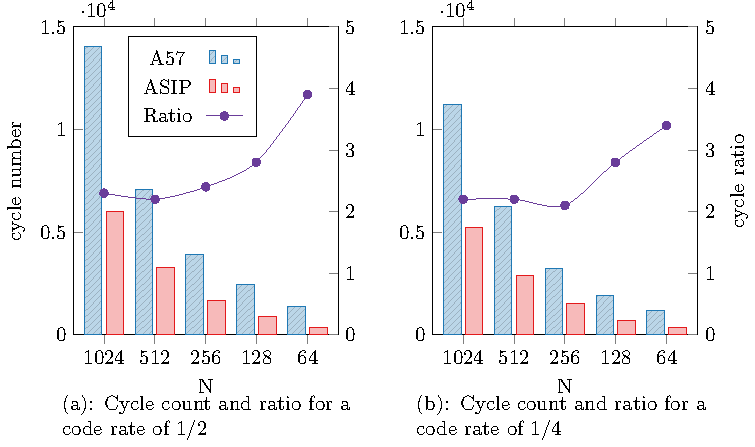
\includegraphics{main/ch3_fig/curves/cycle_count/cycle_count}
\caption{Comparaison du nombre de cycles de l'horloge nécessaires au décodage SC entre le Cortex ARM A57 et l'ASIP proposé.}
\label{fig:cycle_count}
\end{figure}

\subsection{Comparaison avec un processeur d'architecture x86}
Les débits, latences et l'énergie consommée par bit du décodeur logiciel SC inclus dans le logiciel aff3ct ont également été mesurées sur un processeur Intel i7-4712HQ.
La puissance du \coeur est évaluée avec l'outil \texttt{powergadget} d'Intel. Seule la consommation du \coeur du processeur, excluant la consommation de la mémoire cache de niveau 3 et de la mémoire externe, est reportée. Cette fois-ci, le niveau de parallélisme est de 32 grâce à l'utilisation des instructions AVX2. La fréquence du CPU mesurée durant l'exécution est de 3.3 GHz. Les résultats montrent que le débit et la latence des implémentations de décodeur SC sur les processeurs i7 sont bien meilleurs que ceux obtenus avec le processeur ASIP proposé ou avec le processeur ARM. Cependant, la consommation énergétique est moins bonne. Une implémentation \textit{inter-trame} permettrait d'augmenter cette efficacité énergétique, au prix d'une augmentation de la latence, comme démontré dans \cite{cassagne_energy_2016}.


\begin{table}[htp]
  \centering
  \caption{Comparaison de la latence, du débit et de la consommation énergétique de décodeurs SC sur différentes cibles matérielles.}
  \label{tab:asip}
%\scriptsize
  \begin{tabular}{ccccc}
    \toprule

    Target & $N$ & \begin{tabular}{c}Latency\\{[$\mu$s]}\end{tabular} & \begin{tabular}{c}Throughput\\{[Mb/s]}\end{tabular} & \begin{tabular}{c}$E_b$\\{[nJ]}\end{tabular} \\

    \cmidrule(lr){1-1}
    \cmidrule(lr){2-2}
    \cmidrule(lr){3-5}

    \multirow{4}{*}{\bf A57-1.1GHz}
     & $1024$  & $13$  & $38$  & $21$  \\
     & $512$   & $6.7$ & $38$  & $21$  \\
     & $256$   & $3.6$ & $35$  & $22$  \\
     & $128$   & $2.1$ & $30$  & $27$  \\
    \midrule
    \multirow{4}{*}{\bf i7-3.3GHz}
     & $1024$  & $2.3$ & $222$ & $47$  \\
     & $512$   & $1.4$ & $182$ & $57$  \\
     & $256$   & $0.8$ & $155$ & $68$  \\
     & $128$   & $0.5$ & $124$ & $85$  \\
    \midrule
    \multirow{4}{*}{\bf ASIP-835MHz}
     & $1024$  & $7.2$ & $71$  & $1.6$ \\
     & $512$   & $3.9$ & $66$  & $1.7$ \\
     & $256$   & $1.9$ & $65$  & $1.7$ \\
     & $128$   & $1.0$ & $62$  & $1.8$ \\
    \midrule
    \multirow{4}{*}{\bf ASIP-400MHz}
     & $1024$  & $15$ &  $34$  & $1.4$ \\
     & $512$   & $8.2$ & $31$  & $1.6$ \\
     & $256$   & $4.1$ & $31$  & $1.6$ \\
     & $128$   & $2.1$ & $30$  & $1.7$ \\
    \bottomrule
  \end{tabular}
\end{table}

\section*{Conclusion}

La première architecture de processeur ASIP spécialisé dans le décodage de codes polaires est présentée dans ce chapitre. Les outils logiciels Tensilica permettent de particulariser un processeur de type RISC. Après avoir détaillé la structure générales de ces microarchitectures RISC, nous expliquons comment elles peuvent être configurées et étendues par l'utilisation des outils logiciels Tensilica. Les avantages et les enjeux liés à l'utilisation de tels outils de conception sont mis en avant.

Dans la seconde partie du chapitre, nous expliquons comment ces outils ont été mis en œuvre pour notre problématique : le décodage de codes polaires. Tout d'abord les paramètres de l'architecture RISC de base sont modifiés et adaptés. Entre autres, une fonctionnalité permettant le support d'un parallélisme d'instruction est activée, et la largeur du bus d'interface avec la mémoire de données est augmentée. Ensuite, des unités matérielles dédiées associées à des instructions spécialisées qui étendent le jeu d'instructions de base sont ajoutées. Enfin, une méthode de description logicielle nommée \og pseudo-déroulage \fg est proposé afin d'améliorer les performances de débit et de latence du processeur spécialisé conçu.

Dans une troisième partie, nous présentons et comparons le débit, la latence et la consommation du décodeur proposé avec les implémentations logicielles de codes polaires de l'état de l'art. Pour un code polaire (1024,512) décodé à l'aide de l'algorithme SC, le débit atteint est d'environ 70 Mb/s, dépassant les performances obtenues avec un processeur du marché de l'électronique embarquée. La consommation énergétique par rapport à ce même processeur est elle réduite d'un ordre de grandeur.

Bien que ces résultats soient prometteurs, plusieurs limites concernant l'utilisation des outils et de la méthodologie Tensilica ont été identifiées. Tout d'abord, le défaut d'une licence complète empêche la génération du modèle matériel du processeur. Il est donc impossible de générer des résultats complets de synthèse et d'implémentation. Pour cette raison, les résultats obtenus sont des estimations fournies par l'outil, avec une marge d'erreur importante. Ensuite, le langage de descriptions matériel est le langage TIE, spécifique à la suite logicielle Tensilica. Ceci réduit la réutilisabilité des unités matérielles conçues. D'autre part, une analyse attentive du code assembleur généré et des résultats de simulations montrent qu'une part très importante de la durée d'exécution est prise par les échanges de données entre la mémoire cache, les registres et les unités matérielles de calcul. La conception et l'ajout des instructions \textit{simple-registre} sont permettent de diminuer le nombre de ces échanges. Mais cette amélioration est partielle et ne peut pas être utilisée sur l'ensemble de l'arbre de décodage.

Plusieurs outils de conception d'ASIP ont été envisagés afin de résoudre ces problèmes. Parmi eux, la famille d'architectures \og TTA \fg a été sélectionnée pour créer le processeur présenté dans le chapitre suivant. Une des raisons de ce choix est la possibilité de bypasser les registres et d'échanger les données directement entre la mémoire de données et les unités matérielles.             % Troisième thème (Doctorat) ou effacez ce fichier si vous êtes à la Maîtrise.
%!TEX root = ../my_thesis.tex
\chapter{Décodeurs polaires déclenchés par transport} % (fold)
\label{chap:tta}

\vspace*{\fill}
\minitocTITI
\vspace*{\fill}
\newpage

\section*{Introduction}



\section{Transport Triggered Architectures}


\subsection{Principes}

Au cours de ce manuscrit, du point de vue de l'architecture des processeurs, deux types de parallélisme ont été abordés.
Le premier est le parallélisme de données.
Pour exploiter ce parallélisme, les jeux d'instructions de certains processeurs incluent des instructions vectorielles SIMD.
C'est le cas des architectures ARM ou x86 actuelles qui incluent respectivement les jeux d'instructions NEON et AVX utilisés dans le Chapitre \ref{chap:soft_scl}.
Les instructions spécialisées de l'ASIP proposé dans le Chapitre \ref{chap:tensilica} sont également des instructions SIMD.
Ces instructions permettent d'appliquer parallèlement une même opération sur plusieurs données.

Le second type de parallélisme est le parallélisme d'instructions. Contrairement au parallélisme de données, il s'agit d'exécuter plusieurs opérations différentes sur plusieurs données d'entrées. Par exemple, effectuer une somme de deux données et, en parallèle, effectuer une opération \textit{ou-exclusif} sur deux autres.
Il existe plusieurs façons de concevoir un processeur permettant du parallélisme d'instructions. Le compilateur peut selon les cas être impliqué dans la détection et l'exploitation du parallélisme d'instructions.

Dans les architecture superscalaires, le compilateur n'est pas impliqué dans la gestion du parallélisme d'instructions. Celui-ci est détecté par des unités matérielles spécialisées. 
Elles permettent de lancer l'exécution de plusieurs opérations parallèles sur les multiples unités fonctionnelles du processeur.
Pour cela, ces unités ont la capacité d'analyser les dépendances entre les données, de changer dynamiquement l'ordre d'exécution des instructions, ainsi que de spéculer sur les futures instructions du programme exécuté. 
Un des avantages de ce type de processeurs est que des programmes séquentiels d'architectures plus anciennes peuvent être accélérés sans nouvelle compilation. Le désavantage est le complexité accrue du processeur causée par l'ajout des unités matérielles responsables de la mise en œuvre du parallélisme. La surface du circuit augmente, ainsi que sa consommation énergétique \cite{rau1993instruction}.

Au contraire, dans les architectures dites \og à très long mot d'instruction \fg (VLIW : Very Large Instruction Word), l'essentiel de l'effort nécessaire à la mise en œuvre du parallélisme d'instructions est pris en charge par le compilateur. Le compilateur décrit quelles instructions doivent être exécutées en parallèle, et dans quel ordre. L'avantage des architectures VLIW par rapport aux architectures superscalaires est la réduction de la complexité de la logique de contrôle. De plus, les possibilité de parallélisme d'instructions sont plus facilement identifiées par les compilateurs qui ont une vue plus large du programme que les unités matérielles de parallélisation des architectures superscalaires.


\begin{figure}[htp]
\centering
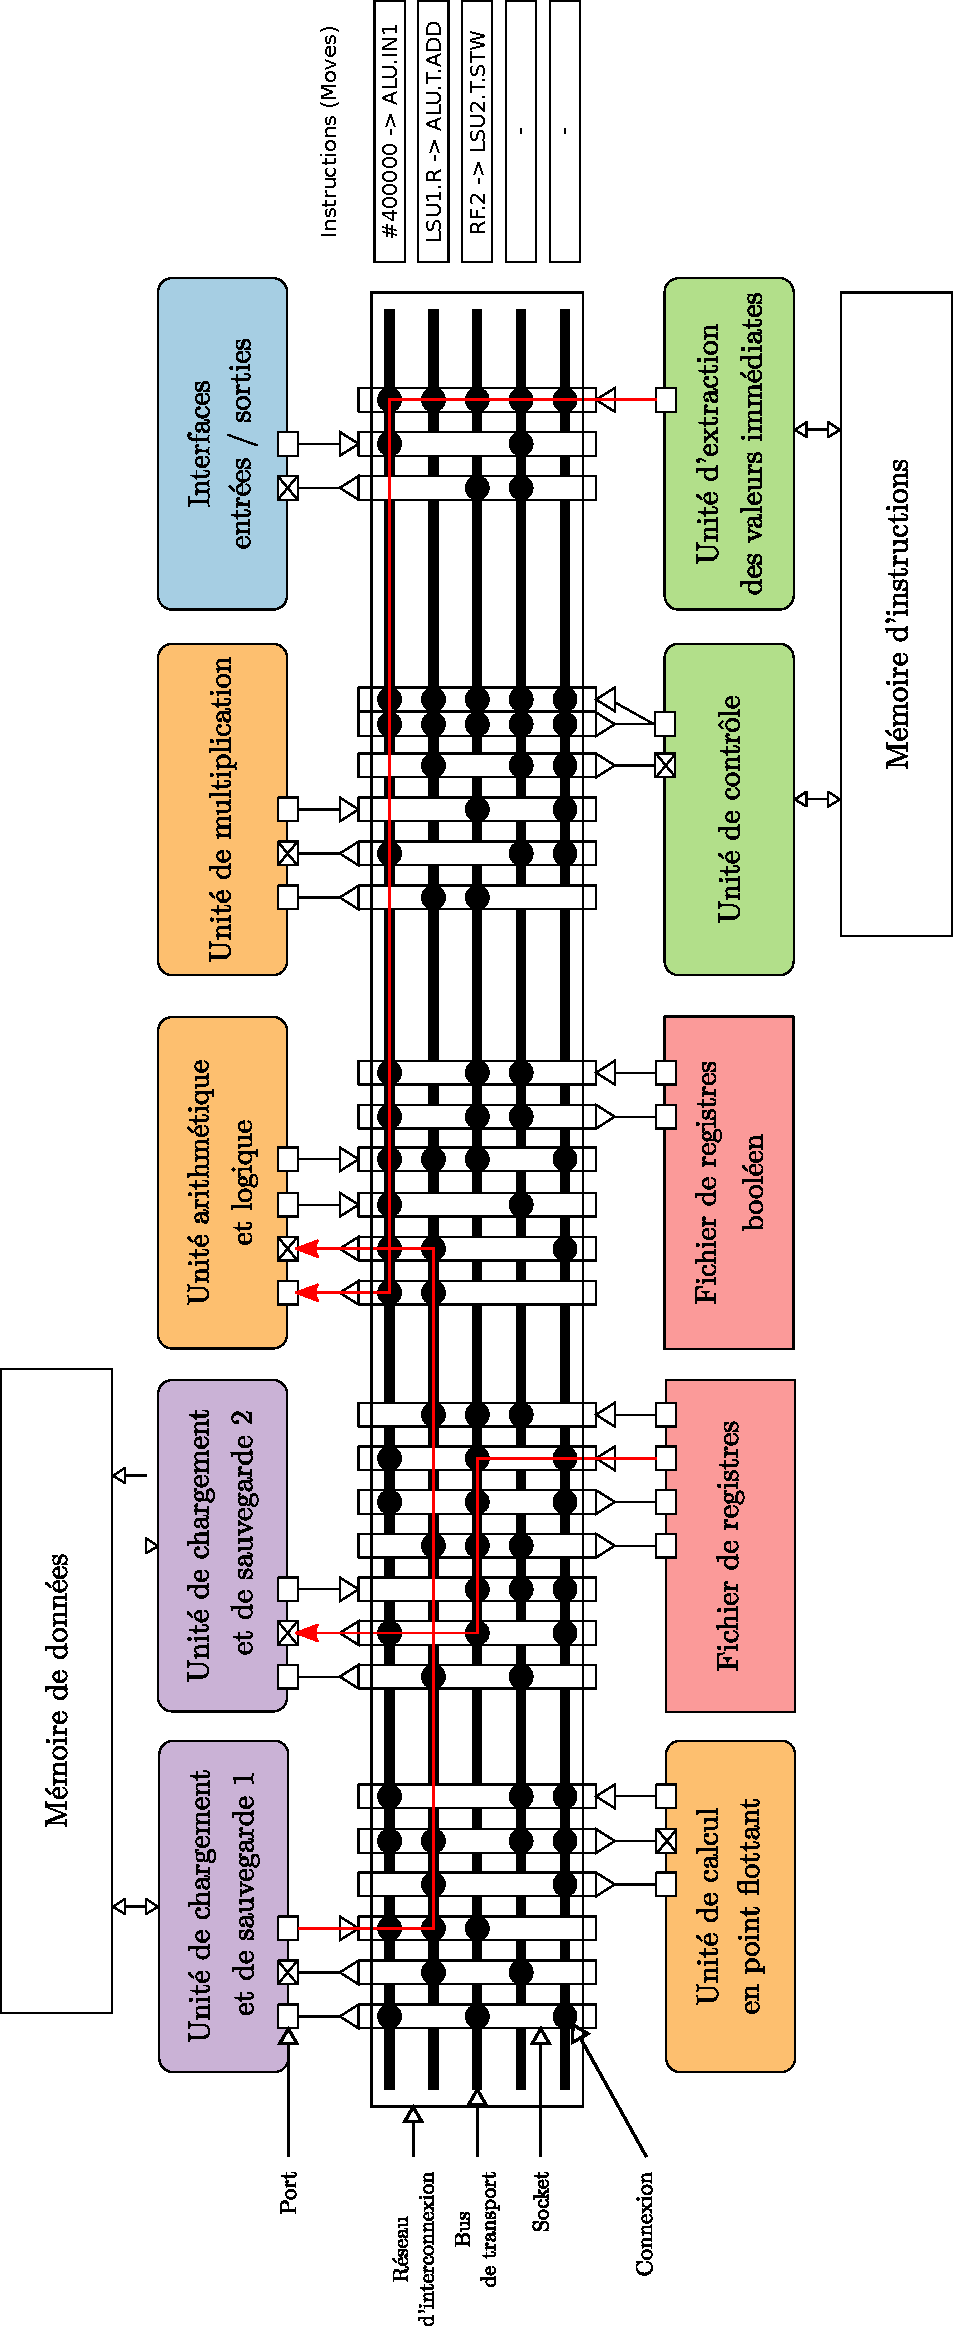
\includegraphics[width=\textwidth]{main/ch4_fig/archi_tta}
\caption{Un exemple d'architecture de processeur TTA.}
\label{fig:tta_example}
\end{figure}

L'architecture de processeur proposée dans ce chapitre fait partie de la famille des architectures déclenchées par le transport (TTA : Transport Triggered Architecture). Les TTAs sont des architectures modulaires particulières proches des architectures VLIW \cite{corporaal_microprocessor_1997}. Les TTAs sont inspirées des architectures MOVE \cite{1051344}. La Figure \ref{fig:tta_example} présente un exemple d'architecture TTA \cite{pekka_phd_2012}. Au centre, on trouve les \textit{bus de transport} sur lesquels les données transitent. Sur ces bus de transport sont connectées les \textit{unités fonctionnelles}, par l'intermédiaire des \textit{socket} et des \textit{ports}. Les \textit{ports} font partie des \textit{unités fonctionnelles} : ils en constituent l'interface avec le monde extérieur. Une \textit{socket} est associée à chaque port. Elle n'est pas forcément connectée à tous les bus de transport. Lors de la définition du processeur, c'est le rôle du concepteur de décider quels \textit{bus de transport} doivent être connectés à une \textit{socket}. Le nombre de \textit{connexions} doit être maitrisé afin de limiter la complexité du \textit{réseau d'interconnexion}.

La différence principale séparant les architectures VLIW classiques et les architectures TTA sont les instructions utilisées. Dans les architectures VLIW, les instructions correspondent aux opérations à effectuer à chaque cycle d'instructions. Des registres d'entrée et de sortie peuvent y être spécifiés, selon le type d'instruction. En revanche, un programme exécuté par un processeur d'architecture TTA contient une séquence de transports de données, depuis un port d'une unité fonctionnelle vers un autre. Les opérations sont exécutées lorsqu'une donnée est transportée vers un port particulier d'une unité fonctionnelle, nommé \textit{port de déclenchement}. Chaque unité fonctionnelle possède un seul port de déclenchement. Ces ports sont représentés dans la Figure \ref{fig:tta_example} sous la forme d'une croix inscrite dans le carré du port.

Dans l'exemple, trois transports sont effectués sur les trois bus de gauche, tandis que les deux bus de droite sont inutilisés. Les instructions correspondantes sont représentées au dessus du réseau d'interconnexion. Le langage utilisé pour définir les transports est le langage assembleur des architectures TTA, proche du contenu du programme compilé. Sont définis deux ports, le premier est la source, le second la destination. Le port est lui-même spécifié par le nom de son unité fonctionnelle et un identifiant. Lorsque le port de sortie est un port de Déclenchement (T : Trigger), l'opération déclenchée est également spécifiée. Par exemple, le deuxième transport a pour cible le port de déclenchement de l'unité arithmétique et logique (ALU : Arithmetical and Logical Unit). Il est précisé alors que l'opération d'addition (ADD) doit être déclenchée (ALU.T.ADD).

Augmenter le nombre d'unités fonctionnelles d'une architecture VLIW est problématique car il est nécessaire d'augmenter le nombre de ports d'écritures et de lecture des fichiers de registres afin de que les unités fonctionnelles puissent y accéder simultanément. Ceci a pour conséquence une augmentation de la complexité des fichiers de registre et une possible augmentation du chemin critique.
La modularité des architectures TTA résoud ce problème.

En effet, le réseau d'interconnexion et les chemins de données disponibles sont connus du programmeur et du compilateur. On parle de \og chemin de données exposé \fg (\textit{exposed datapath}). Comme le programmeur définit la séquence des transports, et non la séquence des opérations à exécuter, il n'est pas nécessaire de dimensionner les ports des fichiers de registre par rapport au pire cas du nombre d'unités fonctionnelles pouvant accéder simultanément à un fichier de registres. Le programmeur ne peut qu'affecter des transports de données à des bus libres.

De plus, dans les architectures VLIW, les mécanismes de dérivation des registres (\textit{register bypass}) sont implémentés matériellement. Dans les architectures TTA, ils sont décrits par le programmeur logiciellement. Cela permet de réduire encore davantage l'engorgement des registres et donc la nécessité de ports supplémentaires sur chaque fichier de registres.

Ce sont ces différents avantages qui ont guidé notre choix dans la sélection des architectures TTA pour la conception d'architectures programmables de décodage de codes polaires. Elles résolvent en effet le problème identifié en conclusion du chapitre \ref{chap:tensilica} du nombre d'échanges nécessaires entre les mémoires, les fichiers de registres et les unités fonctionnelles. La modularité des architectures TTA nous permet de définir finement un réseau d'interconnexion permettant des communications directes entre les mémoires et les unités fonctionnelles, mais également entre les unités fonctionnelles elle-même.

Une autre raison de ce choix est l'existence d'une suite logicielle libre nommée TCE permettant un conception efficace d'architectures TTA. Elle offre également un compilateur adaptatif qui permet l'écriture de programme dans des langages de haut niveau (C / C++). Cette suite logicielle est décrite dans la sous-section suivante.


\subsection{Environnement TCE}

\subsubsection{Définition de l'architecture et de l'implémentation du processeur}

L'environnement TCE (TTA-based Co-design Environment) est une suite d'outils logiciels permettant la description d'architectures TTA, la compilation de programmes exécutables sur ces architectures, et la génération de modèles matériels synthétisables et implémentables \cite{jaaskelainen_hw/sw_2017}. Une version améliorée de l'outil, nommée TCEMC (TCE MultiCore), permet le support d'opérations SIMD \cite{tcemc_2011}. Elle est utilisée pour concevoir les décodeurs polaires proposés. La Figure \ref{fig:tce} présente l'ensemble des outils proposés, les fichiers intermédiaires produits et utilisés et le flot de conception.

Le premier outil utilisé est l'éditeur de modèle architectural (\textbf{prode}). Il s'agit d'une interface graphique. Il permet de définir une architecture TTA telle que celle illustrée dans la figure \ref{fig:tta_example}. Le fichier \textit{.adf} contient le nombre de bus et la largeur de chaque bus, la liste des sockets et de leurs connexions avec les bus de transport et les ports des unités fonctionnelles. Il contient aussi la liste des unités fonctionnelles.

Il contient également les opérations que chaque unité fonctionnelle est capable de réaliser. Chaque opération est décrite par son interface, contenue dans un fichier \textit{.opp} et son comportement, défini par un fichier \textit{.c} ou \textit{.cpp}. L'éditeur de la base de données des opérations (\textbf{osed}) permet d'explorer et d'éditer les différentes opérations. Il permet également de compiler les modèles comportementaux. L'exécutable (\textit{.opb}) permet d'effectuer des simulations de l'opération, soit de manière individuelle, soit au sein du simulateur du programme complet. L'outil \textit{prode} associe les unités fonctionnelles avec les opérations dans le fichier \textit{.adf}.

\begin{figure}[htp]
\centering
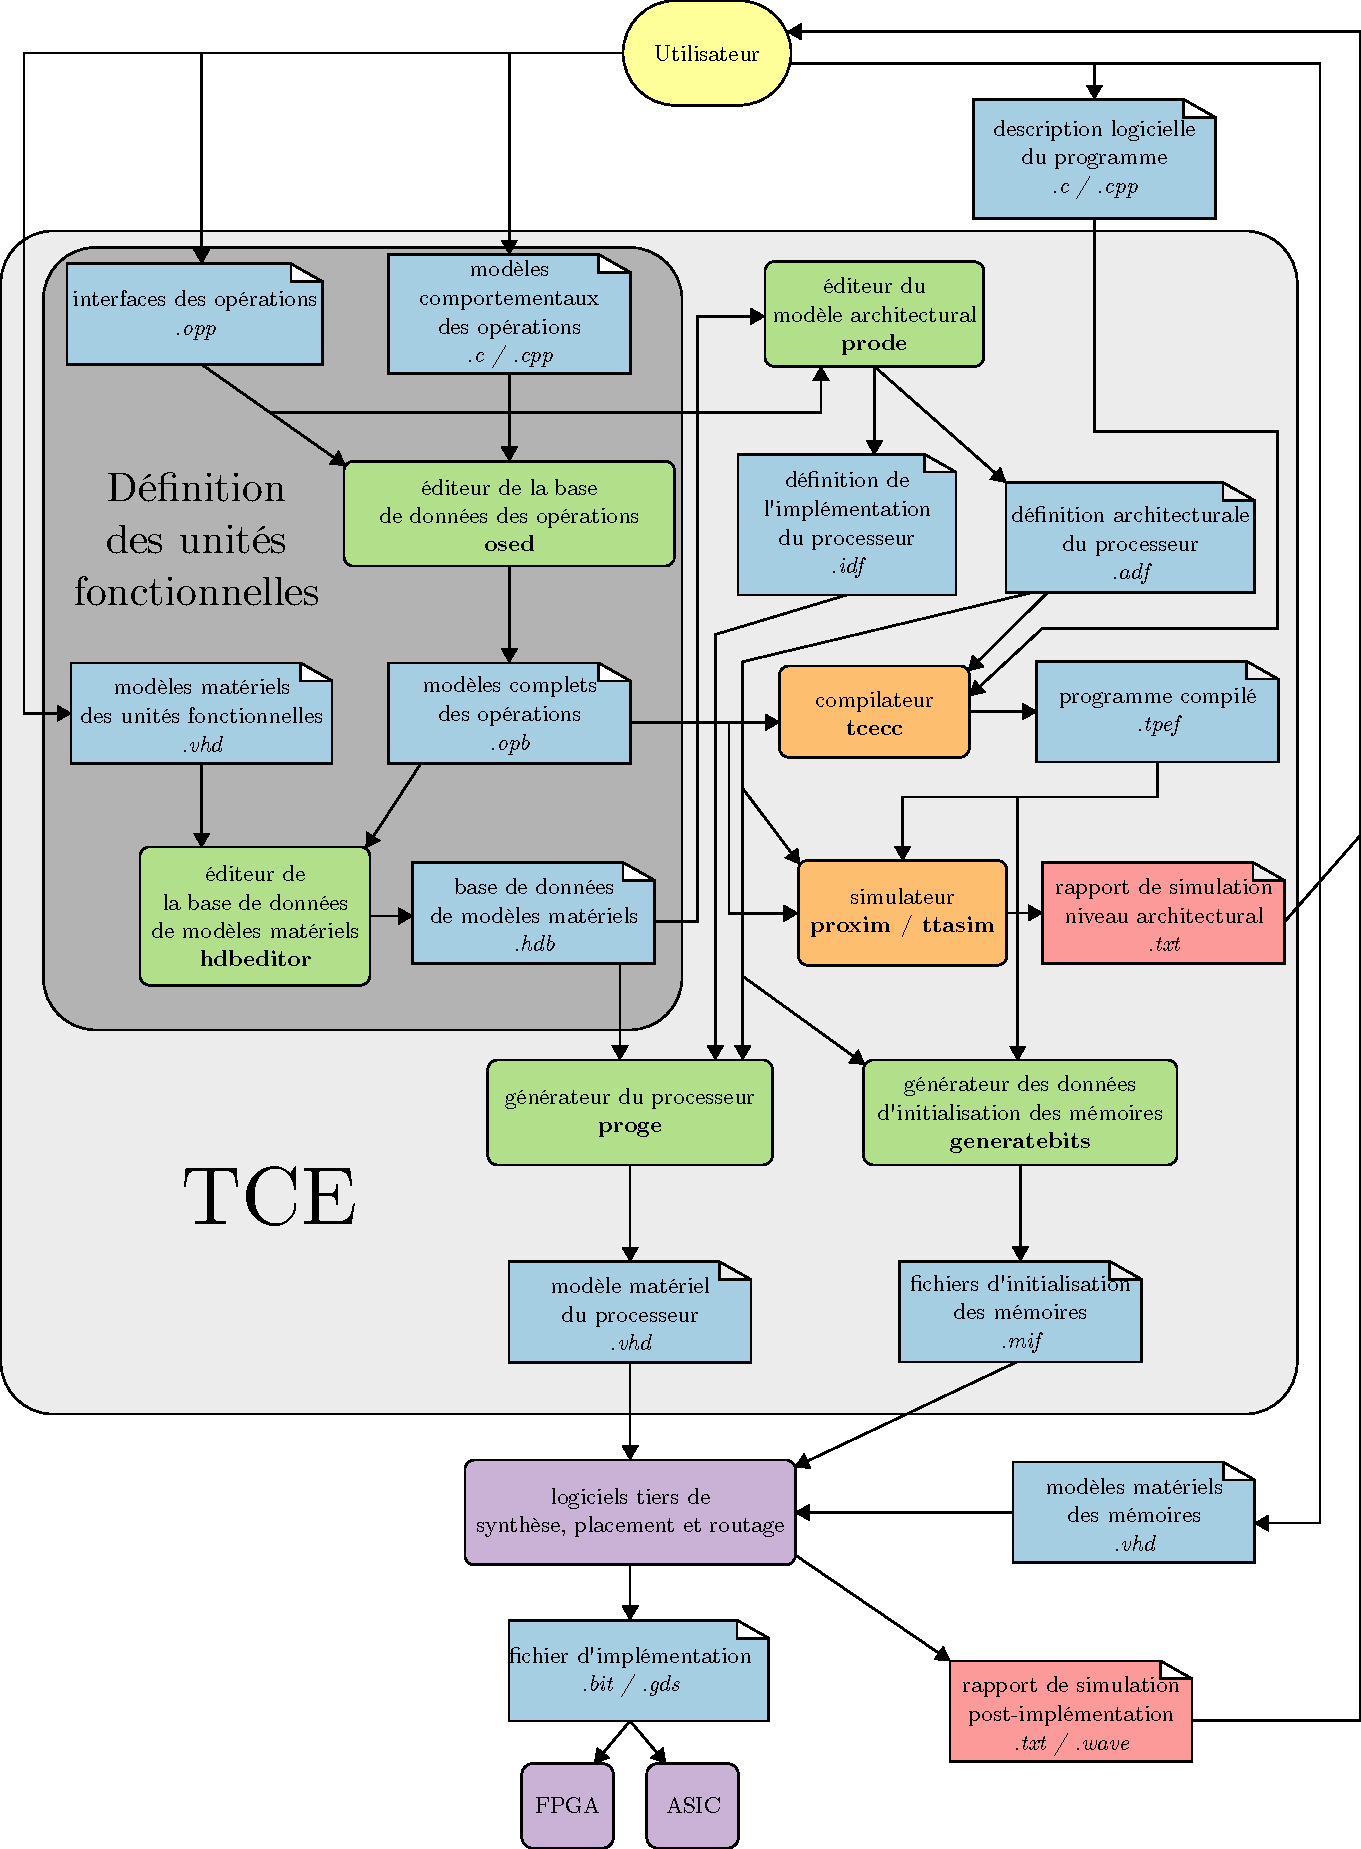
\includegraphics[width=\textwidth]{main/ch4_fig/tce}
\caption{Le flot de conception TCE.}
\label{fig:tce}
\end{figure}
Les modèles matériels des unités fonctionnelles sont décrits en langage VHDL ou Verilog. Un grand nombre de modèles matériels et d'opérations de base sont fournies par la suite logicielle TCE (unités de chargement et de sauvegarde, fichiers de registres, ALU, unités SIMD, ...). Pour créer des unités fonctionnelles spécifiques, l'utilisateur doit décrire l'interface des opérations, leurs modèles comportementaux, et les modèles matériels des unités fonctionnelles dans un langage de description matériel (VHDL ou Verilog). Ces modèles matériels sont réunis dans une base de données de modèles matériels (\textit{.hdb}), éditable et consultable grâce à l'outil \textit{hdbeditor}.
La base de donnée sert au concepteur afin de réutiliser des modèles matériels déjà conçus par lui même ou par d'autres contributeurs.

Le deuxième fichier produit par \textbf{prode} est le fichier de définition de l'implémentation \textit{.idf}. Il relie simplement chaque unité fonctionnelle définie dans le fichier \textit{.adf} à son implémentation matérielle contenue dans la base de donnée de modèles matériels.

\subsubsection{Simulation au niveau architectural.}

Le compilateur (\textbf{tcecc}) utilise le fichier de description architecturale \textit{.adf} et les modèles des opérations afin de compiler la description logicielle du programme écrite par le programmeur. Ce programme est écrit dans un langage haut niveau (C,C++,OpenCL). Un effort particulier a été effectué par les développeurs de l'environnement TCE afin de rendre ce compilateur efficace. Il est basé sur le projet LLVM \cite{lattner_llvm:_2004} et bénéficie à ce titre d'optimisations des premiers niveaux de la chaîne de compilation (analyses lexicale, syntaxique, sémantique et génération du code intermédiaire). Les dernières étapes d'optimisation spécifiques a TTA (dérivation des fichiers de registre, utilisation d'unités fonctionnelles, opérations SIMD) sont réalisées par les développeurs de l'outil TCE.

Le programme compilé peut ensuite être simulé, soit à l'aide d'un outil en ligne de commandes (\textbf{ttasim}), soit par une interface graphique (\textbf{proxim}). Cette simulation permet d'obtenir le nombre de cycles nécessaire à l'exécution de l'intégralité ou d'une partie du programme, et ainsi d'avoir un premier retour sur l'efficacité de l'architecture conçue. D'autres fonctions sont accessibles grâce à ce simulateur. Un profilage peut être réalisé. Il permettra à l'utilisateur de connaître le nombre de cycles d'exécutions pris par chaque fonction et ainsi de connaître les portions du programmes à accélérer prioritairement. Le simulateur donne également des métriques importantes, comme l'engorgement des bus, l'engorgement des sockets ou le taux d'utilisation de chaque opération dans les unités fonctionnelles. Cet ensemble de métriques permet au concepteur d'analyser très finement le fonctionnement du processeur et le déroulement du programme.

\subsubsection{Génération du processeur.}

La dernière étape est la génération du modèle matériel complet du processeur. L'outil de génération du processeur (\textbf{proge}) utilise la base de données des modèles matériels des unités fonctionnelles (fichier \textit{.hdb}) ainsi que les fichiers de description de l'architecture et de l'implémentation du processeur (fichiers \textit{.adf} et \textit{.idf}) afin de créer le modèle complet du processeur. Il intègre donc les différents modèles des unités fonctionnelles, le réseau d'interconnexion, mais également l'unité de contrôle du processeur, visible dans la Figure \ref{fig:tta_example}, qui permet la lecture du programme, stocké dans la mémoire d'instructions.

L'outil \textbf{generatebits} permet quant à lui de générer les contenus d'initialisation des mémoires de données et d'instructions. Les modèles matériels de ces mémoires doivent être fournis par l'utilisateur puiqu'en général, ceux-ci sont dépendants de la cible d'implémentation.

Le modèle matériel du processeur, décrit dans un langage de description matériel (VHDL ou Verilog) et les modèles des mémoires peuvent ensuite être fournis à un logiciel tiers, pour synthèse et implémentation sur FPGA ou sur ASIC. Les rapports de synthèse ou d'implémentation fournissent alors des métriques concernant la fréquence de fonctionnement, la surface utilisée et la consommation de puissance. Ces métriques peuvent être utilisées par le concepteur afin d'améliorer l'architecture du processeur. Des itérations du flot de conception permettent d'améliorer le processeur jusqu'à l'obtention de performances satisfaisantes.



\section{Transport Triggered Polar Decoders}
Deux architectures de processeurs spécialisés dans le décodage de codes polaires ont été conçues et seront présentées dans cette section. La première est spécialisée dans le décodage SC, elle est nommée \TTSC. La seconde supporte le décodage efficace de l'algorithme SC et de l'algorithme SCAN, elle est nommée \TTSCAN

\subsection{Architecture du décodeur \TTSC}

\begin{figure*}[t]
	\centering
	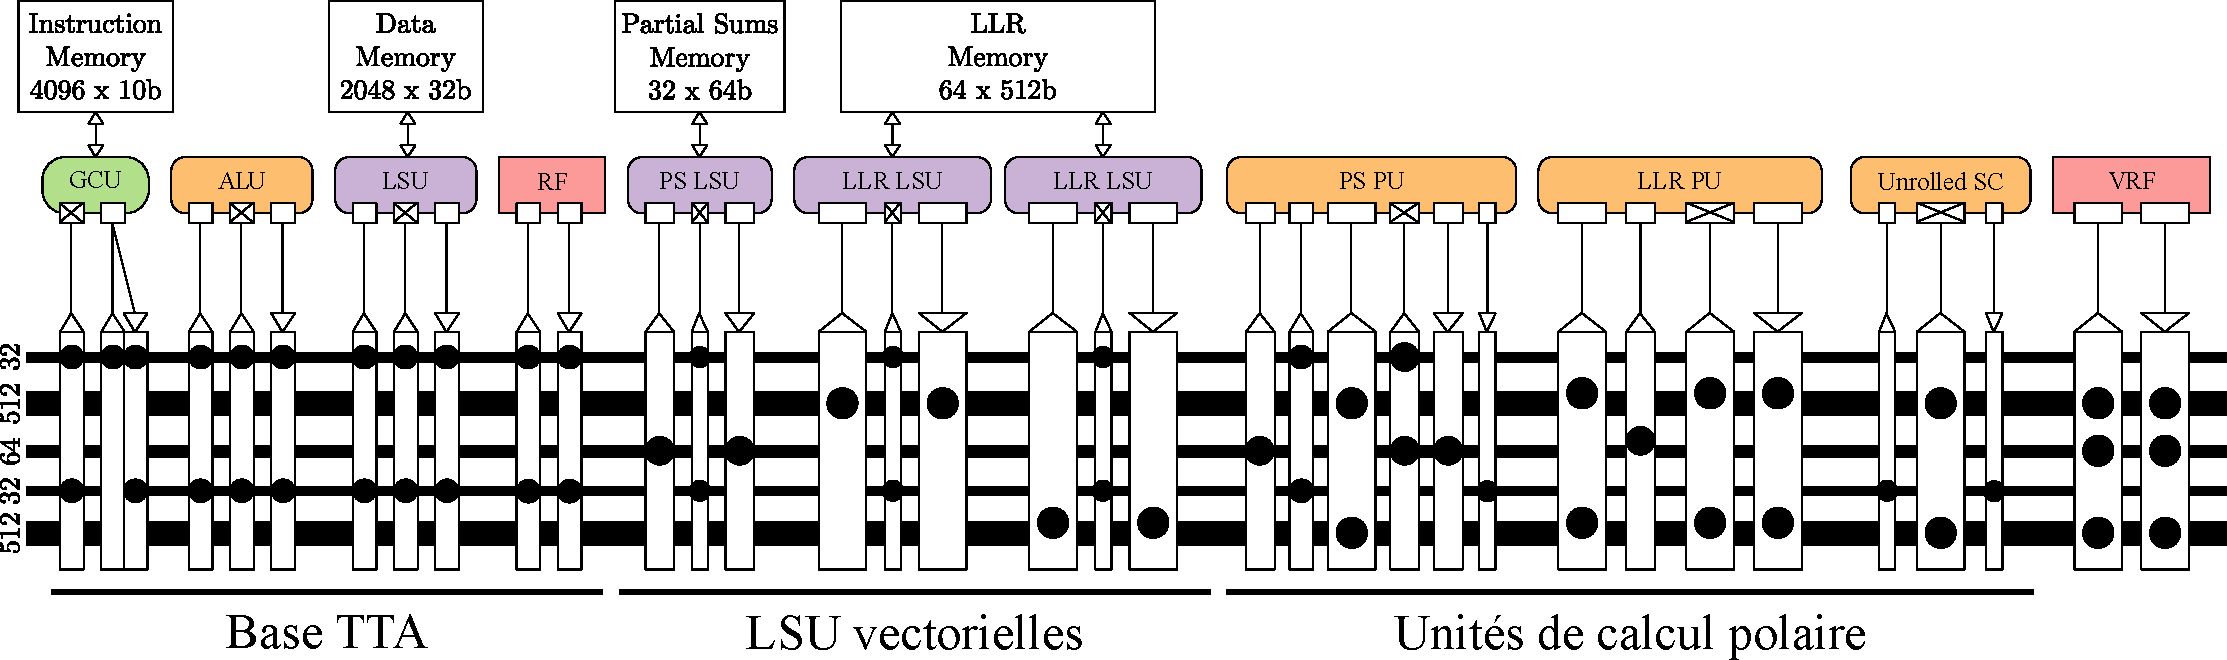
\includegraphics[width=\textwidth]{main/ch4_fig/archi_sc}
	\caption{Architecture \TTSC.}
	\label{fig:prode}
\end{figure*}

L'architecture \TTSC est divisée en trois parties principales. La Base TTA contient les unités fonctionnelles de base permettant de réaliser les fonctions d'un processeur généraliste. Elle est constituée d'une unité de chargement et de sauvegarde (LSU : Loading and Storing Unit), d'une ALU et d'un fichier de registres. Elle contient également l'unité de contrôle global (GCU : Global Control Unit) qui est destinée à la lecture et au décodage des instructions. La seconde partie est constituée des LSU vectorielles. Elles se chargent du chargement et de la sauvegarde des données vers et depuis les mémoires contenant les LLRs et les sommes partielles.
La troisième partie contient les unités de calcul (PU : Processing Unit), dont le but est de réaliser les fonctions élémentaires polaires.

Les algorithmes de décodages de codes polaires sont très intensifs du point de vus des accès à la mémoire. Les architectures matérielles dédiées de la littératures utilisent en majorité deux mémoires séparées pour accéder aux LLRs et deux autres pour les sommes partielles. Pour l'opération $f$, il est par exemple nécessaire d'effectuer deux lectures en mémoire ainsi qu'une écriture. Ces nombres sont à multiplier par le parallélisme, soit $P=64$. Les mêmes lectures et écritures sont nécessaires pour la fonction $g$, auquelles il faut ajouter la lecture de 64 sommes partielles. Dans l'architecture \TTSC, nous avons choisi d'utiliser une mémoire double port pour stocker les LLRs. Cela permet d'augmenter la bande passante, tout en conservant un seul espace de mémoire pour l'ensemble des LLRs. A chaque port est associé une LSU.

Les trois unités de calcul polaires sont l'unité de calcul de sommes partielles (PS PU), l'unité de calcul des LLRs (LLR PU) et l'unité \og SC déroulé \fg. La PS PU réalise les calculs des fonctions \texttt{R0}, \texttt{R1} et \texttt{h}. La LLR PU réalise les calculs des fonctions $f$ et $g$. L'unité \og SC déroulé \fg permet le décodage multicycle de sous-arbres. Elle sera détaillée par la suite. 

Le nombre d'unités fonctionnelles utilisées dans une architecture TTA est un choix important du concepteur.
Il s'agit d'un compromis.
Tout d'abord, une unité fonctionnelle ne peut activer qu'une opération à la fois.
Augmenter le nombre de FUs est donc nécessaire pour bénéficier du parallélisme d'instructions
Cela permet également d'augmenter la modularité de l'architecture du point de vue du concepteur.
\`A fonctionnalité égale, utiliser un grand nombre de FUs implique que chaque FU est plus simple, car elle doit réaliser moins d'opérations. Les modèles matériels sont donc plus simples à décrire, à modifier et à faire évoluer. Il est également plus probable de pouvoir réutiliser une FU simple dans de futures architectures.

En revanche le nombre de ports augmente avec le nombre de FUs, ainsi que le nombre de connexions nécessaires sur le réseau d'interconnexion.
Au niveau de l'implémentation, la densité du réseau d'interconnexion devient rapidement un problème. 
La congestion peut provoquer une augmentation du chemin critique et de la fréquence. 
Au cours du développement de l'architecture \TTSC, il a été nécessaire de fusionner des FUs afin de réduire la congestion et d'augmenter la fréquence d'horloge, au prix d'une réduction de la modularité et d'une augmentation de la complexité des FUs. La PS PU est par exemple la fusion de trois FUs de versions antérieures de l'architecture.

Le réseau d'interconnexion possède deux bus de 512 bits pour le transport des LLRs, un bus de 64 bits pour le transport des sommes partielles, et deux bus de 32 bits pour le transports des données génériques et des adresses.
Dans la section suivantes, certaines des FUs sont détaillées.

\subsection{Unités fonctionnelles du décodeur \texttt{TT-SC}.}
Nous allons détailler ici la fonction et l'implémentation matérielles de certaines des FUs. Toutes ne seront pas détaillées. Certaines (GCU, ALU, LSU, RF) sont liées au fonctionnement du base du TTA et à ce titre ne sont pas pertinentes ici. D'autres (LLR PU, PS PU) sont très similaires aux instructions spécialisées de l'architecture Tensilica du chapitre \ref{chap:tensilica}, décrites dans la sous-section \ref
{subsec:multi_reg}.

Les unités fonctionnelles originales spécifiques à cette architectures sont les unités de chargement et de sauvegarde vectorielles d'une part, et l'unité \og SC déroulé \fg d'autre part.

\subsubsection{Unités de chargement et de sauvegarde.}

\begin{figure*}[t]
	\centering
	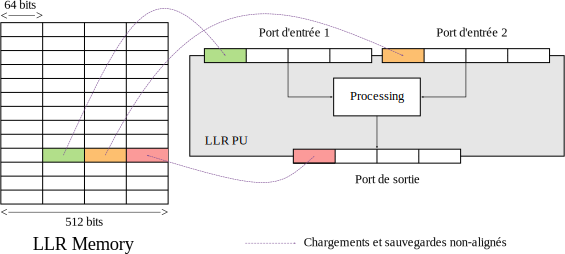
\includegraphics[width=\textwidth]{main/ch4_fig/unaligned}
	\caption{Chargements et sauvegardes non alignés.}
	\label{fig:unaligned}
\end{figure*}


Les unités de chargement et de calcul vectoriels permettent d'accéder aux mémoires contenant les LLRs et les sommes partielles. Dans l'architecture proposée, la taille de code maximum supportée est $N_{max}=1024$, qui correspond à la taille maximum définie dans le standard 5G \cite{3gpp_ts_2017}. Cette valeur peut être facilement ajustée en augmentant la taille des mémoires. Dans l'algorithme SC, $N_{max}$ bits sont nécessaires pour stocker les sommes partielles. Puisqu'il est nécessaire d'accéder à $P=64$ sommes partielles en parallèle, une mémoire de 16 x 64-bits est suffisante. Cependant, à cause d'une section d'adresse réservée automatiquement par TCE, une taille supérieure de mémoire a due être sélectionnée : 32x64-bits. Pour des raisons similaires, les LLRs sont stockés dans une mémoire de 64x512-bits.

Comme précisé auparavant, l'accès à la mémoire est un enjeu capital dans les architectures de décodage de codes polaires. Les modèles architecturaux et matériels de LSU proposés par défaut dans les bases de données de TCE ont une latence de 3 cycles d'horloge, ce qui est trop élevé. Dans un premier temps, cette latence a été réduite à un coup d'horloge par la suppression de registres. Cette suppression n'a pas causé d'augmentation du chemin critique.

La deuxième amélioration apportée à ces LSU est l'ajout d'unités matérielles et d'opérations d'alignement. En effet, pour effectuer parallèlement le traitement de certaines portions de l'arbre de décodage pour lequel le parallélisme est inférieur à $P$, il est nécessaire de lire et d'écrire sur des données non alignées. Les données non alignées sont des données dont l'adresse n'est pas un multiple de 512, dans le cas des LLRs, ou de 64, dans le cas des sommes partielles. De plus les mots en mémoire sont des mots de 512 bits. Dans les portions de l'arbre à parallélisme inférieur à $P$, il est nécessaire d'écrire des sous-mots de taille inférieure à 512 bits (jusqu'à 64 bits). D'une part, il est nécessaire que les mémoires gèrent ces écritures de sous-mots. D'autre part, les LSUs doivent être capables d'effectuer le contrôle de ces mémoires. Le processus de chargement et de sauvegarde de données non alignées est illustré dans la Figure \ref{fig:unaligned}.

\subsubsection{Décodage d'un sous arbre déroulé multi-cycles.}

\begin{figure*}[t]
	\centering
	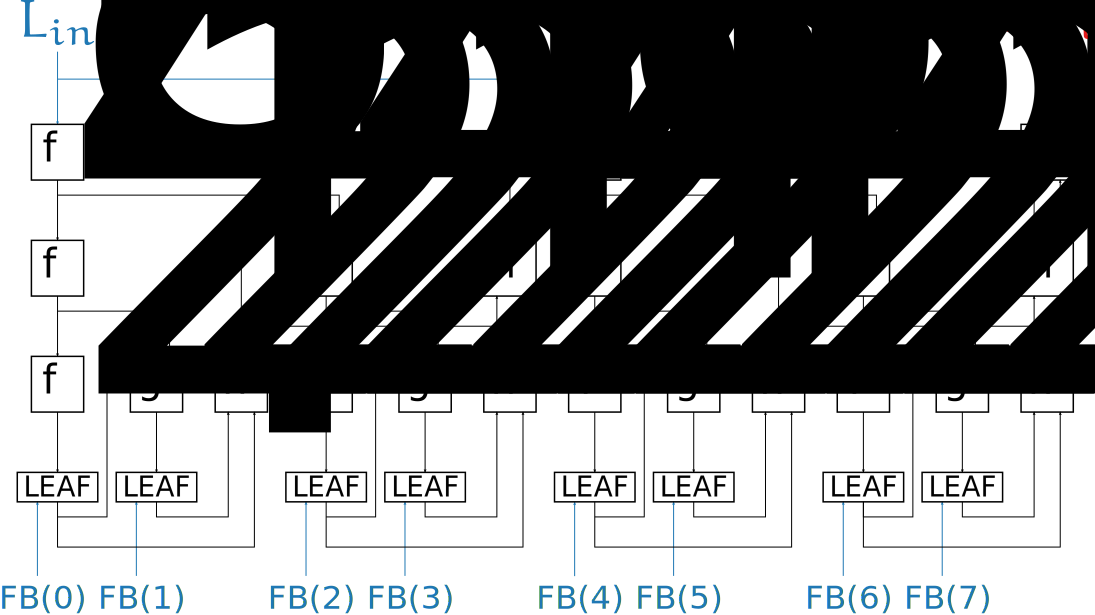
\includegraphics[width=\textwidth]{main/ch4_fig/unrolled_multicycle}
	\caption{Unité matérielle de décodage d'un sous arbre déroulé multi-cycles.}
	\label{fig:unrolled_multicycle}
\end{figure*}

Dans \cite{gal_scalable_2016} est proposé une architecture matérielle de codes polaires à plusieurs phases. Les différentes phases correspondent à différents ensembles de niveaux de l'arbre de décodage. Trois différentes techniques sont appliqués pour les niveaux supérieurs, les niveaux inférieurs et les niveaux inférieurs. La phase qui nous intéresse ici est la phase de décodage des niveaux inférieurs. Considérons les sous-arbre dont le \noeud racine contient 8 LLRs. Ce sous-arbre est de taille réduite. Aussi, il est possible de le dérouler complètement. Il est montré que ce déroulage permet de réduire le nombre de cycles nécessaires. En effet, la durée de cette séquence de décodage avec une architecture semi-parallèle classique serait de 14 cycles. En déroulant l'arbre de décodage et en découpant le chemin combinatoire à l'aide de registres, la latence obtenue est de six cycles. Cette technique s'inspire de la technique \cite{giard_unrolled_2015} à la différence qu'ici, le décodeur déroulé n'est pas pipeliné et le but des registres est simplement de découper le chemin critique. Comme il n'y a pas de pipelinage, il est donc possible de supprimer les registres et de définir le chemin de données allant du début à la fin du sous-arbre de décodage comme un chemin multi-cycles.

En effet, il est possible de définir des chemins de données multi-cycles dans les processeurs conçus à l'aide de TCE. Dans TCE, par défaut, la latence d'une opération effectuée dans une FU est d'un cycle d'horloge : lorsqu'à un front d'horloge, une donnée est présentée au port de déclenchement, les résultats de l'opération sont disponibles aux ports de sortie au front d'horloge suivant. Dans l'outil \textbf{prode}, qui permet de définir l'architecture, il est toutefois possible d'assigner une latence supérieure à une ou plusieurs opérations d'une FU. Si une latence supérieure est spécifiée, alors les données de sortie ne seront disponibles qu'après le nombre spécifié de coups d'horloge. Le compilateur a connaissance de cette latence spécifiée dans le fichier \textit{.adf}. Il est ainsi en charge de régler les problèmes de disponibilités des données. Du côté du logiciel tiers de synthèse, il est alors possible de spécifier que les chemins de données de l'opération en question sont multicycles. La contrainte de temps ceux-ci est allongée de plusieurs cycle d'horloge. Ainsi, les registres sont supprimés, et la complexité matérielle de l'unité est réduite. Potentiellement, cette technique pourrait réduire le nombre de cycles nécessaires au décodage du sous-arbre par rapport à la version contenant les registres. Toutefois, dans notre implémentation, le nombre de cycles n'a pas été réduit par rapport à l'implémentation de \cite{gal_scalable_2016}. Une des raisons possibles est que dans notre décodeur, comme dans l'ASIP d'architecture Tensilica, les nombres entiers signés sont représentés en complément à deux. La représentation signe-magnitude utilisée dans \cite{gal_scalable_2016} permet de simplifier le traitement de la fonction $f$.

L'unité fonctionnelle \og SC déroulé \fg correspond donc à un sous-arbre de décodage SC déroulé et multi-cycles. Ce sous-arbre est représenté dans la Figure \ref{fig:unrolled_multicycle}. Il est important de noter que les bits gelés sont donnés en entrée du sous-arbre. Ceci lui permet d'être générique vis-à-vis du rendement et de la construction du code.



\subsection{Description logicielle}
\subsection{Implémentation de l'algorithme SCAN}
Afin d'illustrer la modularité et l'évolutivité des processeurs d'architecture TTA conçus à l'aide de TCE, nous avons développé une nouvelle architecture nommée \TTSCAN. Elle permet le support de l'algorithme SCAN en plus de l'algorithme SC. La Figure \ref{fig:tt_scan} représente cette nouvelle architecture.


\section{Un flot de conception complet}

\subsection{Génération des vecteurs de tests}
\subsection{Cycles de conception}

\section{Expérimentations et mesures}

\subsection{TT-SC}
\subsection{TT-SCAN}


\section*{Conclusion}


             % Troisième thème (Doctorat) ou effacez ce fichier si vous êtes à la Maîtrise.
%!TEX root = ../my_thesis.tex
\chapter*{Conclusions et perspectives}
\markboth{Conclusions et perspectives}{Conclusions et perspectives}
\addcontentsline{toc}{chapter}{Conclusions et perspectives}

\section*{Avantages et inconvénients de chaque approche}
\section*{Conclusions}
Dans le deuxième chapitre, des implémentations logicielles des algorithmes de codes polaires à liste sont proposées. L'originalité de ces implémentations tient à leur forte flexibilité. Cette flexibilité est inédite en comparaison des travaux publiés dans la littérature sur le même sujet. Tout d'abord, les données internes de l'algorithme sont représentées en virgule fixe, ce qui diminue l'empreinte mémoire et permet de réduire le temps nécessaire au décodage d'une trame. De plus, l'élagage de l'arbre de décodage est une simplification indispensable pour atteindre de hauts débits et de faibles latences de décodage. Cet élagage, dans les décodeurs proposés, est dynamiquement configurable. La flexibilité de l'élagage permet des compromis intéressants entre débit, latence et performance de décodage. Grâce à différentes optimisations, la flexibilité et la généricité du décodeur sont atteintes sans sacrifier le débit ou la latence de décodage. Une des versions de l'algorithme à liste, l'algorithme FASCL, permet même de dépasser le débit des implémentations de l'état de l'art sur les architectures x86. Des résultats d'implémentation des algorithmes de décodage de codes polaires à liste sont également proposés sur des architectures ARM. Les débits sont moindres, mais la consommation énergétique est réduite.

Dans le troisième chapitre, une architecture de processeur spécialisée pour le décodage de codes polaires est proposée. Le processeur fait partie de la famille des ASIP. Les outils de la marque Tensilica sont utilisés. Les processeurs conçus à l'aide des ces outils sont des processeurs de type RISC, dont le jeu d'instructions est étendu et la microarchitecture modifiée afin de les rendre plus efficaces pour une application donnée. Ils conservent toutefois la versatilité de architectures RISC classiques, et bénéficient d'un écosystème logiciel facilitant leur conception et le développement de programme les ciblant. Tout comme les implémentations du chapitre précédent, le programme est décrit logiciellement, dans un langage de haut niveau (C, C++, OpenCL). Les expérimentations et les mesures réalisées montrent que l'architecture de processeurs proposée permet d'atteindre des débits comparables à ceux obtenus sur les architectures ARM, tout en réduisant la consommation énergétique d'un ordre de grandeur.

Dans le quatrième chapitre, une architecture de processeur de type TTA est conçue. Configurable plus finement et d'une structure plus modulaire, ce type d'architecture se rapproche des implémentations matérielles dédiées, du point de vue de leur structure comme de celui de leurs performances. Tout comme les architectures du chapitre troisième, elles n'en restent pas moins versatiles et programmables. Elles sont également dotées d'un environnement de conception complet. Cet environnement est une suite logicielle libre développée par l'équipe \og Customized Parallel Computing \fg de l'université technique de Tampere (TUT). Contrairement aux architectures réalisées avec les outils de Tensilica, le modèle complet du processeur est produit par l'environnement, pour être utilisé par des logiciels de synthèse tiers. Deux architectures sont proposées. La première supporte l'algorithme SC seul. La seconde supporte les algorithmes SC et SCAN. Les deux sont synthétisées et implantées sur des circuits FPGA. Les résultats de synthèse de la première architecture montrent qu'elle permet de surpasser les débits obtenus sur les architectures x86, tout en réduisant la consommation énergétique de deux ordres de grandeur.

Dans le Tableau \ref{tab:synthesis}, les caractéristiques des différentes architectures de décodage considérées dans ce manuscrit sont présentées. Tout d'abord, les processeurs d'architecture x86-64 et ARM sont disponibles sur le marché. Au contraire, les ASIP sont des architectures spécialisées pour lequel des frais doivent être engagées afin d'en réaliser l'implantation sur cible ASIC. Cependant, les deux ASIP sont plus efficaces énergétiquement. L'architecture \texttt{TT-SC} est la plus performante du point de vue du débit et de l'efficacité énergétique. Néanmoins, il s'agit aussi de l'architecture la moins généraliste. Un des symptômes de ce manque de flexibilité et l'absence de système d'exploitation ciblant les architectures TTA, tandis que les processeurs XTensa bénéficient d'un système d'exploitation fondé sur le noyau Linux. En effet, les processeurs XTensa sont basés sur des architectures RISC qui sont des architectures de processeurs classiques. En ce sens, sa flexibilité se rapprochent de celles des architectures x86-64 et ARM.
L'ensemble des quatre architectures de processeurs offre des compromis marqués entre flexibilité, performance et efficacité énergétique.

\begin{table}[htp]
\centering
\caption{Existence, disponibilité d'un système d'exploitation, débits et consommation énergétiques des processeurs pour les différentes architectures considérées. Les intervalles de débit et de consommation énergétique concernent le décodage de mots de codes polaires dont les tailles varient de $N=128$ à $N=1024$ et dont le rendement est $R=1/2$}
\label{tab:synthesis}
{\small\resizebox{\linewidth}{!}{
 \begin{tabular}{r|cccc}
  \multirow{1}{*}{\textbf{Architecture}}  & \textbf{Processeur}  & \textbf{Système}        & $\bm{\mathcal{T}_i}$  & $\bm{\mathcal{E}_b}$ \\
                                          & \textbf{existant}    & \textbf{d'exploitation} & \textbf{Mb/s}         & \textbf{Mb/s}        \\
  \cmidrule(lr){1-1}
  \cmidrule(lr){2-2}
  \cmidrule(lr){3-3}
  \cmidrule(lr){4-4}
  \cmidrule(lr){5-5}
  
  x86-64 (Haswell)                        & \cmark              & \cmark                   & 120-260                 & 40-90              \\
  ARMv8-A                                 & \cmark              & \cmark                   & 30-40                   & 10-30              \\
  XTensa Polaire                          & \xmark              & \cmark                   & 30-70                   & 1-2                \\
  \texttt{TT-SC}                          & \xmark              & \xmark                   & 250-350                 & 0.1-0.2            \\
\end{tabular}
}}
\end{table}

%\multirow{1}{*}{\textbf{Débit}} 
\section*{Perspectives}

Le décodeur logiciel proposé dans le chapitre \ref{chap:soft_scl} fait partie du projet AFF3CT de l'équipe CSN du laboratoire IMS de Bordeaux. Le but de ce projet est de proposer à la communauté scientifique des implémentations logicielles efficace d'algorithmes de décodage de codes correcteurs d'erreurs. Les travaux réalisés dans le cadre de cette thèse l'ont grandement enrichi. Dans le futur, une plus grande variété d'algorithmes de décodage de codes polaires pourrait être supportée. Par exemple, les algorithmes SCF et SCS présentés dans le chapitre \ref{chap:soft_scl} présentent un intérêt certains. Cependant, pour autant que nous le sachions, il n'existe aucune référence dans la littérature reportant les débits et les latences obtenus sur des architectures de processeur à usage général. Or, la faible complexité calculatoire de l'algorithme SCF semble indiquer de bonnes performance potentielles dans ce domaine, malgré des performances de décodage légèrement en retrait de l'algortihme SCL. L'algorithme SCS présente quant à lui des performances de décodage égales à celles de l'algorithme SCL. Des travaux récents tendent à montrer que de hauts débit et de faibles latences pourraient être atteints \cite{8351832}.

Parmi les architectures considérées dans ces travaux, celles permettant d'atteindre les meilleurs débits, latences et efficacités énergétiques sont les architectures TTA. Un axe de recherche envisagé est la conception d'une architecture TTA pour le décodage des algorithmes de codes polaires à liste. En effet, les performances de décodage sont bien plus élevées, au prix d'une plus grande complexité calculatoire. Plusieurs étapes seront nécessaires. Tout d'abord, nos travaux montrent que le temps alloué à la propagation des sommes partielles doit être réduit. Une solution pourrait être de s'inspirer de ce qui est réalisé dans les architectures matérielles dédiées. Ensuite l'architecture devra être étendue, afin de permettre le parcours de plusieurs arbres de décodage en parallèle, ainsi que la gestion des métriques de chemin. La flexibilité de l'architecture pourra alors être mise à profit afin de gérer un large panel de codes polaire saux caractéristiques variées, tels que ceux définis dans le standard 5G.

Enfin, la suite logicielle TCE facilite la conception de plateformes multicœurs. Des travaux récents montrent les gains potentiels de ces architectures en termes de débit pour des turbo codes \cite{kultala_turbo_2013}. Des problématiques de dimensionnement du nombre de cœurs, des interfaces et des mémoires doivent être relevées pour créer de tels systèmes.
         % Conclusion.
%\backmatter
\ifthenelse{\equal{\Langue}{english}}{
	\renewcommand\bibname{BIBLIOGRAPHY}
	\bibliography{tail/bibliography}
	\bibliographystyle{IEEEtran}			% Bibliography style.
}{
	\renewcommand\bibname{RÉFÉRENCES}
	\bibliography{tail/bibliography}
	\bibliographystyle{IEEEtran-francais}    % Style de la bibliographie.
	\bibliographystylemine{IEEEtran-francais}
	\bibliographymine{tail/bibliography}
}
%
\ifthenelse{\equal{\AnnexesPresentes}{O}}{
	\appendix%
	\newcommand{\Annexe}[1]{\annexe{#1}\setcounter{figure}{0}\setcounter{table}{0}\setcounter{footnote}{0}}%
	%!TEX root = ../my_thesis.tex

\appendix
\chapter{Compléments au Chapitre Premier}
\section{Détails des calculs de l'algorithme APP}\label{append:app}
Cette partie vise à démontrer l'ensemble des calculs présentés dans la section \ref{sec:BCJR}.
\subsection{Décomposition de la probabilité jointe} 
Cette décomposition est basée sur le partitionnement de la séquence reçue $\mathbf{y}$ en trois sous-séquences. La première représentant le passé $ \mathbf{y_{<k}}$, la seconde le présent $\mathbf{y_{k}} $ et enfin le futur $ \mathbf{y_{>k}}$.

Le calcul suivant est basé sur la relation de Bayes : $P(A|B) = \frac{P(A,B)}{P(B)}$ et sa version ternaire $P(A|B,C) = \frac{P(A,B|C)}{P(B|C)}$.

Aussi, sont nécessaires au déroulement de ce calcul les propriétés de Markov du treillis de l'encodeur RSC considéré. En effet :
\begin{align*}
	\hspace*{-4ex}
	P(s_{k-1}=s, s_{k}=s',\mathbf{y}) & = P(s_{k-1}=s, s_{k}=s',\mathbf{y_{<k}},\mathbf{y_{k}},\mathbf{y_{>k}})                                                                                                                             \\
	                                  & = P(\mathbf{y_{>k}}|s_{k-1}=s, s_{k}=s',\mathbf{y_{<k}},\mathbf{y_{k}})\times P(s_{k-1}=s, s_{k}=s',\mathbf{y_{<k}},\mathbf{y_{k}})                                                                 \\
	                                  & =P(\mathbf{y_{>k}}|s_{k}=s')\times P(s_{k-1}=s, s_{k}=s',\mathbf{y_{<k}},\mathbf{y_{k}})                                                                                                            \\
	                                  & =P(\mathbf{y_{>k}}|s_{k}=s')\times P(s_{k}=s',\mathbf{y_{k}}|s_{k-1}=s,\mathbf{y_{<k}})\times P(s_{k-1}=s,\mathbf{y_{<k}})                                                                          \\
	                                  & = \underbrace{P(\mathbf{y_{>k}}|s_{k}=s')}_{\beta_k(s')}\times \underbrace{P(s_{k}=s',\mathbf{y_{k}}|s_{k-1}=s)}_{\gamma_k(s,s')}\times \underbrace{P(s_{k-1}=s,\mathbf{y_{<k}})}_{\alpha_{k-1}(s)} \\
	                                  & = \alpha_{k-1}(s) \times \gamma_k(s,s') \times \beta_k(s')                                                                                                                                          
\end{align*}

\subsection{Calcul récursif de $\alpha$}
Par définition, $\alpha_{k-1}(s) = P(s_{k-1}=s,\mathbf{y_{<k}})$. Or, sachant que $\sum\limits_B P(A,B) = P(A)$ et en appliquant le théorème de Bayes,
\begin{align*}
	\hspace*{-4ex}
	\alpha_k(s) & = \sum\limits_{s'}P(s_{k}=s,s_{k-1}=s',\mathbf{y_{<k}},\mathbf{y_k})                                        \\
	            & = \sum\limits_{s'}P(s_{k}=s,\mathbf{y_k} | s_{k-1}=s',\mathbf{y_{<k}}) \times P(s_{k-1}=s',\mathbf{y_{<k}}) \\
	            & = \sum\limits_{s'}P(s_{k}=s,\mathbf{y_k} | s_{k-1}=s') \times P(s_{k-1}=s',\mathbf{y_{<k}})                 \\
	            & = \sum\limits_{s'}\gamma_k(s',s)\times \alpha_{k-1}(s')                                                     
\end{align*}
Ainsi, les valeurs de $\alpha_k(s)$ peuvent être calculées récursivement en parcourant le treillis dans l'ordre chronologique, à partir des valeurs initiales $\alpha_0(s)$ et des probabilités de transition.

\subsection{Calcul récursif de $\beta$}
En utilisant les mêmes propriétés calculatoires que pour le calcul de $\alpha$ : 
\begin{align*}
	\hspace*{-4ex}
	\beta_{k-1}(s) & = P(\mathbf{y_{>k-1}}|s)                                                             \\
	               & = \sum\limits_{s'}P(s',\mathbf{y_{k}},\mathbf{y_{>k}|s})                             \\
	               & = \sum\limits_{s'}P(\mathbf{y_{>k}} | s',s, \mathbf{y_{k}}) P(s', \mathbf{y_{k}}| s) \\
	               & = \sum\limits_{s'}P(\mathbf{y_{>k}} | s') P(s', \mathbf{y_{k}}| s)                   \\
	               & = \sum\limits_{s'}\gamma_k(s,s')\times \beta_{k}(s')                                 
\end{align*}


\subsection{Calcul de la probabilité \textit{a posteriori}}
La probabilité \textit{a posteriori} a pour expression : 
\begin{align*}
	\|\mathbf{y}_k-\mathbf{c}_k\|^2 & = (y_k^s - c_k^s)^2 + (y_k^p - c_k^p)^2                                               \\
	                                & = (y_k^s)^2 - 2  y_k^s   c_k^s +  (c_k^s)^2 + (y_k^p)^2 - 2  y_k^p c_k^p +  (c_k^p)^2 \\
	                                & = (y_k^s)^2 +   (y_k^p)^2 + 2  - 2*( y_k^s   c_k^s +  y_k^p c_k^p)                    
\end{align*}

Ainsi, \[\gamma_k(s,s') = \frac{P(m_k)}{2\pi\sigma^2}\exp\left(-\frac{ (y_k^s)^2 +   (y_k^p)^2 + 2}{2\sigma^2}\right) \exp\left(\frac{( y_k^s   c_k^s +  y_k^p c_k^p)}{\sigma^2}\right)\]

Or, la première exponentielle n'est pas dépendante de $m_k$ (ou du chemin $ s \mapsto s'$) et peut donc être supprimé du numérateur et du dénominateur dans l’expression de la probabilité \textit{a posteriori}.


\section{Détails des calculs pour les algorithmes sub-APP}\label{append:subAPP}
\subsection{Calcul des métriques}
Dans le cadre des algorithmes sub-APP, les probabilités manipulées sont transformées en métriques en prenant le logarithme népérien de celles-ci. Ainsi, nous avons :
\begin{align*}
	\tilde{\alpha}_k(s) & = \ln \sum\limits_{s'}\alpha_{k-1}(s')\times\gamma_k(s',s)                                                     \\
	                    & = \ln \sum\limits_{s'} \exp\left(\tilde{\alpha}_{k-1}(s')\right)\times\exp\left(\tilde{\gamma}_k(s', s)\right) \\
	                    & = \ln \sum\limits_{s'} \exp\left(\tilde{\alpha}_{k-1}(s') + \tilde{\gamma}_k(s', s)\right)                     
\end{align*}
Des calculs très similaires permettent d'obtenir $\tilde{\beta}_k(s)$ et $\tilde{\gamma}_k(s,s')$.

\subsection{Opérateur $\maxstar$}\label{append:maxstar}
En partant de la définition de l’opérateur $\maxstar$ et en utilisant une disjonction de cas, on obtient : 
\begin{align*}
	\maxstar(x,y) & = \ln\left(\e^x+\e^y\right)              \\
	              & =\begin{cases}                           
	\ln	\left(\e^x\left(1+\e^{y-x}\right)\right) \text{si} x>y  \\
	\ln	\left(\e^y\left(1+\e^{x-y}\right)\right) \text{si} x<y
	\end{cases}\\
	              & =\begin{cases}                           
	x + \ln\left(1+\e^{y-x}\right) \quad\text{si}\quad x>y  \\
	y+\ln\left(1+\e^{x-y}\right) \quad\text{si}\quad x<y
	\end{cases}\\
	              & =\max(x,y) +\ln\left(1+\e^{|x-y|}\right) 
\end{align*}


% Ainsi, en reprenant les définitions récursives et en substituant les probabilités par les métriques, leurs expressions deviennent : 
% \begin{align*}
% 	M^\alpha_k(s) & = \ln \sum\limits_{s'}\alpha_{k-1}(s')\times\gamma_k(s',s)                                         \\
% 	              & = \ln \sum\limits_{s'} \exp\left(M^\alpha_{k-1}(s')\right)\times\exp\left(M^\gamma_k(s', s)\right) \\
% 	              & = \ln \sum\limits_{s'} \exp\left(M^\alpha_{k-1}(s') + M^\gamma_k(s', s)\right)                     
% \end{align*}
% et 
% \[M^\beta_k(s) = \ln \sum\limits_{s'} \exp\left(M^\beta_{k+1}(s') + M^\gamma_{k+1}(s, s')\right)\]
% avec pour conditions initiales, 

% De même les LLR \textit{a posteriori} deviennent :
% \begin{align*} 
% 	L(m_k) & = \ln \sum\limits_{s,s'\in S_1} \exp\left( M^\alpha_{k-1}(s) + M^\gamma_{k}(s, s') + M^\beta_k(s') \right)       \\ 
% 	       & \quad - \ln \sum\limits_{s,s'\in S_0} \exp\left( M^\alpha_{k-1}(s) + M^\gamma_{k}(s, s') + M^\beta_k(s') \right) 
% \end{align*}
% Toutefois, ces réécritures dans le domaines logarithmiques ne permettent pas encore de réduire la complexité calculatoire. Pour ce faire, introduisons l'opérateur \[\maxstar(x,y) = \ln(\mathrm{e}^x + \mathrm{e}^y).\]
% Ainsi, les métriques précédentes deviennent : 



% Il est démontré facilement (en utilisant un disjonction de cas) que :
% \[\maxstar(x,y) = \max(x,y) + \ln(1+e^{|x-y|})\]
% \paragraph{Stabilité numérique}


\chapter{Compléments au Chapitre Deuxième}
\section{Standard CCSDS}\label{sec:annCCSDS}
Cette section présente les observations statistiques obtenues avec le standard CCSDS. La Figure \ref{fig:m_ccsds} présente 
les valeurs moyennes d'oscillations, ce pour différentes valeurs de SNR. Les Figures \ref{fig:it1_ccsds} et \ref{fig:it2_ccsds}
présentent l'évolution des oscillations au cours des itérations pour, respectivement, un taux d'erreur trame correspondant 
au seuil de convergence et un correspondant au plancher d'erreur. Finalement, les Figures \ref{fig:d1_ccsds} et \ref{fig:d2_ccsds} 
présentent la distribution normalisée des oscillations pour ces deux valeurs de SNR considérées.
\begin{figure}[tb]
	\begin{center}
	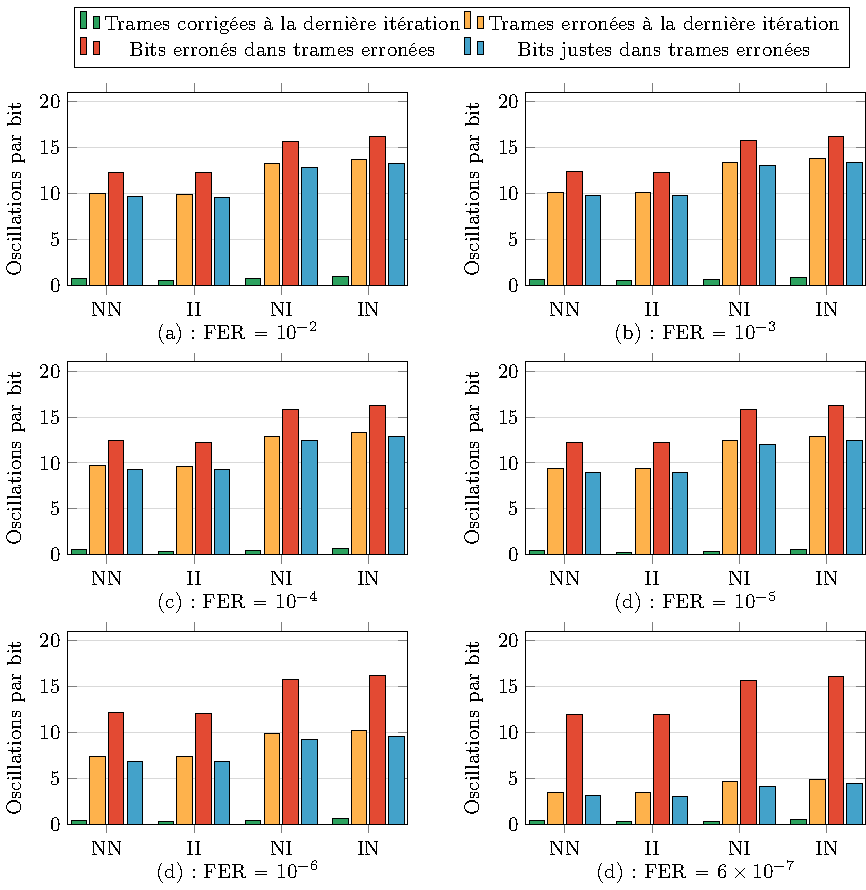
\includegraphics[width=.9\textwidth]{main/ch2_fig/tikz/m_ccsds.pdf}
	\caption{Nombre moyen d'oscillations pour différents taux d'erreurs trame cibles, turbo code du standard CCSDS (K=1784, R=1/3) \label{fig:m_ccsds}}
	\end{center}
\end{figure}

\begin{figure}[!ht]
	%\hspace*{-.7cm}	
	\begin{center}
	\includegraphics[width=.9\textwidth]{main/ch2_fig/tikz/it_ccsds10-2.pdf}
	\caption{Oscillations au cours des itérations dans le cadre du standard CCSDS (K=1784, R=1/3) pour un taux d'erreur trame de $10^{-2}$\label{fig:it1_ccsds}}
	\end{center}
\end{figure}

\begin{figure}[!ht]
	%\hspace*{-.7cm}
	\begin{center}
	\includegraphics[width=.9\textwidth]{main/ch2_fig/tikz/it_ccsds610-7.pdf}
	\caption{Oscillations au cours des itérations dans le cadre du standard CCSDS (K=1784, R=1/3) pour un taux d'erreur trame de $6\times10^{-7}$\label{fig:it2_ccsds}}
	\end{center}
\end{figure}

\begin{figure}[!ht]
	\centering
	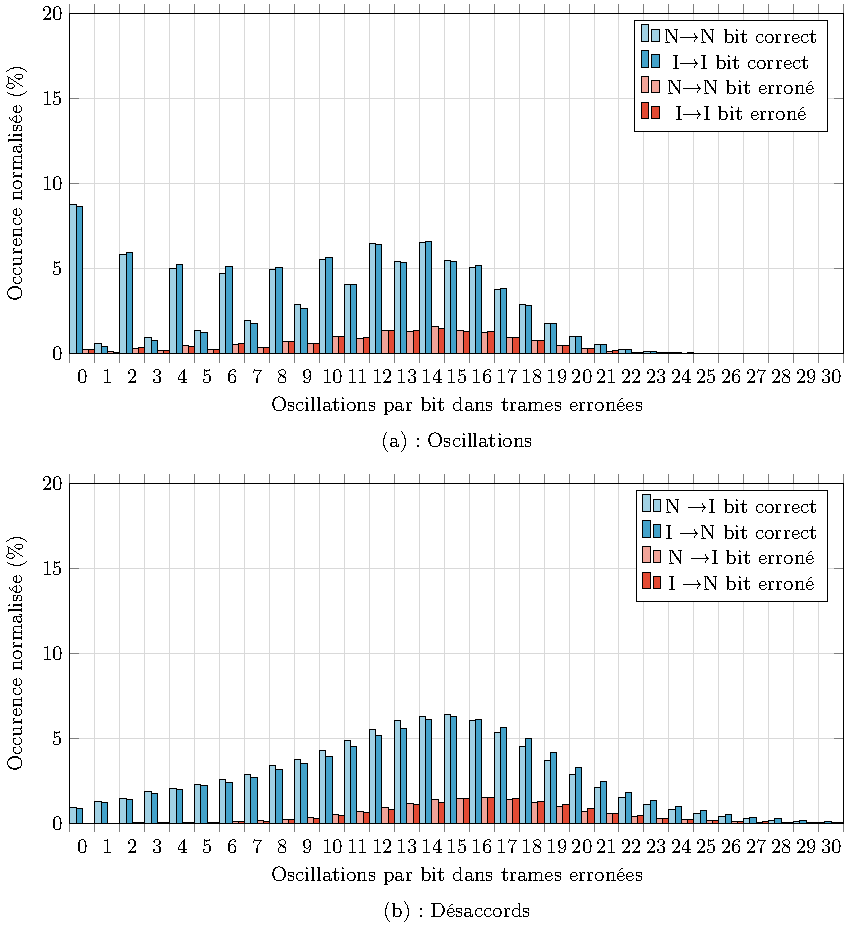
\includegraphics[width=.9\textwidth]{main/ch2_fig/tikz/d_ccsds_10-2.pdf}
	\caption{Distribution du nombre d'oscillations par bit pour un taux d'erreur trame de $10^{-2}$, pour le turbo code du standard CCSDS (K=1784, R=1/3)\label{fig:d1_ccsds}}
\end{figure}

\begin{figure}[!ht]
	\centering
	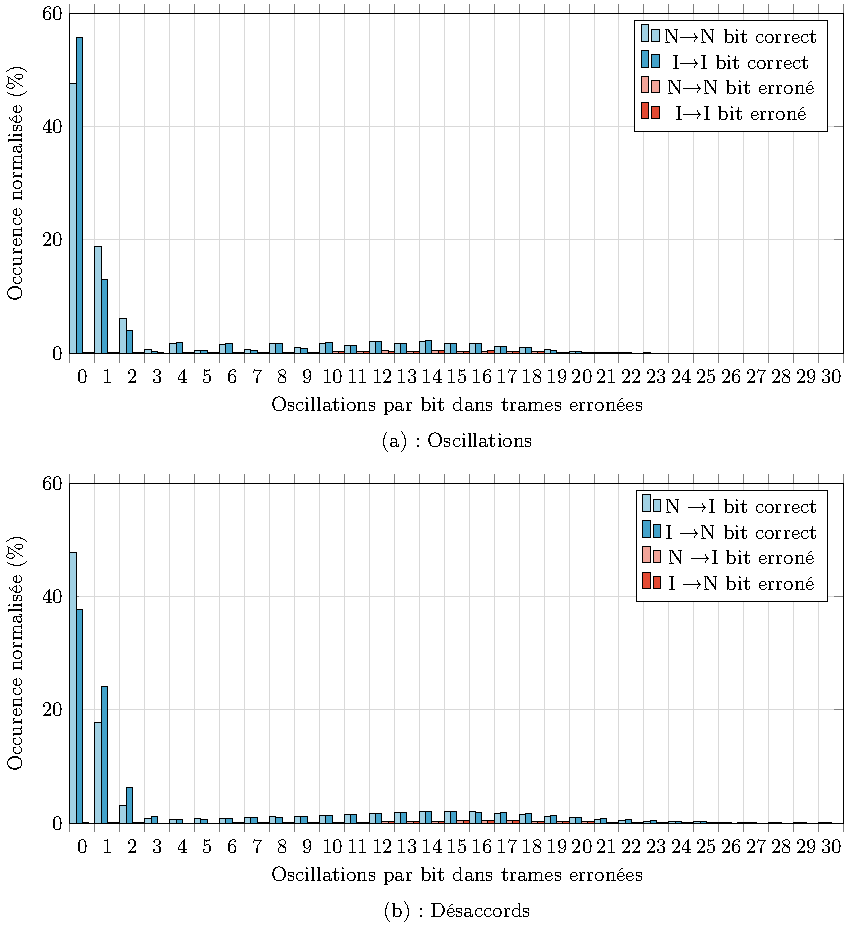
\includegraphics[width=.9\textwidth]{main/ch2_fig/tikz/d_ccsds_610-7.pdf}
	\caption{Distribution du nombre d'oscillations par bit pour un taux d'erreur trame de $6\times10^{-7}$, pour le turbo code du standard CCSDS (K=1784, R=1/3)\label{fig:d2_ccsds}}
\end{figure}


\chapter{Compléments au Chapitre Troisième}\label{sec:ann3}
\newpage
\begin{adjustbox}{angle=90}
\centering
\resizebox{1.5\textwidth}{!}{
\begin{tabular}{@{}llrrrrrrrrrrrrrrrrrrrrrrrrrrrr@{}}
\toprule
\multirow{15}{*}{\textbf{LTE}} & \multirow{3}{*}{\textbf{K=528}}  & \textbf{d} & 23 & 24 & 25 & 26 & 27 & 28 & 29 & 30 & 31 & 32 & 33 & 34 & 35 & 36 & 37   & 38   & 39    & 40   & 41  & 42  & 43   & 44   & 45   & 46  & 47   & 48  & 49  \\  
                    &    & \textbf{a} & 1  & 1  & 1  & 0  & 3  & 3  & 6  & 0  & 6  & 4  & 11 & 10 & 14 & 12 & 96   & 886  & 1421  & 45   & 123 & 156 & 192  & 227  & 140  & 55  & 285  & 52  & 62  \\
                    &    & \textbf{w} & 1  & 2  & 3  & 0  & 9  & 6  & 16 & 0  & 20 & 16 & 39 & 32 & 58 & 50 & 318  & 5268 & 12535 & 210  & 779 & 864 & 984  & 982  & 850  & 286 & 1415 & 260 & 292 \\ \cdashlinelr{2-30}
& \multirow{3}{*}{\textbf{K=1024}} & \textbf{d} & 27 & 28 & 29 & 30 & 31 & 32 & 33 & 34 & 35 & 36 & 37 & 38 & 39 & 40 & 41   & 42   & 43    & 44   & 45  & 46  & 47   & 48   & 49   &     &      &     &     \\
  &                      & \textbf{a} & 1  & 2  & 3  & 1  & 2  & 1  & 2  & 2  & 7  & 3  & 7  & 9  & 11 & 11 & 20   & 30   & 147   & 437  & 49  & 64  & 583  & 179  & 511  &     &      &     &     \\
   &                     & \textbf{w} & 1  & 4  & 9  & 2  & 6  & 2  & 6  & 6  & 21 & 12 & 27 & 32 & 43 & 44 & 78   & 142  & 719   & 1770 & 241 & 326 & 2949 & 1148 & 3407 &     &      &     &     \\ \cdashlinelr{2-30}
& \multirow{3}{*}{\textbf{K=1504}} & \textbf{d} & 25 & 26 & 27 & 28 & 29 & 30 & 31 & 32 & 33 & 34 & 35 & 36 & 37 & 38 & 39   & 40   & 41    & 42   & 43  & 44  & 45   & 46   & 47   & 48  & 49   &     &     \\
  &                      & \textbf{a} & 1  & 0  & 0  & 1  & 1  & 1  & 2  & 1  & 2  & 5  & 1  & 6  & 7  & 3  & 14   & 13   & 17    & 22   & 32  & 28  & 47   & 49   & 185  & 91  & 1414 &     &     \\
   &                     & \textbf{w} & 3  & 0  & 0  & 2  & 3  & 2  & 6  & 4  & 6  & 18 & 3  & 22 & 23 & 12 & 54   & 54   & 75    & 90   & 154 & 126 & 223  & 246  & 909  & 486 & 9696 &     &     \\ \cdashlinelr{2-30}
& \multirow{3}{*}{\textbf{K=2048}} & \textbf{d} & 27 & 28 & 29 & 30 & 31 & 32 & 33 & 34 & 35 & 36 & 37 & 38 & 39 & 40 & 41   & 42   & 43    & 44   & 45  & 46  & 47   & 48   & 49   &     &      &     &     \\
  &                      & \textbf{a} & 1  & 2  & 1  & 0  & 3  & 0  & 2  & 1  & 2  & 1  & 1  & 3  & 8  & 5  & 12   & 15   & 16    & 425  & 23  & 37  & 240  & 45   & 290  &     &      &     &     \\
   &                     & \textbf{w} & 1  & 4  & 3  & 0  & 9  & 0  & 6  & 4  & 6  & 4  & 3  & 8  & 26 & 20 & 44   & 62   & 72    & 1702 & 117 & 178 & 1180 & 230  & 1872 &     &      &     &     \\ \cdashlinelr{2-30}
& \multirow{3}{*}{\textbf{K=6144}} & \textbf{d} & 26 & 27 & 28 & 29 & 30 & 31 & 32 & 33 & 34 & 35 & 36 & 37 & 38 & 39 & 40   & 41   & 42    & 43   & 44  & 45  & 46   & 47   & 48   & 49  &      &     &     \\
  &                      & \textbf{a} & 1  & 0  & 0  & 0  & 0  & 0  & 1  & 1  & 1  & 0  & 1  & 1  & 1  & 2  & 3    & 7    & 9     & 10   & 6   & 8   & 10   & 21   & 20   & 25  &      &     &     \\
   &                     & \textbf{w} & 2  & 0  & 0  & 0  & 0  & 0  & 4  & 3  & 4  & 0  & 4  & 3  & 4  & 8  & 12   & 25   & 34    & 46   & 30  & 40  & 42   & 99   & 102  & 135 &      &     &     \\ \cdashlinelr{2-30}
\multirow{3}{*}{\textbf{\textbf{CCSDS}}} & \multirow{3}{*}{\textbf{K=1784}} & \textbf{d} & 34 & 35 & 36 & 37 & 38 & 39 & 40 & 41 & 42 & 43 & 44 & 45 & 46 & 47 & 48   & 49   &       &      &     &     &      &      &      &     &      &     &     \\
    &                    & \textbf{a} & 1  & 0  & 0  & 7  & 4  & 2  & 5  & 2  & 5  & 4  & 3  & 6  & 7  & 4  & 713  & 8    &       &      &     &     &      &      &      &     &      &     &     \\
     &                   & \textbf{w} & 2  & 0  & 0  & 17 & 9  & 6  & 13 & 5  & 14 & 18 & 6  & 19 & 39 & 21 & 4248 & 39   &       &      &     &     &      &      &      &     &      &     &     \\ \bottomrule
\end{tabular}}
\end{adjustbox}

\begin{figure}[!h]
	\centering
	\hspace*{-1cm}
	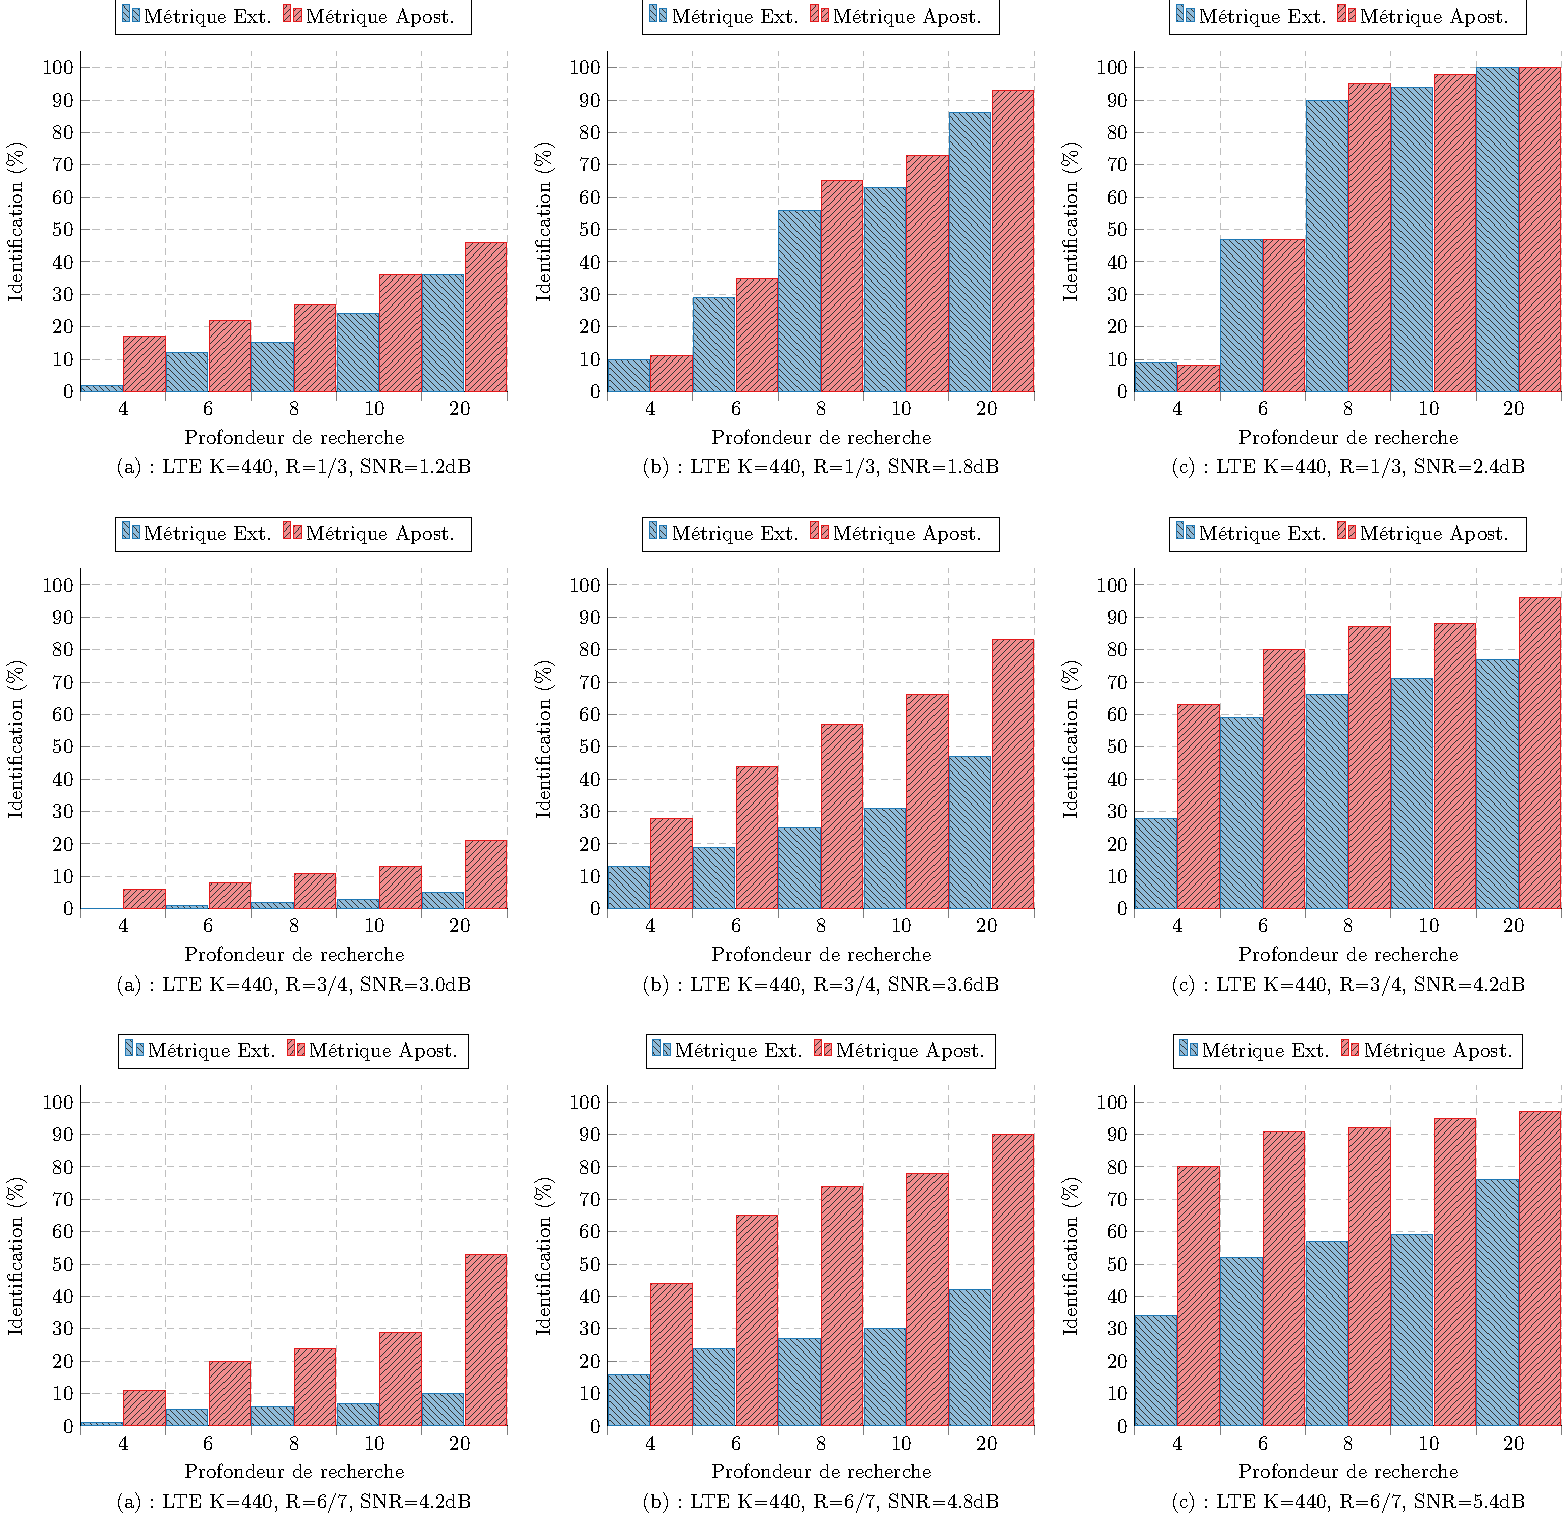
\includegraphics[width=1.05\textwidth]{main/ch3_fig/id2/dvb/tikz/440.pdf}
	\caption{Pourcentage d'identification pour différents turbo codes du standard DVB-RCS K=440, R=1/3, 3/4 et 6/7.
	Décodage EML-MAP itérant 8 fois. \label{fig:dvb752}}
\end{figure}}
{}
\end{document}
